% 第五章 整环中的不可约性与因子分解 --- 中译
% 原书 pp. 244--... (Aluffi, Algebra: Chapter 0, Chapter V).
% 本文件进度: §\ref{sec:chain-conditions} 已译 (2026-08-30); §\ref{sec:ufds-pids-euclidean} 以下待续.

\chapter{整环中的不可约性与因子分解}
\label{chap:integral-domains}


% ===== 记号索引 v1 集中埋点 (页码参考原书书页; 首次出现位置待人工校对) =====
% 本章记号条目（2 条）。OCR 已做最佳校正，但部分符号字形与首次
% 出现位置仍待逐条人工复核（页码沿用原书第 699 页 Index of Notation）。
% ===== /记号索引 =====
\index[sym1]{$R_{\mathfrak{p}}$@$R_{\mathfrak{p}}$}
\index[sym1]{$S^{-1}R$@$S^{-1}R$}
我们把注意力重新转回环上, 并分析几类有用的整环. 本章的一个主导主题是因子分解问题: 我们将处理环中元素的因子分解的存在性与唯一性, 把诸如 $\Z$ 或 $k[x]$ ($k$ 是域) 这类环的良好因子分解性质抽象为整环的整个族类. 读者不妨把下面这幅图景与本章的前半部分联系起来:

\begin{center}
\begin{tikzpicture}[scale=.68,line width=.5pt]
\filldraw[fill=gray!45] (0,0) ellipse (6 and 3.4);
\filldraw[fill=gray!25] (0,-.35) ellipse (5.5 and 2.9);
\draw (-.8,-.65) ellipse (4.4 and 2.5);
\draw (.8,-.65) ellipse (4.4 and 2.5);
\filldraw[fill=gray!15] (0,-1) ellipse (3 and 1.7);
\filldraw[fill=gray!8] (0,-1.35) ellipse (2.3 and 1.15);
\filldraw[fill=white] (0,-1.7) ellipse (1.1 and .6);
\node at (0,2.9) {整环};
\node at (0,2.1) {存在因子分解的整环};
\node[rotate=30] at (-3.3,.7) {UFD};
\node[rotate=-35] at (3,.7) {Noether 整环};
\node at (0,.3) {PID};
\node at (0,-.65) {Euclid 整环};
\node at (0,-1.7) {域};
\end{tikzpicture}
\end{center}
\index{huan@环(ring)!zhenghuan@整环(integral domain)}

统一假设: 本章考虑的所有环都是交换的\footnote{此外, 回想我们的所有环都有单位元 $1$; 参见定义~III.\ref{def:ring}.}. 事实上, 我们将考虑的大部分特殊环类都是整环, 也就是说, 有单位元且无非零零因子的交换环 (参见定义~III.\ref{def:integral-domain}).

\section{链条件与因子分解的存在性}
\label{sec:chain-conditions}

\subsection{Noether 环重访}
\label{subsec:noetherian-rings-revisited}

设 $R$ 是交换环. 回想 $R$ 称为 \emph{Noether 的}\index{noetherhuan@Noether 环(Noetherian ring)}, 如果 $R$ 的每个理想都是有限生成的 (定义~III.\ref{def:noetherian}). 事实上, 这是相应的模定义的一个特例: 环 $R$ 上的模 $M$ 称为 \emph{Noether 的}, 如果 $M$ 的每个子模都是有限生成的 (定义~III.\ref{def:noetherian-module}). 在 §III.\ref{subsec:noetherian-modules} 中我们已经验证, 这个条件沿正合列保持: 若 $M,N,P$ 是 $R$-模且
\[
\begin{tikzcd}
0 \ar[r] & N \ar[r] & M \ar[r] & P \ar[r] & 0
\end{tikzcd}
\]
是 $R$-模的正合列, 则 $M$ 是 Noether 的, 当且仅当 $N$ 与 $P$ 都是 Noether 的 (命题~III.\ref{prop:noetherian-extension}, 此处用 \S III.\ref{subsec:complexes} 中引入的语言重述\erratumfootnote{根据官方勘误, 此处注明引用命题是用短正合列语言重述 (restated here using the language introduced in \S III.\ref{subsec:complexes}).}). 这一事实的一个简单而有用的推论是: Noether 环上的每个有限生成模都是 Noether 的 (推论~III.\ref{cor:noetherian-fg}).

\index{Noether@Noether}Noether 条件还可以用其他方式表达, 熟悉它们是有益的.

\begin{proposition}\label{prop:noeth-acc}
设 $R$ 是交换环, $M$ 是 $R$-模. 则以下条件等价:
\begin{enumerate}[label=(\arabic*)]
\item $M$ 是 Noether 的; 也就是说, $M$ 的每个子模都是有限生成的.
\item $M$ 的子模的每条升链\index{shengliantiaojian@升链条件(ascending chain condition)}都稳定; 也就是说, 若
\[
N_1 \subseteq N_2 \subseteq N_3 \subseteq \cdots
\]
是 $M$ 的一串子模, 则存在 $i$ 使得 $N_i = N_{i+1} = N_{i+2} = \cdots$.
\item $M$ 的子模的每个非空族关于包含关系都有极大元.
\end{enumerate}
这里列出的第二个条件称为子模的\emph{升链条件} (a.c.c.). 取 $M = R$, 命题~\ref{prop:noeth-acc} 告诉我们 (除其他外): 一个环是 Noether 的, 当且仅当其理想满足升链条件.
\end{proposition}

\begin{proof}
(1)$\Rightarrow$(2): 设 $M$ 是 Noether 的, 并设
\[
N_1 \subseteq N_2 \subseteq N_3 \subseteq \cdots
\]
是 $M$ 的一串子模. 考虑并集 $N = \bigcup_i N_i$; 读者将验证 $N$ 是 $M$ 的子模. 由于 $M$ 是 Noether 的, $N$ 有限生成, 设 $N = (n_1,\dots,n_r)$. 现在 $n_k \in N \implies$ 对某个 $i_k$ 有 $n_k \in N_{i_k}$; 令 $i$ 为 $i_1,\dots,i_r$ 中的最大者\erratumfootnote{根据官方勘误, 将下标明确为 $i_k$, 并令 $i$ 为 $i_1,\dots,i_r$ 中的最大者 (letting $i$ be the largest among $i_1,\dots,i_r$).}, 可见存在 $i$ 使得所有 $n_1,\dots,n_r$ 都包含于 $N_i$. 但于是 $N \subseteq N_i$, 而由于 $N_i \subseteq N_{i+1} \subseteq \cdots$ 都包含于 $N = N_i$, 推出 $N_i = N_{i+1} = N_{i+2} = \cdots$, 如所求.

(2)$\Rightarrow$(3): 反设 $M$ 有一个不含极大元的子模族 $\mathcal{F}$. 如下构造一条不稳定的升链: 任取 $\mathcal{F}$ 中一个元素 $N_1$; 由于 $N_1$ 在 $\mathcal{F}$ 中不是极大的, 存在 $\mathcal{F}$ 中元素 $N_2$ 使得 $N_1 \subsetneq N_2$; 由于 $N_2$ 在 $\mathcal{F}$ 中不是极大的, 存在 $\mathcal{F}$ 中元素 $N_3$ 使得 $N_2 \subsetneq N_3$; 依此类推. 这条链
\[
N_1 \subsetneq N_2 \subsetneq N_3 \subsetneq \cdots
\]
不稳定, 表明 (2) 不成立.

(3)$\Rightarrow$(1): 设 (3) 成立, 并设 $N$ 是 $M$ 的子模. 令 $\mathcal{F}$ 为 $N$ 的有限生成子模组成的族. 这个族非空 (因为 $(0)\in\mathcal{F}$); 因此它有极大元 $N'$. 设 $N' = (n_1,\dots,n_r)$. 现在宣称 $N' = N$: 事实上, 设 $n\in N$; 子模 $(n_1,\dots,n_r,n)$ 是有限生成的, 因而属于 $\mathcal{F}$; 由于它包含 $N'$ 而 $N'$ 是极大的, 必有 $(n_1,\dots,n_r,n) = N'$; 特别地 $n\in N'$, 如所求.

这表明 $N = N'$ 是有限生成的, 而由于 $N\subseteq M$ 是任意的, 推出 $M$ 是 Noether 的.
\end{proof}

Noether 环是一类非常有用且灵活的环. 在 §III.\ref{subsec:finite-type} 中我们提到了一个重要的结论: Noether 环上的每个有限型代数都是 Noether 的. ``有限型 (交换) 代数'' 只是多项式环的商 (§III.\ref{subsec:finite-type}) 的一个花哨名称, 所以这个结论说的是:

\index{ji@基(basis)!chaoyue@超越(transcendence)}\index{ji@基(basis)!biaozhun@标准(standard)}\index{ji@基(basis)!youxu@有序(ordered)}\begin{theorem}\label{thm:hilbert-basis}
设 $R$ 是 Noether 环, $J$ 是多项式环 $R[x_1,\dots,x_n]$ 的一个理想. 则环 $R[x_1,\dots,x_n]/J$ 是 Noether 的\index{hilbertjidingli@Hilbert 基定理(Hilbert's basis theorem)}.
\end{theorem}

注意有限型 $R$-代数一般远非作为 $R$-模有限生成 (再参见 §III.\ref{subsec:finite-type}), 所以指望它们作为 $R$-模是 Noether 的未免愚蠢. 它们作为环 (即作为自身上的模) 竟是 Noether 的, 这给了我们一大类的 Noether 环的例子, 其中包括 (经典) 代数几何与数论中的环. 因此, 多亏了定理~\ref{thm:hilbert-basis}, 数学的整个分支都变得稍稍更易处理了.

这个深刻结论的证明出奇地容易. 由习题~\ref{ex:noeth-quotient}, 只需证明
\[
\index{Noether@Noether!mo@模(module)}R\text{ Noether}\ \Rightarrow\ R[x_1,\dots,x_n]\text{ Noether};
\]
\index{guina@归纳(induction)!deyuanli@的原理(principle of)}而一个简单的归纳把这一陈述归结为如下特例, 它有一个显赫的名字:

\begin{lemma}[Hilbert 基定理]\label{lem:hilbert-basis}
$R$ Noether $\Rightarrow$ $R[x]$ Noether.
\end{lemma}

\begin{proof}
设 $R$ 是 Noether 的, $I$ 是 $R[x]$ 的理想. 我们要证明 $I$ 有限生成.

回想若 $f(x) = a_d x^d + a_{d-1}x^{d-1} + \cdots + a_0 \in R[x]$ 且 $a_d\neq 0$, 则 $a_d$ 称为 $f(x)$ 的\emph{首项系数}\index{shouxianxishu@首项系数(leading coefficient)}. 考虑 $R$ 的如下子集:
\[
A = \{0\}\ \cup\ \{a\in R \mid a\text{ 是 } I\text{ 中某个元素的首项系数}\}.
\]
显然 $A$ 是 $R$ 的理想 (习题~\ref{ex:leading-ideal}); 由于 $R$ 是 Noether 的, $A$ 有限生成. 于是存在 $I$ 中的元素 $f_1(x),\dots,f_r(x)$, 其首项系数 $a_1,\dots,a_r$ 作为 $R$ 的理想生成 $A$.

现在令 $d_i$ 为 $f_i(x)$ 的次数, 并令 $d$ 为这些次数中的最大者. 考虑 $R$-子模
\[
M = (1,x,x^2,\dots,x^{d-1}) \subseteq R[x],
\]
即由次数 $< d$ 的多项式组成的 $R$-模. 由于 $M$ 作为 $R$-模有限生成, 它是 Noether $R$-模 (由推论~III.\ref{cor:noetherian-fg}). 因此, 其子模 $M\cap I$ 作为 $R$ 有限生成, 设为由 $I$ 中的元素 $g_1(x),\dots,g_s(x)$ 生成.

\begin{claim}\label{claim:hilbert-basis}
$I = (f_1(x),\dots,f_r(x),g_1(x),\dots,g_s(x))$.
\end{claim}
这个断言就推出了引理的陈述. 为证此断言, 我们只需证明反向包含; 为此, 任取 $\alpha(x)\in I$ 为 $I$ 中任意多项式. 若 $\deg\alpha(x)\geq d$, 令 $a$ 为 $\alpha(x)$ 的首项系数. 则 $a\in A$, 故存在 $b_1,\dots,b_r\in R$ 使得
\[
a = b_1 a_1 + \cdots + b_r a_r.
\]
令 $e = \deg\alpha(x)$, 于是对所有 $i$ 有 $e\geq d_i$, 这说明
\[
\alpha(x) - b_1 x^{e-d_1}f_1(x) - \cdots - b_r x^{e-d_r}f_r(x)
\]
的次数 $< e$. 迭代这一手续, 我们得到 $R[x]$ 中一列多项式 $\beta_1(x),\dots,\beta_r(x)$ 使得
\[
\alpha(x) - \beta_1(x)f_1(x) - \cdots - \beta_r(x)f_r(x)
\]
的次数 $< d$. (若一开始就有 $\deg\alpha(x)<d$, 我们可取 $\beta_1(x)=\cdots=\beta_r(x)=0$, 得到同样的结果.)\erratumfootnote{根据官方勘误, 补充 $\deg\alpha(x)<d$ 时的平凡情形选取.} 但这把该元素放入 $M\cap I$; 因此存在 $c_1,\dots,c_s\in R$ 使得
\[
\alpha(x) - \beta_1(x)f_1(x) - \cdots - \beta_r(x)f_r(x) = c_1 g_1(x) + \cdots + c_s g_s(x),
\]
我们就完成了, 因为这验证了
\[
\alpha(x) = \beta_1(x)f_1(x) + \cdots + \beta_r(x)f_r(x) + c_1 g_1(x) + \cdots + c_s g_s(x) \in (f_1(x),\dots,f_r(x),g_1(x),\dots,g_s(x)),
\]
完成了断言~\ref{claim:hilbert-basis} 的证明, 从而完成了引理~\ref{lem:hilbert-basis} 的证明, 也就完成了定理~\ref{thm:hilbert-basis} 的证明.
\end{proof}

\subsection{素元与不可约元}
\label{subsec:prime-irreducible}

设 $R$ 是 (交换) 环, $a,b\in R$. 我们说 $a$ \emph{整除}\index{zhnegchu@整除(divides)} $b$, 或称 $a$ 是 $b$ 的\emph{因子}, 或称 $b$ 是 $a$ 的\emph{倍数}, 如果 $b\in (a)$, 即
\[
(\exists c\in R)\quad b = ac.
\]
我们用记号 $a\mid b$.

两个元素 $a,b$ \emph{相伴}\index{xiangban@相伴(associated)}, 如果 $(a) = (b)$, 即如果 $a\mid b$ 且 $b\mid a$.

\begin{lemma}\label{lem:associates}
设 $a,b$ 是整环 $R$ 的非零元素. 则 $a$ 与 $b$ 相伴, 当且仅当存在 $R$ 中的单位 $u$ 使得 $a = ub$.
\end{lemma}

\begin{proof}
设 $a,b$ 相伴. 则存在 $c,d\in R$ 使得
\[
b = ac,\qquad a = bd;
\]
因此 $a = bd = acd$, 即
\[
a(1 - cd) = 0.
\]
由于在整环中非零元素消去律成立\erratumfootnote{根据官方勘误, 原书英文此处修正动词单复数 holds.}, 这推出 $cd = 1$. 于是 $c$ 是单位, 如所求.

反向包含留给读者.
\end{proof}

顺带一提, 读者在此看到了为什么把注意力限制在整环上是方便的. 这个论证实际表明: 若在整环中 $(a)=(b)\neq(0)$ 且 $b=ca$, 则 $c$ 必为单位. 离开整环这个舒适的环境, 即便这种看来无害的陈述也可能失效: 在 $\Z/6\Z$ 中, $2$ 与 $4$ 的类按照我们的定义是相伴的, 且 $[4]_6=[2]_6\cdot[2]_6$, 但 $[2]_6$ 不是单位. 然而, $[4]_6=[5]_6\cdot[2]_6$, 而 $[5]_6$ 是单位, 因而这不是引理~\ref{lem:associates} 的反例. 事实上, 该引理在有非``无害''零因子的环中可能失效 (的确存在这样的概念).

上面回顾的概念直接推广了 $\Z$ 中的相应概念. 我们打算在更一般的整环中探索 $\Z$ 中其他常见概念的类似物, 比如 ``素性'' 与 ``不可约性''.

\begin{definition}\label{def:prime-irreducible}
设 $R$ 是整环.
\begin{itemize}
\item 元素 $a\in R$ 是\emph{素元}\index{suyuan@素元(prime element)}, 如果 $(a)$ 是素理想; 也就是说, $a$ 不是单位, 且 (参见命题~III.\ref{prop:prime-maximal-alt})
\[
a\mid bc\ \Rightarrow\ (a\mid b\ \text{或}\ a\mid c).
\]
\item 元素 $a\in R$ 是\emph{不可约元}\index{bukeduoyuan@不可约元(irreducible element)}, 如果 $a$ 不是单位, 且
\[
a = bc\ \Rightarrow\ (b\text{ 是单位或 }c\text{ 是单位}).
\]
\end{itemize}
\end{definition}

零元总是可约的. 思考 ``不可约元'' 这个概念还有几种等价的办法: 一个非零非单位 $a$ 不可约, 当且仅当
\begin{itemize}
\item $a = bc$ 蕴含 $a$ 与 $b$ 或 $c$ 相伴;
\item $a = bc$ 蕴含 $(a) = (b)$ 或 $(a) = (c)$ (引理~\ref{lem:associates});
\item $(a)\subseteq (b)$ 蕴含 $(b) = (a)$ 或 $(b) = (1)$ (习题~\ref{ex:irred-maximal-principal});
\item $(a)$ 在真主理想中极大 (只是把上一点换个说法!).
\end{itemize}

重要的一点是, 素性与不可约性并不等价; 这有点反直觉, 因为它们在 $\Z$ 中等价, 这一点读者应当验证\footnote{这一事实将被一般理论完全解释清楚, 所以读者应当立刻把它证出来.} (习题~\ref{ex:prime-irred-Z}). 一般成立的是: 素性强于不可约.

\begin{lemma}\label{lem:prime-irreducible}
设 $R$ 是整环, $a\in R$ 是非零素元. 则 $a$ 不可约.
\end{lemma}

\begin{proof}
由于 $(a)$ 是素理想, $(a)\neq (1)$; 故 $a$ 不是单位. 若 $a = bc$, 则 $bc = a\in (a)$; 因此由于 $(a)$ 是素理想, $b\in (a)$ 或 $c\in (a)$. 不妨设 $b\in (a)$, 则有 $(b)\subseteq (a)$. 另一方面 $a = bc$ 蕴含 $(a)\subseteq (b)$: 于是 $(a) = (b)$, 即 $a$ 与 $b$ 相伴, 如所求.
\end{proof}

我们不久将看到逆命题在何种情形下成立.

\subsection{分解为不可约元; 存在因子分解的整环}
\label{subsec:factorization-irreducibles}

\begin{definition}\label{def:factorization}
设 $R$ 是整环. 元素 $r\in R$ 有\emph{不可约元的因子分解} (或\emph{分解}), 如果存在不可约元 $q_1,\dots,q_n$ 使得 $r = q_1\cdots q_n$.
\end{definition}

这个因子分解是\emph{唯一的}, 如果诸 $q_i$ 由 $r$ 确定到只差次序与相伴, 也就是说, 如果每当
\[
r = q'_1\cdots q'_m
\]
是 $r$ 的另一种不可约元分解, 则 $m = n$, 且在 (可能) 重排因子后 $q'_i$ 与 $q_i$ 相伴.

\begin{definition}\label{def:domain-factorizations}
整环 $R$ 称为\emph{存在因子分解的整环}\index{cunzai-yinzibunjie@存在因子分解的整环(domain with factorizations)} (或说 ``$R$ 中存在因子分解''), 如果 $R$ 的每个非零、非单位元素 $r\in R$ 都有不可约元的因子分解.
\end{definition}

\begin{definition}\label{def:ufd}
整环 $R$ 是\emph{析因的}, 或称\emph{唯一分解整环}\index{weiyi-fenjie@唯一分解整环(UFD)} (unique factorization domain, 简称 UFD), 如果 $R$ 的每个非零、非单位元素 $r\in R$ 都有唯一的不可约元因子分解.
\end{definition}

定义~\ref{def:domain-factorizations} 引入的术语似乎不太标准; 相比之下, UFD 是著名的.

我们将在 §\ref{sec:ufds-pids-euclidean} 研究唯一分解条件. 眼下, 似乎值得花点时间思考因子分解的单纯存在性. 有趣的是, 这个条件被一类特殊理想的升链条件所蕴含.

\begin{proposition}\label{prop:acc-factorization}
设 $R$ 是整环, $r$ 是 $R$ 的一个非零、非单位元素. 假设主理想的每条升链
\[
(r)\subseteq (r_1)\subseteq (r_2)\subseteq (r_3)\subseteq \cdots
\]
都稳定. 则 $r$ 有不可约元的因子分解.
\end{proposition}

\begin{proof}
设 $r$ 没有不可约元的因子分解. 特别地, $r$ 自身不是不可约的; 于是存在 $r_1,s_1\in R$ 使得 $r = r_1 s_1$ 且 $(r)\subsetneq (r_1)$, $(r)\subsetneq (s_1)$. 如果 $r_1,s_1$ 都有不可约元的因子分解, 则这些分解的乘积给出 $r$ 的一个分解; 因此不妨设 (例如) $r_1$ 没有不可约元的因子分解. 于是我们有
\[
(r)\subsetneq (r_1)
\]
且 $r_1$ 没有因子分解; 迭代这一论证构造出一条无限递增的链
\[
(r)\subsetneq (r_1)\subsetneq (r_2)\subsetneq \cdots,
\]
与我们的假设矛盾.
\end{proof}

\index{lixiang@理想(ideal)!gen@根(radical)}于是, 在那些主理想满足升链条件的整环中, 因子分解存在. 这有下述直接而方便的推论:

\begin{corollary}\label{cor:noetherian-domain-factorization}
设 $R$ 是 Noether 整环\index{noetherzhengghuan@Noether 整环(Noetherian domain)}. 则在 $R$ 中因子分解存在.
\end{corollary}

\begin{proof}
由命题~\ref{prop:noeth-acc}, Noether 整环满足所有理想的升链条件.
\end{proof}

推论~\ref{cor:noetherian-domain-factorization} 验证了本章开头所呈现的图景的一部分: Noether 整环类包含于存在因子分解的整环类. 这个包含是真包含: 例如, 标准的非 Noether 环的例子
\[
\Z[x_1,x_2,x_3,\dots]
\]
(例~III.\ref{ex:infinitely-many-variables}) 的确有因子分解. 事实上, 每个给定的多项式 $f\in \Z[x_1,x_2,\dots]$ 只涉及有限多个变量\footnote{回想多项式是单项式的有限线性组合; 参见 §III.\ref{subsec:polynomial-rings}.}, 因此属于一个同构于普通多项式环 $\Z[x_1,\dots,x_n]$ 的子环; 进而, 这个子环包含 $f$ 的每个因子. 由此可见 (参见习题~\ref{ex:zinfinite-acc}), $\Z[x_1,x_2,\dots]$ 中主理想的升链条件成立, 因为它在 $\Z[x_1,\dots,x_n]$ 中成立 (因为这个环是 Noether 的, 由 Hilbert 基定理).

\subsection*{习题}
\phantomsection
\addcontentsline{toc}{subsection}{习题}

\begin{prob}
\label{ex:noeth-quotient}
$\triangleright$ 设 $R$ 是 Noether 环, $I$ 是 $R$ 的理想. 证明 $R/I$ 是 Noether 环. [§\ref{subsec:noetherian-rings-revisited}]
\end{prob}

\begin{prob}
\label{ex:hilbert-converse}
证明若 $R[x]$ 是 Noether 的, 则 $R$ 也是. (这是 Hilbert 基定理的``逆''.)
\end{prob}

\begin{prob}
\label{ex:kt-algebra}
设 $k$ 是域, $f\in k[x]$, $f\notin k$. 对每个包含 $k$ 与 $f$ 的 $k[x]$ 的子环 $R$, 通过把 $k$ 上的恒等映射延拓并把 $t$ 映到 $f$ 来定义同态 $\varphi : k[t]\to R$. 这使得每个这样的 $R$ 成为 $k[t]$-代数 (例~III.\ref{ex:R-algebra}).
\begin{itemize}
\item 证明 $k[x]$ 作为 $k[t]$-模是有限生成的.
\item 证明上述每个子环 $R$ 作为 $k[t]$-模是有限生成的.
\item 证明 $k[x]$ 的每个包含 $k$ 的子环都是 Noether 环.
\end{itemize}
\end{prob}

\begin{prob}
\label{ex:cont-functions-noeth}
设 $R$ 是区间 $[0,1]$ 上实值连续函数的环. 证明 $R$ 不是 Noether 的.
\end{prob}

\begin{prob}
\label{ex:powerset-noeth}
对哪些集合 $S$, 幂集环 $\mathcal{P}(S)$ 是 Noether 的? (参见习题~III.\ref{ex:powerset-ideals}.)
\end{prob}

\begin{prob}
\label{ex:leading-ideal}
$\triangleright$ 设 $I$ 是 $R[x]$ 的理想, $A\subseteq R$ 是定理~\ref{thm:hilbert-basis} 证明中所定义的集合. 证明 $A$ 是 $R$ 的理想. [§\ref{subsec:noetherian-rings-revisited}]
\end{prob}

\begin{prob}
\label{ex:power-series-noeth}
证明若 $R$ 是 Noether 环, 则幂级数环\index{mishubianhuan@幂级数环(ring of power series)} $R[[x]]$ (参见 §III.\ref{subsec:polynomial-rings}) 也是 Noether 的. (提示: 幂级数 $\sum_{i=0}^\infty a_i x^i$ 的\emph{阶}是使 $a_i\neq 0$ 的最小 $i$; 其首项系数就是 $a_i$. 设 $I$ 是 $R[[x]]$ 的理想, 令 $A_i\subseteq R$ 为 $I$ 中阶为 $i$ 的幂级数的首项系数连同 $0$ 组成的集合\erratumfootnote{根据官方勘误, 明确补上“设 $I$ 是 $R[[x]]$ 的理想”的前提.}. 证明 $A_i$ 是 $R$ 的理想且 $A_0\subseteq A_1\subseteq A_2\subseteq \cdots$. 由于 $R$ 是 Noether 的, 这个序列稳定, 且每个 $A_i$ 同理有限生成. 现在套用引理~\ref{lem:hilbert-basis} 的证明.)
\end{prob}

\begin{prob}
\label{ex:noeth-ideal-prime-product}
证明 Noether 环 $R$ 的每个理想都包含一个素理想的乘积. (提示: 令 $\mathcal{F}$ 为不含素理想之有限乘积的理想组成的族. 若 $\mathcal{F}$ 非空, 由于 $R$ 是 Noether 的, 它有极大元 $M$. 由于 $M\in\mathcal{F}$, $M$ 自身不是素的, 故存在 $a,b\in R$ 使得 $a\notin M$, $b\notin M$, 但 $ab\in M$. 这有什么问题?)
\end{prob}

\begin{prob}
\label{ex:min-primes-finite}
$\neg$ 设 $R$ 是交换环, $I\subseteq R$ 是真理想. 读者将在习题~\ref{ex:minimal-primes} 中证明: 包含 $I$ 的素理想组成的集合有极小元 (即 $I$ 的\emph{极小素}). 证明若 $R$ 是 Noether 的, 则 $I$ 的极小素的集合有限. (提示: 令 $\mathcal{F}$ 为具有无穷多个极小素的理想组成的族. 若 $\mathcal{F}\neq\varnothing$, 注意 $\mathcal{F}$ 必有极大元 $J$, 且 $J$ 自身不是素理想. 找出严格大于 $J$ 的理想 $J_1,J_2$ 使得 $J_1 J_2\subseteq J$, 并导出矛盾.)\erratumfootnote{根据官方勘误, 将极大元记号由 $I$ 改为 $J$ 以免与题目中的 $I$ 混淆, 并明确族 $\mathcal{F}$ 为具有无穷多个极小素的理想族.} [VI.\ref{ex:minimal-primes-ass}]
\end{prob}

\begin{prob}
\label{ex:artinian}
$\neg$ 由命题~\ref{prop:noeth-acc}, 环 $R$ 是 Noether 的, 当且仅当它满足理想的升链条件. 环称为\emph{阿廷的}\index{atinghuan@阿廷环(Artinian ring)} (Artinian), 如果它满足理想的降链条件\index{jiangliantiaojian@降链条件(descending chain condition)} (d.c.c.). 证明若 $R$ 是阿廷的且 $I\subseteq R$ 是理想, 则 $R/I$ 是阿廷的. 证明若 $R$ 是阿廷整环, 则它是域. (提示: 设 $r\in R$, $r\neq 0$. 理想 $(r^n)$ 形成降链; 故对某个 $n$ 有 $(r^n) = (r^{n+1})$. 于是……) 证明阿廷环的 Krull 维数\index{krullweishu@Krull 维数(Krull dimension)}为 $0$ (也就是说, 阿廷环中的素理想都是极大的\footnote{可以证明阿廷环必是 Noether 的; 事实上, 一个环是阿廷的, 当且仅当它是 Noether 的且 Krull 维数为 $0$. 因此, d.c.c. 蕴含 a.c.c., 而 a.c.c. 蕴含 d.c.c. 当且仅当所有素理想都是极大的.}). [\ref{ex:pid-artinian-quotient}]
\end{prob}

\begin{prob}
\label{ex:associate-equiv}
证明 ``相伴'' 关系是一个等价关系.
\end{prob}

\begin{prob}
\label{ex:irred-maximal-principal}
$\triangleright$ 设 $R$ 是整环. 对非零元素 $a\in R$, 证明 $a$ 不可约, 当且仅当 $(a)$ 在 $R$ 的真主理想中极大. [§\ref{subsec:prime-irreducible}, §\ref{subsec:pid-ufd}]
\end{prob}

\begin{prob}
\label{ex:prime-irred-Z}
$\triangleright$ 证明在 $\Z$ 中对非零元素有素元 $\Leftrightarrow$ 不可约元. [§\ref{subsec:prime-irreducible}, §\ref{subsec:pid-ufd}]
\end{prob}

\begin{prob}
\label{ex:class-prime}
对交换环 $R$ 中的元素 $a,b$, 证明 $a$ 在 $R/(b)$ 中的类素, 当且仅当 $b$ 在 $R/(a)$ 中的类素.
\end{prob}

\begin{prob}
\label{ex:zinfinite-acc}
$\triangleright$ 把 $S = \Z[x_1,\dots,x_n]$ 以自然方式等同于可数无穷多变量多项式环 $R = \Z[x_1,x_2,x_3,\dots]$ 的子环. 证明若 $f\in S$ 且在 $R$ 中 $(f)\subseteq (g)$, 则 $g\in S$. 推出 $R$ 中主理想的升链条件成立, 从而 $R$ 是存在因子分解的整环. [§\ref{subsec:factorization-irreducibles}, §\ref{subsec:ufd-poly}]
\end{prob}

\begin{prob}
\label{ex:acc-infinite}
设 $R=\Z[x_1,x_2,x_3,\ldots]/(x_1-x_2^2,x_2-x_3^2,\ldots)$. $R$ 中主理想的升链条件成立吗?
\end{prob}

\begin{prob}
\label{ex:zsqrt5}
$\triangleright$ 考虑 $\CC$ 的子环
\[
\Z[\sqrt{-5}] := \{a + b\sqrt{-5} \mid a,b\in\Z\}.
\]
\begin{itemize}
\item 证明这个环同构于 $\Z[t]/(t^2 + 5)$.
\item 证明它是 Noether 整环.
\item 在 $\Z[\sqrt{-5}]$ 上定义 ``范数'' $N$ 如下: 令 $N(a + b\sqrt{-5}) = a^2 + 5b^2$. 证明 $N(zw) = N(z)N(w)$. (参见习题~III.\ref{ex:Q-sqrt-d}.)
\item 证明 $\Z[\sqrt{-5}]$ 中的单位是 $\pm 1$. (用前一点.)
\item 证明 $2, 3, 1 + \sqrt{-5}, 1 - \sqrt{-5}$ 都是 $\Z[\sqrt{-5}]$ 的不可约而非相伴的元素.
\item 证明上面列出的元素中没有一个是素元. (证明由这些元素生成的理想作商所得的环不是整环.)
\item 证明 $\Z[\sqrt{-5}]$ 不是 UFD.
\end{itemize}
[§\ref{subsec:ufd-characterization}, \ref{ex:zd19-not-euclidean}, \ref{ex:zsqrt-2-euclidean}]
\end{prob}
\section{UFD、PID 与 Euclid 整环}
\label{sec:ufds-pids-euclidean}

\subsection{不可约因子与最大公因子}
\label{subsec:irreducible-gcd}

整环 $R$ 是 UFD, 如果 $R$ 中因子分解存在, 并且如定义~\ref{def:factorization} 的意义下唯一.
因此, 在 UFD 中, 所有元素 (除 $0$ 与单位之外) 都决定一个不可约因子的多重集
(``带重数的元素集合''; 参见 §I.\ref{subsec:sets}), 这个多重集由相伴关系确定到相伴.
\index{duozhongji@多重集(multiset)!duichenxing@对称性(symmetry)}我们也可以约定单位没有因子; 也就是说, 相应的多重集是空的.

\noindent 下面的平凡注记是大多数关于 UFD 的初等事实的根源, 例如定理~\ref{thm:ufd-char} 的刻画:

\begin{lemma}\label{lem:ufd-multiset}
设 $R$ 是 UFD, $a,b,c$ 是 $R$ 的非零元素. 则
\begin{itemize}
\item[(a)] $a\mid b$ $\iff$ $a$ 的不可约因子多重集包含于 $b$ 的不可约因子多重集;
\item[(b)] $a$ 与 $b$ 相伴 (即 $(a)=(b)$) $\iff$ 这两个多重集重合;
\item[(c)] $ab$ 的不可约因子就是 $a$ 与 $b$ 的所有不可约因子的并.
\end{itemize}
\end{lemma}

\noindent 证明留给读者 (习题~\ref{ex:ufd-lemmas}). 在 UFD 中工作的好处在于: 关于环中元素的环论命题,
\index{duozhongji@多重集(multiset)!Tarski@Tarski!Alfred@Alfred}往往可以借助引理~\ref{lem:ufd-multiset} 归结为关于不可约元素多重集的直白集合论命题.

\noindent 这一机制的一个重要例子是最大公因子的存在性. 在前面的章节中我们已经大量使用了这个概念
(至少对整数而言); 现在我们可以从更技术的角度来理解它.

\begin{definition}\label{def:gcd}
设 $R$ 是整环, $a,b\in R$. 元素 $d\in R$ 称为 $a$ 与 $b$ 的一个\emph{最大公因子}\index{zuida-gongyinshi@最大公因子(greatest common divisor)} (常缩写为
``gcd''), 如果 $(a,b)\subseteq (d)$, 并且 $(d)$ 是 $R$ 中具有此性质的最小的主理想.
\end{definition}

\noindent 换言之, $d$ 是 $a$ 与 $b$ 的最大公因子, 如果 $d\mid a$, $d\mid b$, 并且
\[
c\mid a,\ c\mid b \quad\Longrightarrow\quad c\mid d.
\]
这个定义立即可以推广到任意有限多个元素. 注意, 这一规定并没有唯一地确定最大公因子:
若 $d$ 是 $a$ 与 $b$ 的最大公因子, 则 $d$ 的每个相伴元也都是. 因此, 记号 ``$\gcd(a,b)$''
只应用来表示由 $a,b$ 的所有最大公因子组成的相伴类. 当然, 在这一点上语言常常 (无害地) 被滥用.
例如, 我们能谈论两个整数的最大公因子, 是因为在 $\Z$ 中有一种方便的方式在每个相伴整数类中挑出一个特殊的元素
(即非负的那个).

\noindent 还要注意的是, 最大公因子未必存在 (参见习题~\ref{ex:subring-nodeg1}); 但在 UFD 中确实存在:

\begin{lemma}\label{lem:ufd-gcd}
设 $R$ 是 UFD, $a,b$ 是 $R$ 的非零元素. 则 $a,b$ 有最大公因子.
\end{lemma}

\begin{proof}
我们可以写出
\[
a = u\,q_1^{\alpha_1}\cdots q_r^{\alpha_r},\qquad
b = v\,q_1^{\beta_1}\cdots q_r^{\beta_r},
\]
其中 $u,v$ 是单位, $q_i$ 是不可约元, 当 $i\neq j$ 时 $q_i$ 不与 $q_j$ 相伴, 且 $\alpha_i\ge 0$, $\beta_i\ge 0$
(于是 $a$ 的不可约因子多重集由那些使 $\alpha_i>0$ 的 $q_i$ 组成, 类似地 $b$ 的由使 $\beta_i>0$ 的 $q_i$ 组成;
单位 $u,v$ 被包括进来, 是因为不可约因子只定义到相伴关系). 我们断言
\[
d = q_1^{\min(\alpha_1,\beta_1)}\cdots q_r^{\min(\alpha_r,\beta_r)}
\]
是 $a$ 与 $b$ 的一个最大公因子. 的确, $d$ 显然是 $a$ 与 $b$ 的因子; 而如果 $c$ 也整除 $a$ 与 $b$, 那么由引理~\ref{lem:ufd-multiset},
$c$ 的因子多重集必须同时包含于 $a$ 与 $b$ 的因子多重集中; 也就是说,
\[
c = w\,q_1^{\gamma_1}\cdots q_r^{\gamma_r},
\]
其中 $w$ 是单位, 且 $\gamma_i\le \alpha_i$, $\gamma_i\le \beta_i$. 这推出 $\gamma_i\le \min(\alpha_i,\beta_i)$,
从而 $c\mid d$ (再次由引理~\ref{lem:ufd-multiset}), 如所求.
\end{proof}

\noindent 当然, 上述证明中所用的论证推广了在 $\Z$ 中计算最大公因子的一条标准途径: 在素因子分解中取最小的指数.
但要注意, 这并不是在 $\Z$ 中计算最大公因子的唯一方法; 我们马上还会回到这一点. 事实上, $\Z$ 中最大公因子具有某些不应在更一般的整环中期待的性质;

\subsection{UFD 的刻画}
\label{subsec:ufd-characterization}

\noindent 例如, 习题~II.\ref{ex:bezout} 的结果并不能推广到任意整环 (甚至不能推广到任意 UFD), 这一点读者将在习题~\ref{ex:xy-gcd} 中验证.

\index{huan@环(ring)!de Krull weishu@的 Krull 维数(Krull dimension of a)!jubu@局部(local)}构造唯一因子分解不成立的整环是容易的. 勤勉的读者已经分析过一个例子 (习题~\ref{ex:zsqrt5}); 再看一个,
\index{huan@环(ring)!jubuhua@局部化(localization)}在整环
\[
R = \CC[x,y,z,w]/(xw-yz)
\]\footnote{在代数几何中, 这是 $\mathbb A^4$ 中一个二次锥的环. 这个锥的顶点 (原点) 是奇点, 这与 $R$ 不是 UFD 有关.}
中, (这些元素的类) $x,y,z,w$ 都是不可约的, 且彼此不相伴; 由于在 $R$ 中 $xw-yz=0$, 元素 $xw$ 有两个相异的不可约分解:
$x\cdot w=y\cdot z$.

\noindent 注意, 由定理~\ref{thm:hilbert-basis}, 这个环是 Noether 的 (特别地, $R$ 中因子分解确实存在). 因此, 存在不是 UFD 的 Noether 整环.

\noindent 还要注意, 这个环提供了一个反例, 说明引理~\ref{lem:prime-irreducible} 的``逆命题''不成立: 的确, (类) $x$ 是不可约的, 但商
\[
R/(x) \cong \CC[x,y,z,w]/(xw-yz,x)\cong \CC[y,z,w]/(yz)
\]
不是整环 (因为 $y\neq 0$, $z\neq 0$, 但在该环中 $yz=0$); 也就是说, $x$ 不是素元.

\noindent 事实上, 也许有点出人意料, 唯一因子分解的问题与素性和不可约性之间的关系纠缠不清. 的确, 引理~\ref{lem:prime-irreducible} 的``逆命题''在 UFD 中成立:

\begin{lemma}\label{lem:irred-prime-ufd}
设 $R$ 是 UFD, $a$ 是 $R$ 的不可约元. 则 $a$ 是素元.
\end{lemma}

\begin{proof}
按不可约元的定义, $a$ 不是单位. 设 $bc\in (a)$; 于是 $(bc)\subseteq (a)$, 由引理~\ref{lem:ufd-multiset}, $a$ 的不可约因子
(即 $a$ 本身) 必属于 $b$ 或 $c$ 的因子之中. 第一种情形有 $b\in (a)$, 第二种情形有 $c\in (a)$.
这就表明 $(a)$ 是素理想, 如所求.
\end{proof}

\noindent 事实上, 还不止于此. 只要主理想的升链条件成立, 那么 UFD 就由不可约性与素性的等价来刻画.

\begin{theorem}\label{thm:ufd-char}
整环 $R$ 是 UFD, 当且仅当
\begin{itemize}
\item $R$ 中主理想的升链条件 (a.c.c.) 成立, 且
\item $R$ 的每个不可约元都是素元.
\end{itemize}
\end{theorem}

\begin{proof}
($\Rightarrow$) 设 $R$ 是 UFD. 引理~\ref{lem:irred-prime-ufd} 表明 $R$ 的不可约元都是素元. 为证 $R$ 中主理想的升链条件成立,
考虑一条升链
\[
(r_1)\subseteq (r_2)\subseteq (r_3)\subseteq \cdots
\]
\index{duozhongji@多重集(multiset)!zhangliang@张量(tensor)}由引理~\ref{lem:ufd-multiset}, 这条链决定一条相应的不可约因子多重集的降链. 有限多重集的降链显然稳定, 从而 (再由引理~\ref{lem:ufd-multiset})
对充分大的 $i$ 有 $(r_i)=(r_{i+1})=(r_{i+2})=\cdots$.

($\Leftarrow$) 现在设 $R$ 满足主理想的升链条件, 且不可约元都是素元. 命题~\ref{prop:acc-factorization} 推出 $R$ 中因子分解存在;
我们只需验证唯一性. 设 $q_1,\dots,q_m$ 与 $q'_1,\dots,q'_n$ 是 $R$ 的不可约元, 并设
\[
q_1\cdots q_m = q'_1\cdots q'_n.
\]
则 $q'_1\cdots q'_n\in (q_1)$, 而 $(q_1)$ 是素理想 (由假设); 于是某个 $q'_i\in (q_1)$,
在调整因子次序后可设 $i=1$. 因此 $q'_1 = u q_1$ 对某个 $u\in R$ 成立. 由于 $q'_1$ 不可约且 $q_1$ 不是单位,
必然 $u$ 是单位. 于是 $q_1$ 与 $q'_1$ 相伴. 消去 $q_1$ 并将 $q'_2$ 替换为 $u q'_2$, 我们得到
\[
q_2\cdots q_m = q'_2\cdots q'_n.
\]
重复这个过程, 将各因子逐一配对. 显然 $m=n$, 否则我们将得到 $1=$ 一些不可约元的乘积, 这与不可约元不是单位矛盾.
\end{proof}

\noindent 定理~\ref{thm:ufd-char} 是一个漂亮的命题, 但它并没有让检验一个给定的环是否真的是 UFD 变得特别容易. 这种情况与 Noether 环颇有相似之处:
\index{huan@环(ring)!Noether@Noether}升链条件是 Noether 条件的精确等价表述, 但在实践中人们更常依赖别的工具 (例如 Hilbert 基定理) 来断定一个给定的环是 Noether 的.
Hilbert 基定理对唯一分解整环是否有类似的类比? 回答这个问题需要一些准备工作, 我们将在 §\ref{sec:ufd-poly-rings} 回到它.

\subsection{PID \texorpdfstring{$\Rightarrow$}{=>} UFD}
\label{subsec:pid-ufd}

有简单的办法造出 UFD 的例子. 回想 (由 §III.\ref{subsec:prime-maximal}) \emph{主理想整环}\index{zhulixiang-zhenghuan@主理想整环(principal ideal domain)} (缩写为 PID) 是指每个理想都是主理想的整环. 在 §III.\ref{subsec:prime-maximal} 中我们已观察到
\begin{itemize}
\item PID 是 Noether 的.
\item $\Z$ 与 $k[x]$ (其中 $k$ 是域) 是 PID.
\item 若 $R$ 是 PID 且 $a,b\in R$, 则 $d$ 是 $a$ 与 $b$ 的最大公因子, 当且仅当 $(a,b)=(d)$. 特别地, 若 $d$ 是 PID $R$ 中 $a$ 与 $b$ 的最大公因子, 则 $d$ 是 $a$ 与 $b$ 的线性组合: 存在 $r,s\in R$ 使得 $d=ra+sb$.
\item 若 $I$ 是 PID 中的非零理想, 则 $I$ 是素理想, 当且仅当它是极大理想.
\end{itemize}
我们现在给这个清单加上重要的一条:

\begin{proposition}\label{prop:pid-ufd}
若 $R$ 是 PID, 则它是 UFD.
\end{proposition}

\begin{proof}
设 $R$ 是 PID. 由于 PID 是 Noether 的, 升链条件在 $R$ 中成立 (对所有理想, 因而特别地对所有主理想);
我们验证 $R$ 中不可约元都是素元, 于是由定理~\ref{thm:ufd-char} 推出 $R$ 是 UFD.

设 $a\in R$ 是不可约元, 并设 $bc\in (a)$; 我们要证明 $b$ 或 $c$ 属于 $(a)$. 若 $b\in (a)$, 则已证; 因此设 $b\notin (a)$.
于是 $(a,b)\supsetneq (a)$; 由于 $R$ 是 PID, 存在 $d\in R$ 使得 $(d)=(a,b)$, 从而 $(d)\supseteq (a)$. 这推出
$(a,b)=(d)=(1)$, 因为 $a$ 不可约, 而由不可约元生成的理想在主理想中极大 (参见习题~\ref{ex:irred-maximal-principal}). 于是存在 $r,s\in R$ 使得
$ra+sb=1$. 两边乘以 $c$, 我们得到
\[
c = rac + sbc \in (a),
\]
如所求.
\end{proof}

\noindent 特别地, 若 $k$ 是域, 则 $k[x]$ 是 UFD; 而 $\Z$ 是 UFD —— 但愿这不会让我们的读者大吃一惊%
\footnote{这个事实被称为\emph{算术基本定理}.}. 注意, 至此我们已经以完整的面貌重新得到了习题~\ref{ex:prime-irred-Z} 中所陈述的事实.

\noindent 命题~\ref{prop:pid-ufd} 也证实了本章开头那幅图的一个特征: PID 类包含在 UFD 类之中. 我们马上会看到这个包含是真包含, 也就是说, 存在不是 PID 的 UFD; 例如, $\Z[x]$ 不是 PID (习题~\ref{ex:rx-pid-field}), 然而
\[
\Z[x]\ \text{是唯一分解整环}
\]
这一点我们不久就能证明 (定理~\ref{thm:ufd-poly}). 事实上, 也存在不是 Noether 的 UFD, 正如图中所示; 不过, 这些例子最好在积累更多素材之后再讨论 (例~\ref{ex:nonnoeth-ufd}).

\noindent 读者已经可以通过思考下面这个 (上面回忆过且本质上同义反复) 的事实, 来感受 UFD 与 PID 之间的差距: 在 PID 中, $a,b$ 的最大公因子是 $a$ 与 $b$ 的线性组合. 这是一个很强的条件: 例如, 它刻画了 Noether 整环中的 PID (读者将验证, 习题~\ref{ex:noeth-linearcomb-pid}); 它在一般 UFD 中并不成立 (习题~\ref{ex:xy-gcd}).

\subsection{Euclid 整环 \texorpdfstring{$\Rightarrow$}{=>} PID}
\label{subsec:euclidean-pid}

$\Z$ 与 $k[x]$ (其中 $k$ 是域) 的优良性质使这两个环比 PID 还要特殊: 它们是\emph{Euclid 整环}\index{euclid-zhenghuan@Euclid 整环(Euclidean domain)}.

\noindent 非正式地说, Euclid 整环是可以做``带余除法''的环: 对 $\Z$ 与 $k[x]$ 都是如此, 如 §III.\ref{subsec:prime-maximal} 中所观察到的. 要点在于, 在 $\Z$ 与 $k[x]$ 中都可以定义元素``大小''的概念: 整数 $n$ 的 $\lvert n\rvert$, 以及多项式 $f(x)$ 的 $\deg f(x)$. 在两种情形中, 人们都能控制除法中``余式''的大小. Euclid 整环的定义正是抽象出了这一机制.

\noindent 为此, 整环 $R$ 上的一个\emph{赋值}\index{fuzhi@赋值(valuation)} 是任一函数 $v:R\setminus\{0\}\to \mathbb{Z}_{\ge 0}$%
\footnote{关于赋值的文献浩如烟海, 研究的是比这里所需的更精细的概念.}.

\index{fuzhi@赋值(valuation)!Euclid@Euclid}\index{fuzhi@赋值(valuation)!lisan@离散(discrete)}\index{fuzhi@赋值(valuation)!Dedekind–Hasse@Dedekind–Hasse}\begin{definition}\label{def:euclidean-valuation}
整环 $R$ 上的\emph{Euclid 赋值}是指满足如下性质的赋值%
\footnote{要求对所有非零 $a,b\in R$ 有 $v(ab)\ge v(b)$ 也并不罕见; 但在接下来的讨论中并不需要这一点, 参见习题~\ref{ex:euclidean-valuation-monotone}.}: 对所有 $a\in R$ 与所有非零 $b\in R$, 存在 $q,r\in R$ 使得
\[
a = qb + r,
\]
并且 $r=0$ 或 $v(r)<v(b)$. 整环 $R$ 若承认一个 Euclid 赋值, 就称为\emph{Euclid 整环}.
\end{definition}

\noindent 我们说 $q$ 是除法的\emph{商}, $r$ 是\emph{余式}. $\Z$ 与 $k[x]$ (其中 $k$ 是域) 中的带余除法给出了例子, 所以 $\Z$ 与 $k[x]$ 都是 Euclid 整环.

\begin{proposition}\label{prop:euclidean-pid}
设 $R$ 是 Euclid 整环. 则 $R$ 是 PID.
\end{proposition}

\noindent 证明模仿了在 $\Z$ 中遇到的情形 (命题~III.\ref{prop:Z-PID}) 与在 $k[x]$ 中遇到的情形 (读者大概已在习题~III.\ref{ex:kx-pid} 中做过了).

\begin{proof}
设 $I$ 是 $R$ 的理想; 我们要证 $I$ 是主理想. 若 $I=\{0\}$, 则无待证; 因此设 $I\neq\{0\}$. 赋值把 $I$ 的非零元映到 $\mathbb{Z}_{\ge 0}$ 的一个子集; 设 $b\in I$ 是赋值最小的元素. 我们断言 $I=(b)$; 于是 $I$ 是主理想, 如所求. 由于显然 $(b)\subseteq I$, 我们只需验证 $I\subseteq (b)$.

\noindent 为此, 设 $a\in I$ 并作带余除法: 我们有
\[
a = qb + r
\]
对某个 $q,r\in R$, 其中 $r=0$ 或 $v(r)<v(b)$. 但
\[
r = a - qb \in I;
\]
由 $v(b)$ 在 $I$ 的非零元中最小, 我们不可能有 $v(r)<v(b)$. 因此 $r=0$, 表明 $a=qb\in (b)$, 如所求.
\end{proof}

\noindent 命题~\ref{prop:euclidean-pid} 又证实了本章开头那幅图的一个特征: Euclid 整环类包含在主理想整环类之中.

\noindent 如该图所提示, 这个包含是真包含. 具体给出一个不是 Euclid 整环的 PID 例子并不容易, 但 PID 与 Euclid 整环之间的差距其实可以刻画得非常精确: PID 可以刻画为满足比``带余除法''更弱条件的整环.

\noindent 更确切地说, 一个\emph{Dedekind--Hasse 赋值}是指满足如下条件的赋值 $v$: 对所有 $a$ 与所有非零 $b$, 要么 $(a,b)=(b)$ (即 $b\mid a$), 要么存在非零元 $r\in (a,b)$ 使得 $v(r)<v(b)$\erratumfootnote{根据官方勘误, 明确要求 $b$ 非零以及 $r$ 非零.}. 后一条件等价于要求存在 $q,s\in R$ 使得 $as=bq+r$ 且 $v(r)<v(b)$; 因此 Euclid 赋值 (对其我们其实可以取 $s=1$) 是一种 Dedekind--Hasse 赋值. 不难证明整环是 PID, 当且仅当它承认一个 Dedekind--Hasse 赋值 (习题~\ref{ex:dedekind-hasse-pid}). 例如, 这可以用来证明环 $\Z[(1+\sqrt{-19})/2]$ 是 PID: 在习题~\ref{ex:zd19-not-euclidean} 中用来证明这个环不是 Euclid 整环的那个范数, 原来是一个 Dedekind--Hasse 赋值%
\footnote{这归结为逐个情形的分析, 我们很高兴把它留给最有耐心的读者.}. 于是, 这个环给出了一个不是 Euclid 整环的 PID 的例子.

\noindent Euclid 整环的一个优良特性 (也是它得名的缘由) 是存在计算最大公因子的有效算法: \emph{Euclid 算法}\index{oushi-suanfa@Euclid 算法(Euclidean algorithm)}. 由于 Euclid 整环是 PID, 从而是 UFD, 我们知道它们确有最大公因子. 然而, 从引理~\ref{lem:ufd-gcd} 的证明蒸馏出的``算法''极不实用: 如果为了计算两个整数 $a,b$ 的最大公因子而必须先对它们作因子分解, 那么对于几百位的整数 (以当前的技术与因子分解算法) 这本质上是做不到的. Euclid 算法绕过了因子分解的必要性: 上千位整数的最大公因子可以在一瞬间算出来.

\noindent 算法所依据的引理是如下平凡的普遍事实:

\begin{lemma}\label{lem:gcd-remainder}
设 $R$ 中 $a=bq+r$. 则 $(a,b)=(b,r)$.
\end{lemma}

\begin{proof}
的确, $r=a-bq\in (a,b)$, 证得 $(b,r)\subseteq (a,b)$; 而 $a=bq+r\in (b,r)$, 证得 $(a,b)\subseteq (b,r)$.
\end{proof}

\noindent 特别地,
\[
(\forall c\in R)\quad (a,b)\subseteq (c)\ \Longleftrightarrow\ (b,r)\subseteq (c);
\]
也就是说, $a,b$ 的公因子集合与 $b,r$ 的公因子集合重合. 因此,

\begin{corollary}\label{cor:gcd-remainder}
设 $a=bq+r$. 则 $a,b$ 有最大公因子, 当且仅当 $b,r$ 有最大公因子; 在此情形下 $\gcd(a,b)=\gcd(b,r)$.
\end{corollary}

\noindent 当然, ``$\gcd(a,b)=\gcd(b,r)$'' 的意思是这两个相伴元类重合.

\noindent 这些考虑在任何整环上都成立; 现在设 $R$ 是 Euclid 整环. 则我们可以用带余除法来控制余式 $r$. 给定 $R$ 中两个元素 $a,b$, $b\neq 0$, 我们可以反复作带余除法:
\[
\begin{aligned}
a &= bq_1 + r_1,\\
b &= r_1q_2 + r_2,\\
r_1 &= r_2q_3 + r_3,
\end{aligned}
\]
只要余式 $r_i$ 非零.

\begin{claim}\label{claim:euclid-terminates}
这个过程终止: 即存在 $N$ 使得 $r_N=0$.
\end{claim}

\begin{proof}
表中每一行都是一次带余除法. 若没有 $r_i$ 为零, 我们就会得到一列严格递减的非负整数序列, 荒谬.
\end{proof}

\noindent 于是带余除法的表必如下形: 令 $r_0=b$, 且 $r_{N-1}\neq 0$.
\[
\begin{aligned}
a &= r_0q_1 + r_1,\\
b &= r_1q_2 + r_2,\\
r_1 &= r_2q_3 + r_3,\\
&\ \,\vdots\\
r_{N-3} &= r_{N-2}q_{N-1} + r_{N-1},\\
r_{N-2} &= r_{N-1}q_N.
\end{aligned}
\]

\begin{proposition}\label{prop:euclid-gcd}
沿用上述记号, $r_{N-1}$ 是 $a,b$ 的一个最大公因子.
\end{proposition}

\begin{proof}
由推论~\ref{cor:gcd-remainder},
\[
\gcd(a,b)=\gcd(b,r_1)=\gcd(r_1,r_2)=\cdots=\gcd(r_{N-2},r_{N-1}).
\]
但 $r_{N-2}=r_{N-1}q_{N-1}$ 给出 $r_{N-2}\in (r_{N-1})$; 从而 $(r_{N-2},r_{N-1})=(r_{N-1})$. 因此 $r_{N-1}$ 是 $r_{N-2}$ 与 $r_{N-1}$ 的最大公因子, 从而也是 $a$ 与 $b$ 的最大公因子, 如所求.
\end{proof}

\noindent 整数环与域上的多项式环都是 Euclid 整环. 域也是 Euclid 整环 (如本章开头的图所示), 但这并非出于很有趣的原因: 在域中用非零元作除法的余式总是 $0$, 所以每个函数都由于平凡的理由而有资格作为``Euclid 赋值''.

\noindent 我们将在本章稍后 (§\ref{subsec:gaussian-integers}) 学习另一个有趣的 Euclid 整环.

\subsection*{习题}
\phantomsection
\addcontentsline{toc}{subsection}{习题}

\begin{prob}
\label{ex:ufd-lemmas}
$\triangleright$ 证明引理~\ref{lem:ufd-multiset}. [§\ref{subsec:irreducible-gcd}]
\end{prob}

\begin{prob}
\label{ex:coprime-divides}
设 $R$ 是 UFD, $a,b,c$ 是 $R$ 的元素, 满足 $a\mid bc$ 且 $\gcd(a,b)=1$. 证明 $a$ 整除 $c$.
\end{prob}

\begin{prob}
\label{ex:zmodn-jordanholder}
设 $n$ 是正整数. 证明: 在 $n$ (作为整数) 的不可约因子与 $\Z/n\Z$ (作为群) 的合成因子之间存在保重数的一一对应. (事实上, Jordan--H\"older 定理可用来证明 $\Z$ 是 UFD.)
\end{prob}

\begin{prob}
\label{ex:xy-gcd}
$\triangleright$ 考虑 $\Z[x,y]$ 中的元素 $x,y$. 证明 $1$ 是 $x$ 与 $y$ 的最大公因子, 然而 $1$ 不是 $x$ 与 $y$ 的线性组合. (参见习题~II.\ref{ex:bezout}.) [§\ref{subsec:irreducible-gcd}, §\ref{subsec:pid-ufd}]
\end{prob}

\begin{prob}
\label{ex:subring-nodeg1}
$\triangleright$ 设 $R$ 是 $\Z[t]$ 中由没有 $1$ 次项的多项式组成的子环: $a_0+a_2t^2+\cdots+a_dt^d$.
\begin{itemize}
\item 证明 $R$ 确实是 $\Z[t]$ 的子环, 并推出 $R$ 是整环.
\item 列出 $R$ 中 $t^5$ 与 $t^6$ 的所有公因子.
\item 证明 $t^5$ 与 $t^6$ 在 $R$ 中没有最大公因子.
\end{itemize}
[§\ref{subsec:irreducible-gcd}]
\end{prob}

\begin{prob}
\label{ex:pid-intersection-gcd}
设 $R$ 是整环, 满足性质: $R$ 中任意一族主理想的交必然还是主理想.
\begin{itemize}
\item 证明 $R$ 中最大公因子存在.
\item 证明 UFD 满足这个性质.
\end{itemize}
\end{prob}

\begin{prob}
\label{ex:noeth-linearcomb-pid}
$\triangleright$ 设 $R$ 是 Noether 整环, 并假设对所有非零的 $a,b\in R$, $a,b$ 的最大公因子都是 $a$ 与 $b$ 的线性组合. 证明 $R$ 是 PID. [§\ref{subsec:pid-ufd}]
\end{prob}

\begin{prob}
\label{ex:ufd-descending}
设 $R$ 是 UFD, $I\neq (0)$ 是 $R$ 的理想. 证明: 任何包含 $I$ 的主理想的降链必稳定.
\end{prob}

\begin{prob}
\label{ex:prime-height1-principal}
$\neg$ 环 $R$ 中素理想 $P$ 的\emph{高度} (若有限) 是指 $R$ 中一条素理想链 $P_0\subsetneq P_1\subsetneq\cdots\subsetneq P_h=P$ 的最大长度 $h$. (于是, 若有限, $R$ 的 Krull 维数就是 $R$ 中素理想的最大高度.) 证明: 若 $R$ 是 UFD, 则 $R$ 中每个高度为 $1$ 的素理想都是主理想. [\ref{ex:krull-hauptidealsatz}]
\end{prob}

\begin{prob}
\label{ex:krull-hauptidealsatz}
$\neg$ 由称为 Krull 主理想定理的一个结果可知, Noether 整环中的每个非零非单位元素都包含于一个高度为 $1$ 的素理想. 假定这一点, 证明习题~\ref{ex:prime-height1-principal} 的逆, 并得出结论: Noether 整环 $R$ 是 UFD, 当且仅当 $R$ 中每个高度为 $1$ 的素理想都是主理想. [\ref{ex:ufd-local-criterion}]
\end{prob}

\begin{prob}
\label{ex:pid-artinian-quotient}
设 $R$ 是 PID, $I$ 是非零理想. 通过显式证明降链条件在 $R/I$ 中成立, 证明 $R/I$ 是阿廷环 (参见习题~\ref{ex:artinian}).
\end{prob}

\begin{prob}
\label{ex:rx-pid-field}
$\triangleright$ 证明: 若 $R[x]$ 是 PID, 则 $R$ 是域. [§\ref{subsec:pid-ufd}, §VI.\ref{subsec:polyring-action}]
\end{prob}

\begin{prob}
\label{ex:ca-1-divides}
$\triangleright$ 设 $a,b$ 是正整数, 且 $c>1$ 是整数. 证明 $c^a-1$ 整除 $c^b-1$, 当且仅当 $a\mid b$. 证明在 $\Z[x]$ 中 $x^a-1$ 整除 $x^b-1$, 当且仅当 $a\mid b$. (提示: 对``仅当''方向, 写 $b=ad+r$ 且 $0\le r<a$, 并考虑``大小''.) [§VII.\ref{subsec:finite-fields}, VII.\ref{ex:Phi-n-quotient}]
\end{prob}

\begin{prob}
\label{ex:kxx-euclidean}
$\triangleright$ 证明: 若 $k$ 是域, 则 $k[[x]]$ 是 Euclid 整环. [§\ref{subsec:ufd-poly}]
\end{prob}

\begin{prob}
\label{ex:euclidean-valuation-monotone}
$\triangleright$ 证明: 若 $R$ 是 Euclid 整环, 则 $R$ 承认一个 Euclid 赋值 $v$, 使得对所有非零 $a,b\in R$ 有 $v(ab)\ge v(b)$. (提示: 由于 $R$ 是 Euclid 整环, 它承认定义~\ref{def:euclidean-valuation} 中的赋值 $v$. 对 $a\neq 0$, 令 $\bar v(a)$ 为所有 $v(ab)$ ($b\in R$, $b\neq 0$) 的最小值. 要看到 $R$ 关于 $\bar v$ 也是 Euclid 整环, 设 $a,b\in R$ 非零且 $b\nmid a$; 选取 $q,r$ 使 $a=bq+r$, 且 $v(r)$ 最小; 设 $v(r)\ge v(b)$, 导出矛盾.) [§\ref{subsec:euclidean-pid}, \ref{ex:associate-valuation}]
\end{prob}

\begin{prob}
\label{ex:associate-valuation}
设 $R$ 是 Euclid 整环, 带有 Euclid 赋值 $v$; 假设对所有非零 $a,b\in R$ 有 $v(ab)\ge v(b)$ (参见习题~\ref{ex:euclidean-valuation-monotone}). 证明相伴元有相同的赋值, 且单位有最小的赋值.
\end{prob}

\begin{prob}
\label{ex:euclidean-nonfield-quasi}
$\neg$ 设 $R$ 是不是域的 Euclid 整环. 证明存在 $R$ 中一个非零非单位的元素 $c$, 使得对所有 $a\in R$, 存在 $q,r\in R$ 满足 $a=qc+r$, 且 $r=0$ 或 $r$ 是单位. [\ref{ex:zd19-not-euclidean}]
\end{prob}

\begin{prob}
\label{ex:zd19-not-euclidean}
$\triangleright$ 对整数 $d$, 记 $\Q(\sqrt{d})$ 为包含 $\Q$ 与 $\sqrt{d}$ 的 $\CC$ 的最小子域, 其范数 $N$ 如习题~III.\ref{ex:Q-sqrt-d} 所定义. 习题~\ref{ex:zsqrt5} 处理了 $d=-5$ 的情形; 在本题中取 $d=-19$.

\noindent 令 $\omega=(1+\sqrt{-19})/2$, 考虑 $\Q(\sqrt{-19})$ 的如下子环:
\[
\Z[\omega] := \left\{a+b\,\frac{1+\sqrt{-19}}{2}\ \middle|\ a,b\in\Z\right\}.
\]
\begin{itemize}
\item 证明对 $z=a+b\omega\in \Z[\omega]$, $N(z)$ 的最小若干值是 $0,1,4,5$. 证明若 $b\neq 0$ 则 $N(a+b\omega)\ge 5$.
\item 证明 $\Z[\omega]$ 中的单位是 $\pm 1$.
\item 若 $c\in \Z[\omega]$ 满足习题~\ref{ex:euclidean-nonfield-quasi} 所规定的条件, 证明 $c$ 必须在 $\Z[\omega]$ 中整除 $2$ 或 $3$, 并推出 $c=\pm 2$ 或 $c=\pm 3$.
\item 现在证明不存在 $q\in \Z[\omega]$ 使得 $\omega=qc+r$, 其中 $c=\pm 2,\pm 3$ 且 $r=0,\pm 1$. 推出 $\Z[(1+\sqrt{-19})/2]$ 不是 Euclid 整环. [§\ref{subsec:euclidean-pid}, \ref{ex:zsqrt-2-euclidean}]
\end{itemize}
\end{prob}

\begin{prob}
\label{ex:discrete-valuation}
$\neg$ 域 $k$ 上的\emph{离散赋值}是指Abel 群的满同态 $v:(k^\times,\cdot)\to (\Z,+)$, 使得对所有满足 $a+b\in k^\times$ 的 $a,b\in k^\times$ 有 $v(a+b)\ge \min(v(a),v(b))$.
\begin{itemize}
\item 证明集合 $R:=\{a\in k^\times\mid v(a)\ge 0\}\cup\{0\}$ 是 $k$ 的子环.
\item 证明 $R$ 是 Euclid 整环.
\end{itemize}
这样产生的环称为\emph{离散赋值环}\index{lisanzhifu-huan@离散赋值环(discrete valuation ring)} (缩写为 DVR). 它们在数论与代数几何中自然出现. 注意 DVR 的 Krull 维数是 $1$ (例~III.\ref{ex:spec-kx}); 在代数几何中, DVR 对应于``曲线''上特别好的点.
\begin{itemize}
\item 证明由满足 $b$ 不被某个固定素数 $p$ 整除的有理数 $a/b$ 组成的环是一个 DVR.
\end{itemize}
[\ref{ex:dvr-pid-localparam}, VIII.\ref{ex:p-adic}]
\end{prob}

\begin{prob}
\index{jubu@局部(local)!huan@环(ring)}\index{jubu@局部(local)!canshu@参数(parameter)!zai DVR zhong@在 DVR 中(in a DVR)}\index{jubu@局部(local)}\label{ex:dvr-pid-localparam}
$\neg$ 如习题~\ref{ex:discrete-valuation} 所见, DVR 是 Euclid 整环. 特别地, 它们必是 PID. 直接验证这一点, 如下. 设 $R$ 是 DVR, $t\in R$ 是满足 $v(t)=1$ 的元素. 证明若 $I\subseteq R$ 是非零理想, 则对某个 $k\ge 0$ 有 $I=(t^k)$\erratumfootnote{根据官方勘误, 指数范围由 $k\ge 1$ 更正为 $k\ge 0$ (包含单位理想 $I=(1)=(t^0)$ 的情形)}. (元素 $t$ 称为 $R$ 的``局部参数''.) [\ref{ex:pid-localization-dvr}, VII.\ref{ex:cusp-coordinate-rings}]
\end{prob}

\begin{prob}
\label{ex:dedekind-hasse-pid}
$\triangleright$ 证明整环是 PID, 当且仅当它承认一个 Dedekind--Hasse 赋值. (提示: 对 ``$\Leftarrow$'' 方向, 仿命题~\ref{prop:euclidean-pid} 的论证; 对 ``$\Rightarrow$'' 方向, 令 $v(a)$ 为 $a$ 的不可约因子多重集的大小.) [§\ref{subsec:euclidean-pid}]
\end{prob}
\begin{prob}
\label{ex:pid-gcd-in-extension}
$\neg$ 设 $R\subseteq S$ 是整环的包含, 并假设 $R$ 是 PID. 设 $a,b\in R$, 且 $d\in R$ 是 $a$ 与 $b$ 在 $R$ 中的一个最大公因子. 证明 $d$ 也是 $a$ 与 $b$ 在 $S$ 中的一个最大公因子. [\ref{ex:irred-no-mult-root-C}]
\end{prob}

\begin{prob}
\label{ex:gcd-big-numbers}
计算 $d = \gcd(5504227617645696,\, 2922476045110123)$. 进而, 求 $a,b$ 使得
\[
d = 5504227617645696\cdot a + 2922476045110123\cdot b.
\]
\end{prob}

\begin{prob}
\label{ex:infinitely-many-primes}
\index{gen@根(radical)!benyuan@本原(primitive)}\index{gen@根(radical)!duoxiangshide@多项式的(of a polynomial)}\index{gen@根(radical)!de@的(of)}$\triangleright$ 证明存在无穷多个素数整数. (提示: 反设 $p_1,\dots,p_N$ 是所有正素数的完整清单. 关于 $p_1\cdots p_N+1$ 你能说什么? 这个论证 Euclid 在两千多年前就已经知道了.) [\ref{ex:euclid-variation-primes}, §\ref{subsec:adding-roots}, \ref{ex:finite-field-irred-arbitrary}]
\end{prob}

\begin{prob}
\label{ex:euclid-variation-primes}
$\neg$ 习题~\ref{ex:infinitely-many-primes} 中 Euclid 主题的一个变体: 设 $f(x)\in \Z[x]$ 是非常数多项式, 满足 $f(0)=1$. 证明: 当 $n$ 取遍 $\Z$ 时, 有无穷多个素数除以数 $f(n)$. (如果 $p_1,\dots,p_N$ 是整除这些 $f(n)$ 的所有素数, 那么关于 $f(p_1\cdots p_N)$ 你能说什么?) 一旦你对此满意, 说明假设 $f(0)=1$ 是不必要的. (如果 $f(0)=a\neq 0$, 考虑 $f(p_1\cdots p_N a)$. 最后注意到 $0$ 并没有什么特殊.) [VII.\ref{ex:inf-many-primes-1-mod-n}]
\end{prob}
\section{插曲: Zorn 引理}
\label{sec:zorn-lemma}

\subsection{集合论, 重述}
\label{subsec:set-theory-reprise}

\index{lixiang@理想(ideal)!he@和(sum)}我们暂离环论, 绕个小弯去思索一个集合论的问题. 正如开头所说, 本书只使用朴素集合论; 我们迄今用过的所有集合论操作, 无非是关于对象之收集的那些直观想法的规范化. 然而, 我们有时会需要引用一个不那么``直观显然''的集合论命题: 例如, 为了证明每个环的每个真理想都包含于一个极大理想 (命题~\ref{prop:maximal-ideal-exists}), 就需要这个命题.

\noindent 这个集合论事实就是 Zorn 引理. 集合 $Z$ 上的一个\emph{序关系}是指一个关系 $\preceq$, 它是自反的、传递的、反对称的: 前两个词读者是熟悉的, 第三个的意思是
\[
(\forall a,b\in Z)\quad a\preceq b\ \text{且}\ b\preceq a \ \Longrightarrow\ a=b.
\]
典型的原型是 $\Z$ 上的 $\le$ 关系, 或给定集合的子集之间的包含关系 $\subseteq$. 我们用 $a\prec b$ 表示 $a\preceq b$ 且 $b\neq a$.

\noindent 由集合 $Z$ 与 $Z$ 上的序关系 $\preceq$ 组成的对 $(Z,\preceq)$ 称为\emph{偏序集}\index{pianxuji@偏序集(poset)} (英文 poset, 即 partially ordered set). ``偏''这个限定词并非必要, 但很方便, 因为它提醒我们: 若 $a,b\in Z$, 未必有 $a\preceq b$ 或 $b\preceq a$; 例如 $\subseteq$ 一般不满足这个附加要求 (而 $(\Z,\le)$ 满足). 一个序若满足这个附加要求, 就称为\emph{全序}\index{quanxu@全序(total order)}. 全序集不叫``toset'' (那似乎更合理), 而叫\emph{链}\index{lian@链(chain)}.

\noindent 偏序集 $Z$ 中的元素 $m$ 称为\emph{极大元}\index{jidaying@极大元(maximal element)}, 如果没有什么东西在序中严格``位于它之后'':
\[
(\forall a\in Z)\quad m\preceq a \ \Longrightarrow\ m=a.
\]

\noindent 例如, 环中的极大理想就是真理想集合中的极大元, 也就是说, 是 $\neq (1)$ 的理想 (由命题~III.\ref{prop:prime-maximal-alt}). 偏序集 $Z$ 的子集 $S$ 的\emph{上界}\index{shangjie@上界(upper bound)}是指一个元素 $u\in Z$, 它位于 $S$ 中每个元素之后:
\[
(\forall a\in S)\quad a\preceq u.
\]
``最小''与``最大''的概念以显然的方式定义.

\noindent 偏序集可能有也可能没有极大元、上界, 等等: 例如, 一个无限集的所有有限子集组成的族就没有极大元. 所有这些术语汇成下面的命题:

\begin{lemma}\label{lem:zorn}
(Zorn 引理) 设 $Z$ 是非空偏序集. 假设 $Z$ 中每条链在 $Z$ 中都有上界; 则 $Z$ 中存在极大元.
\end{lemma}

\noindent Zorn 引理的地位颇为奇特: 一方面, 它足够复杂, 以至于我们认识的没有人觉得它``直观显然''; 另一方面, 它又被证明在逻辑上等价于选择公理%
\index{Zermelo–Fraenkel@Zermelo–Fraenkel}\index{Fraenkel@Fraenkel!Abraham@Abraham}\footnote{所谓等价, 是指彼此都能由对方连同 ``Zermelo--Fraenkel'' 集合论的其他公理推导出来.}%
\index{liangxu@良序(well-ordering)!yuanli@原理(principle)}——后者对大多数人来说确实看起来合理——以及``良序定理'', 而我们觉得后者直观上不合理. 我们不会证明所有这些等价性 (勤勉的读者将在习题中证明它们, 并且无论如何都应能毫不费力地找到更详细的证明); 但我们将试图用一般性语言描述这个局面, 并解释为什么这个不合理的命题蕴含另外两者.

\index{Banach–Tarski beilun@Banach–Tarski 悖论(Banach-Tarski paradox)}\index{Banach@Banach!Stefan@Stefan}\noindent 选择公理说: 若 $\mathfrak{S}$ 是集合 $Z$ 的一族两两不交的非空子集, 那么我们可以对每个 $X\in\mathfrak{S}$ 选出其中一个元素 $x$, 从而形成一个新集合. 这听起来或许合理, 但它引出了相当微妙的问题: 例如, 可以证明这个公理独立于 (Zermelo--Fraenkel) 集合论的其他公理. 此外, 它有令人不安的反直觉推论, 例如 Banach--Tarski 悖论%
\footnote{可以把一个半径为 $1$ 的实心球分成有限多块, 然后在三维空间中经旋转与平移重新拼装, 得到两个半径为 $1$ 的球.}.

\noindent 选择公理的微妙之处归结为如下问题: 人们如何选出元素 $x$? 若 $Z$ (从而 $\mathfrak{S}$) 有限, 这没有争议; 但毫不意外地, 当 $Z$ 无限时就成了问题.

\noindent 此时 $Z$ 上的一个合适的序关系就派上用场: 若 $\preceq$ 是 $Z$ 上的一个序关系, 使得 $Z$ 的每个非空子集都有最小元, 那么对每个 $X\in\mathfrak{S}$ 我们只需令 $x$ 为 $X$ 的最小元. 若情形如此, 我们就说 $Z$ 被 $\preceq$\emph{良序}\index{liangxu@良序(well-ordering)}, 或者说 $\preceq$ 是 $Z$ 上的一个\emph{良序}. (文献中也用缩写 woset, 但不太常见.) 例如, 正整数集 $\Z_{>0}$ 被 $\le$ 良序; 这个事实称为\emph{良序原理}\index{liangxuyuanli@良序原理(well-ordering principle)}.

\noindent 因此, 若集合 $Z$ 就是正整数集 $\Z_{>0}$, 选择公理的表述确实是``显然''的. 对集合 $\Z$ 来说它似乎不那么显然, 因为 $\Z$ 不被 $\le$ 良序; 然而, 构造一个使 $\Z$ 成为良序集的不同关系只需片刻 (习题~\ref{ex:wellorder-z}). 于是, 对 $Z=\Z$ 或任何可数集 (比如 $\Q$) 而言, 选择公理也完全透明.

\index{guinayuanli@归纳原理(principle of induction)}\noindent 良序原理是归纳证明的基础: 事实上 (参见习题~\ref{ex:induction-wop}) 它等价于所谓的归纳原理. 然而还不止于此. 若 $(Z,\preceq)$ 是任意良序集, 我们可以考虑 $Z$ 上的如下``归纳原理'':
\[
\text{设 } S\subseteq Z \text{ 是子集, 使得 } (\forall a\in Z)\Big((\forall b\in Z)\ b\prec a\ \Longrightarrow\ b\in S\Big)\ \Longrightarrow\ a\in S;
\]
则 $S=Z$.

\noindent 也就是说, $Z$ 是满足如下性质的唯一集合 $S$: 若所有 $b\prec a$ 都在 $S$ 中, 则 $a\in S$. (注意 $Z$ 的最小元 $a$ 自动属于 $S$, 因为此时关于所有 $b\prec a$ 的条件是空真成立的.)

\noindent 读者会认出, 对带有关系 $\le$ 的 $Z=\Z_{>0}$ 而言, 这就是通常的归纳原理.

\index{guina@归纳(induction)!chaoxian@超限(transfinite)}\index{guina@归纳(induction)}\begin{claim}\label{claim:induction-woset}
设 $Z$ 是任意良序集. 则归纳原理对 $Z$ 成立.
\end{claim}

\begin{proof}
设 $S\subseteq Z$ 是满足上述性质的子集, 并设 $S\subsetneq Z$. 则 $S$ 在 $Z$ 中的补集 $T$ 非空; 于是它有最小元 $a$. 现在若 $b\prec a$, 则必有 $b\in S$ (否则 $b\in T$, 与 $a$ 是 $T$ 中最小元矛盾). 但 $S$ 的性质于是迫使 $a\in S$, 矛盾. 因此 $T$ 为空; 即 $S=Z$.
\end{proof}

\noindent 这很值得注意, 因为它把归纳推广到了不可数集%
\footnote{甚至还不止; 在序数语境中这个归纳原理被称为超限归纳.}, 只要有一个良序可用.

\noindent 例如, 若我们在 $\R$ 上有一个良序, 我们就能``用归纳法''证明关于所有实数的命题. 许多人觉得这有点反直觉, 因而下面的惊人命题似乎也是如此:

\index{liangxu@良序(well-ordering)!dingli@定理(theorem)}\begin{theorem}\label{thm:well-ordering}
(良序定理) 每个集合都容许一个良序.
\end{theorem}

\noindent 如上所论, 这蕴含选择公理在每个集合上都成立: 如果你接受良序定理, 那么选择公理的表述对每个集合都变得如同对正整数集一样显然. 当然, 症结在于选择公理被用于良序定理的证明之中; 事实上, 这些命题等价.

\noindent 无论如何, 良序定理的表述容易接受 (即便也许不如选择公理那样``直观显然''). 良序定理等价于 Zorn 引理, 因为它们都等价于选择公理. 好消息是, 由良序定理推导 Zorn 引理相当直接:

\noindent\emph{良序定理 $\Longrightarrow$ Zorn 引理.}
设 $(Z,\preceq)$ 是非空偏序集, 使得 $Z$ 中每条链在 $Z$ 中都有上界. 由良序定理, 在 $Z$ 上有一个良序 $\unlhd$%
\footnote{当心: 我们在 $Z$ 上考虑两个序: $\preceq$ (我们想对它说点什么) 与 $\unlhd$ (我们已经对它有所了解).}. 用 $b\lhd a$ 表示 $b\unlhd a$ 且 $b\neq a$. 如下定义一个函数 $f:Z\to \mathcal{P}(Z)$:
\[
f(a)=
\begin{cases}
\{a\} & \text{若 } \{a\}\cup \bigcup_{b\lhd a} f(b) \text{ 被 } \preceq \text{ 全序},\\
\varnothing & \text{若 } \{a\}\cup \bigcup_{b\lhd a} f(b) \text{ 不被 } \preceq \text{ 全序}.
\end{cases}
\]
$Z$ 被 $\unlhd$ 良序这一事实推出 $f$ 对每個 $a\in Z$ 都有定义. 的确, 令 $T$ 为 $Z$ 中使 $f$ 无定义的元素组成的集合; 若 $T\neq\varnothing$, 则 $T$ 关于 $\unlhd$ 有最小元 $a$; 但对所有 $b\lhd a$ 已有 $f(b)$ 有定义, 而给出的 $f(a)$ 的规定在 $a$ 处定义了 $f$, 矛盾.

\noindent 令 $S=\bigcup_{a\in Z} f(a)$. 显然 $S$ 被 $\preceq$ 全序: 若 $a,b\in S$ 且 (设) $b\lhd a$, 则 $a$ 与 $b$ 都属于
\[
\{a\}\cup \bigcup_{b\lhd a} f(b),
\]
而按构造它被 $\preceq$ 全序.

\noindent 我们断言 $S$ 是 $Z$ 的一个极大全序子集%
\footnote{极大全序子集的存在性被称为 Hausdorff 极大原理; 它也等价于选择公理.}:

\begin{claim}\label{claim:maximal-chain}
若 $S\subseteq S'\subseteq Z$ 且 $S'$ 被 $\preceq$ 全序, 则 $S=S'$.
\end{claim}

\noindent 的确, 令 $T$ 为 $S$ 在 $S'$ 中的补集. 若 $T$ 非空, 取 $a\in T$ 并观察到
\[
\{a\}\cup \bigcup_{b\lhd a} f(b)
\]
被 $\preceq$ 全序, 因为它是 $\{a\}\cup S\subseteq S'$ 的子集. 但于是 $f(a)=\{a\}$, 也就是说 $a\in S$, 矛盾.

\noindent 由于 $S$ 是一条链, 由 Zorn 引理的假设 $S$ 有上界 $m$. 现在显然 $m$ 必在 $Z$ 中相对于 $\preceq$ 极大, 从而验证了 Zorn 引理的命题. 的确, 若 $m'\succeq m$, 则 $S\cup\{m'\}$ 全序; 故由上述断言 $S=S\cup\{m'\}$. 这意味着 $m'\in S$, 从而由于 $m$ 是 $S$ 的上界有 $m'=m$.

\noindent Zorn 引理是代数中若干基本结果的钥匙, 我们即将遇到第一个; 读者将在习题中尝到更多结果. 读者也会在其他领域遇到同样基本的 Zorn 引理 (或其他选择公理的表现形式) 的应用: 例如拓扑学中的 Tychonoff 定理与泛函分析中的 Hahn--Banach 定理.

\subsection{应用: 极大理想的存在性}
\label{subsec:maximal-ideals-existence}

回想 (§III.\ref{subsec:prime-maximal-def}) 环 $R$ 的理想 $\mathfrak{m}$ 是极大的, 当且仅当 $R/\mathfrak{m}$ 是域, 当且仅当没有其他理想介于 $\mathfrak{m}$ 与 $R=(1)$ 之间, 也就是说, 当且仅当 $\mathfrak{m}$ 在 $R$ 的真理想族中相对于包含关系极大. 从这个定义看, 极大理想的存在性并不显然, 但它们确实存在:

\begin{proposition}\label{prop:maximal-ideal-exists}
设 $I\neq (1)$ 是交换环 $R$ 的真理想. 则存在包含 $I$ 的 $R$ 的极大理想 $\mathfrak{m}$.
\end{proposition}

\noindent 若 $R$ 是 Noether 的, 这是平凡的: 把命题~\ref{prop:noeth-acc} 中的条件 (3) 用于 $R$ 中包含 $I$ 的真理想族即可. 对一般环的论证是 Zorn 引理的一个经典应用. 事实上, 这正是 M. Zorn 在 1935 年引入``极大原理'' (今称 Zorn 引理) 的文章中给出的第一个应用. 该结果此前已由 Krull 用良序定理证明. 若采用极大理想定义为``真理想集中的极大元'', 则不需要交换性假设\erratumfootnote{根据官方勘误, 补充说明若采用极大理想定义为真理想集中的极大元, 则不需要交换性假设 (The commutativity hypothesis is not needed...).}.

\begin{proof}
由包含关系排序的、包含 $I$ 的 $R$ 的真理想组成的集 $\mathcal{J}$ 中, 设 $\mathcal{C}$ 是一条链, 并考虑
\[
U := \bigcup_{J\in\mathcal{C}} J.
\]
我们断言 $U$ 是一个包含 $I$ 的真理想; 于是它是 $\mathcal{C}$ 在 $\mathcal{J}$ 中的一个上界. 这就证明了 $\mathcal{J}$ 中每条链都有上界, 从而由 Zorn 引理 $\mathcal{J}$ 有极大元.

\noindent 为验证我们的断言, 显然 $U$ 包含 $I$ 且它是理想 (例如, 若 $a,b\in U$, 则存在 $J\in\mathcal{C}$ 使得 $a,b\in J$; 于是 $a\pm b\in J$, 从而 $a\pm b\in U$). 我们只需检查 $U$ 是真理想. 但若 $U=(1)$, 则对某个 $J\in\mathcal{C}$ 有 $1\in J$, 与 $\mathcal{J}$ 由真理想组成矛盾.
\end{proof}

\noindent 注意, 这个论证关键地依赖于 $R$ 有乘法单位元 $1$, 而且所述事实对无单位元的环一般不成立 (习题~\ref{ex:rng-no-maximal}). 此外, Zorn 引理的使用并非只是一个方便的窍门; 由 W. Hodges 的工作可知, 该命题已知等价于选择公理.

\subsection*{习题}
\phantomsection
\addcontentsline{toc}{subsection}{习题}

\begin{prob}
\label{ex:wellordering-total}
证明每个良序都是全序.
\end{prob}

\begin{prob}
\label{ex:woset-dcc}
证明全序集 $(Z,\preceq)$ 是良序集, 当且仅当 $Z$ 中的每条降链都稳定.
\end{prob}

\begin{prob}
\label{ex:ac-right-inverse}
证明选择公理等价于如下命题: 一个集合间的函数若是满射, 当且仅当它有右逆 (参见习题~I.\ref{ex:right-inverse}).
\end{prob}

\begin{prob}
\label{ex:wellorder-z}
$\triangleright$ 显式构造 $\Z$ 上的一个良序. 解释为什么你知道 $\Q$ 可以被良序, 即便不显式构造. [§\ref{subsec:set-theory-reprise}]
\end{prob}

\begin{prob}
\label{ex:induction-wop}
$\triangleright$ 证明 (通常的) 归纳原理等价于如下命题: $\le$ 是 $\Z_{>0}$ 上的良序. (要用归纳法证明 $(\Z_{>0},\le)$ 良序, 假设已知 $1$ 是 $\Z_{>0}$ 的最小元, 且对 $\forall n\in\Z_{>0}$ 在 $n$ 与 $n+1$ 之间没有整数.) [§\ref{subsec:set-theory-reprise}]
\end{prob}

\begin{prob}
\label{ex:wot-zorn}
本题中假设 Zorn 引理与通常的集合论构造为真; 你将证明良序定理.

\noindent 设 $Z$ 是非空集合, $\mathfrak{W}$ 是由对 $(S,\preceq)$ 组成的集, 其中 $S$ 是 $Z$ 的子集, $\preceq$ 是 $S$ 上的良序. 注意 $\mathfrak{W}$ 非空 (单点集可被良序). 在 $\mathfrak{W}$ 上如下定义一个关系 $\sqsubseteq$:
\[
(S,\preceq)\sqsubseteq (T,\preceq')
\]
当且仅当 $S\subseteq T$, $\preceq$ 是 $\preceq'$ 在 $S$ 上的限制, 且 $S$ 的每个元素都先于 $T\setminus S$ 的每个元素 (相对于 $\preceq'$).
\begin{itemize}
\item 证明 $\sqsubseteq$ 是 $\mathfrak{W}$ 上的序关系.
\item 证明 $\mathfrak{W}$ 中每条链在 $\mathfrak{W}$ 中都有上界.
\item 用 Zorn 引理得到 $\mathfrak{W}$ 中的一个极大元 $(M,\preceq)$. 证明 $M=Z$.
\end{itemize}
于是每个集合都容许一个良序, 如定理~\ref{thm:well-ordering} 所述.
\end{prob}

\begin{prob}
\index{Grayson@Grayson!Dan@Dan}\label{ex:ac-wot-grayson}
本题中假设选择公理与通常的集合论构造为真; 你将证明良序定理%
\footnote{我们是从 Dan Grayson 的讲义中学到这个证明的.}.

\noindent 设 $Z$ 是非空集合. 用选择公理为每个真子集 $S\subsetneq Z$ 选出一个元素 $\gamma(S)\notin S$. 称一对 $(S,\preceq)$ 为\emph{$\gamma$-良序集}, 如果 $S\subseteq Z$, $\preceq$ 是 $S$ 上的良序, 且对每个 $a\in S$ 有 $a=\gamma(\{b\in S\mid b\prec a\})$.
\begin{itemize}
\item 说明如何开始构造一个 $\gamma$-良序集, 并说明所有 $\gamma$-良序集必以相同方式开始.
\end{itemize}
通过在如下情形下规定 $(U,\preceq_U)\sqsubseteq (T,\preceq_T)$ 当且仅当 $U\subseteq T$ 且 $\preceq_U$ 是 $\preceq_T$ 在 $U$ 上的限制, 在 $\gamma$-良序集上定义一个序.
\begin{itemize}
\item 证明若 $(U,\preceq_U)\prec (T,\preceq_T)$, 则 $\gamma(U)\in T$.
\item 对两个 $\gamma$-良序集 $(S,\preceq)$ 与 $(T,\preceq')$, 证明存在一个相对于 $\sqsubseteq$ 同时先于两者的极大 $\gamma$-良序集 $(U,\preceq_U)$. (注意: 不需要使用 Zorn 引理!)
\item 证明前一点找到的极大 $\gamma$-良序集实际上等于 $(S,\preceq)$ 或 $(T,\preceq')$. 于是 $\sqsubseteq$ 是全序.
\item 证明存在一个相对于 $\sqsubseteq$ 极大的 $\gamma$-良序集 $(M,\preceq)$. (再次, 不必也不应援引 Zorn 引理.)
\item 证明 $M=Z$.
\end{itemize}
于是每个集合都容许一个良序, 如定理~\ref{thm:well-ordering} 所述.
\end{prob}

\begin{prob}
\label{ex:finitely-gen-max-subgroup}
证明每个非平凡有限生成群都有极大真子群. 证明 $(\Q,+)$ 没有极大真子群.
\end{prob}

\begin{prob}
\label{ex:rng-no-maximal}
$\triangleright$ 考虑 rng (即无单位元的环; 参见 §III.\ref{subsec:ring-def}), 它由阿贝尔群 $(\Q,+)$ 配上平凡乘法 $qr=0$ (对所有 $q,r\in\Q$) 构成. 证明这个 rng 没有极大理想. [§\ref{subsec:maximal-ideals-existence}]
\end{prob}

\begin{prob}
\label{ex:maximal-ideals-continuous}
$\neg$ 如习题~III.\ref{ex:continuous-functions} 所示, 紧拓扑空间 $K$ 上连续实值函数环中的每个极大理想, 都由在 $K$ 的某一点处消没的函数组成. 证明: 实直线上的连续实值函数环中, 存在不对应于实直线上的点的极大理想. (提示: 造一个不包含于任何对应于某点的极大理想中的真理想, 并应用命题~\ref{prop:maximal-ideal-exists}.) [III.\ref{ex:continuous-functions}]
\end{prob}

\begin{prob}
\label{ex:ufd-pid-prime-maximal}
证明 UFD $R$ 是 PID, 当且仅当 $R$ 中每个非零素理想都是极大的. (提示: 一个方向是命题~III.\ref{prop:PID-prime-maximal}. 对另一方向, 假设 UFD $R$ 中每个非零素理想都极大, 并证明 $R$ 中每个极大理想都是主理想; 然后用命题~\ref{prop:maximal-ideal-exists} 把任意理想与极大理想联系起来, 并证明 $R$ 的每个理想都是主理想.)
\end{prob}

\begin{prob}
\label{ex:minimal-primes}
$\neg$ 设 $R$ 是交换环, $I\subsetneq R$ 是真理想. 证明包含 $I$ 的素理想组成的集合有极小元. (这些就是 $I$ 的\emph{极小素}\index{jixiaosu@极小素(minimal prime)}.) [\ref{ex:min-primes-finite}]
\end{prob}

\begin{prob}
\label{ex:nilradical-prime-intersection}
$\neg$ 设 $R$ 是交换环, $N$ 是它的幂零根\index{milingen@幂零根(nilradical)} (习题~III.\ref{ex:nilradical}). 设 $r\notin N$.
\begin{itemize}
\item 考虑 $R$ 中不包含 $r$ 的任何正次幂的理想组成的族 $\mathfrak{F}$. 证明 $\mathfrak{F}$ 有极大元.
\item 设 $I$ 是 $\mathfrak{F}$ 的极大元. 证明 $I$ 是素理想.
\item 推出 $r\notin N$ $\Longrightarrow$ $r$ 不属于 $R$ 的所有素理想的交.
\end{itemize}
结合习题~III.\ref{ex:nilradical-prime}, 这表明交换环 $R$ 的幂零根等于 $R$ 的所有素理想的交. [III.\ref{ex:nilradical-prime}, VII.\ref{ex:radical-props}]
\end{prob}

\begin{prob}
\label{ex:jacobson-radical}
$\neg$ 交换环 $R$ 的\emph{Jacobson 根}\index{jacobson-gen@Jacobson 根(Jacobson radical)} 是 $R$ 的所有极大理想的交. (于是 Jacobson 根包含幂零根.) 证明 $r$ 属于 Jacobson 根, 当且仅当对所有 $s\in R$ 有 $1+rs$ 可逆. [VI.\ref{ex:nakayama-lemma}]
\end{prob}

\begin{prob}
\label{ex:cohen-noetherian}
回想 (交换) 环 $R$ 是 Noether 的, 当且仅当 $R$ 的每个理想都有限生成. 假设看似更弱的条件: $R$ 的每个素理想都有限生成. 设 $\mathfrak{F}$ 为 $R$ 中不是有限生成的理想组成的族. 你将证明 $\mathfrak{F}=\varnothing$.
\begin{itemize}
\item 若 $\mathfrak{F}\neq\varnothing$, 证明它有极大元 $I$.
\item 证明 $R/I$ 是 Noether 的.
\item 证明存在严格包含 $I$ 的理想 $J_1,J_2$\erratumfootnote{根据官方勘误, 明确要求理想 $J_1, J_2$ 严格包含 $I$ (ideals $J_1, J_2$ properly containing $I$).}, 使得 $J_1J_2\subseteq I$.
\item 给 $I/J_1J_2$ 与 $J_i/J_1J_2$ 赋以 $R/I$-模结构.
\item 证明 $I/J_1J_2$ 是有限生成的 $R/I$-模.
\item 证明 $I$ 有限生成, 从而得到矛盾.
\end{itemize}
\index{huan@环(ring)!Laurent duoxiangshide@Laurent 多项式的(of Laurent polynomials)}于是, 一个环是 Noether 的, 当且仅当它的素理想都有限生成.
\end{prob}
\section{多项式环中的唯一分解}
\label{sec:ufd-poly-rings}

\noindent 我们现已回到正题, 研究多项式环中的唯一分解; 我们终将确立那个 (已经暗示过的) 事实: 若 $R$ 是 UFD, 则 $R[x]$ 是 UFD.

\index{chengfabiji@乘法闭集(multiplicatively closed set)}\noindent 在必要的准备工作中, 我们也讨论整环的分式域; 这是环 (或模) 在一个乘闭子集上的局部化这个过程的特例, 勤勉的读者将在习题中对它作更多探索.

\subsection{本原性与内容; Gauss 引理}
\label{subsec:primitivity-content}

我们已经遇到、并且还会遇到的一个问题是: 在掌握了关于 $R$ 的足够信息后, 如何描述多项式环 $R[x]$ 的理想. 例如, 我们已证明若 $k$ 是域则 $k[x]$ 的理想都是主理想, 而 Hilbert 基定理表明若 $R$ 的所有理想都有限生成, 则 $R[x]$ 的所有理想也都有限生成 (习题~III.\ref{ex:kx-pid} 与引理~\ref{lem:hilbert-basis}).

\noindent 一个更朴素的观察 是: $R$ 的每个理想 $I$ 都生成 $R[x]$ 的一个理想:
\[
IR[x] := \left\{a_0+a_1x+\cdots+a_dx^d\in R[x]\ \middle|\ \forall i,\ a_i\in I\right\}.
\]

\begin{lemma}\label{lem:quotient-poly}
设 $R$ 是环, $I$ 是 $R$ 的理想. 则
\[
R[x]/IR[x] \cong (R/I)[x].
\]
\end{lemma}

\noindent 这个引理的证明是第一同构定理的标准应用, 留给读者 (习题~\ref{ex:quotient-poly}).

\begin{corollary}\label{cor:prime-ideal-poly}
若 $I$ 是 $R$ 的素理想, 则 $IR[x]$ 在 $R[x]$ 中是素的.
\end{corollary}

\begin{proof}
若 $I$ 在 $R$ 中素, 则 $R/I$ 是整环; 于是 $(R/I)[x]\cong R[x]/IR[x]$ 也是整环, 从而 $IR[x]$ 在 $R[x]$ 中素.
\end{proof}

\noindent 我们马上要用到这个事实.

\noindent 下面的定义可以对每个交换环来研究; 我们的主要应用是针对 UFD.

\index{benyuan@本原(primitive)!degen@的根(radical of a)}\index{benyuan@本原(primitive)!suyinzi@素因子(prime divisor)}\index{benyuan@本原(primitive)!duoxiangshi@多项式(polynomial)}\index{benyuan@本原(primitive)}\begin{definition}\label{def:primitive}
设 $R$ 是交换环, $f=a_0+a_1x+\cdots+a_dx^d\in R[x]$ 是多项式.
\begin{itemize}
\item $f$ 是\emph{甚本原}\index{shenbenyuan@甚本原多项式(very primitive polynomial)}的, 如果对所有素理想 $\mathfrak{p}$ 属于 $R$, 都有 $f\notin \mathfrak{p}R[x]$.
\item $f$ 是\emph{本原}\index{benyuan@本原多项式(primitive polynomial)}的, 如果对所有主素理想 $\mathfrak{p}$ 属于 $R$, 都有 $f\notin \mathfrak{p}R[x]$.
\end{itemize}
\end{definition}

\noindent ``本原''多项式的概念是标准的, 但通常不以此种方式呈现; 标准定义是引理~\ref{lem:primitive-interpret} 中给出的等价表述. 至于``甚本原'', 这个词本质上是个玩笑——我们提出这个概念的理由是它非常自然, 而且不幸的是有些文献模糊了它与``本原''概念的区分. 我们希望通过在这点上相当明确来防止任何可能的混淆. 甚本原多项式是本原的, 但反过来一般不成立, 即便对 UFD 也如此 (参见习题~\ref{ex:pid-primitive-very}).

\noindent 关于``本原性''也许最重要的事实是如下平凡的注记.

\begin{lemma}\label{lem:product-primitive}
设 $R$ 是交换环. 则对 $f,g\in R[x]$,
\[
fg\ \text{本原}\ \Longleftrightarrow\ \text{既 } f \text{ 本原又 } g \text{ 本原}.
\]
\end{lemma}

\begin{proof}
这是推论~\ref{cor:prime-ideal-poly} 的简单推论:
\[
\begin{aligned}
fg\ \text{本原}
&\Longleftrightarrow (\forall\mathfrak p\text{ 素且主于 }R,\ fg\notin\mathfrak pR[x])\\
&\Longleftrightarrow (\forall\mathfrak p\text{ 素且主于 }R,\
  f\notin\mathfrak pR[x]\ \text{且}\ g\notin\mathfrak pR[x])\\
&\Longleftrightarrow f\ \text{本原且}\ g\ \text{本原}.
\end{aligned}
\]
因为若 $\mathfrak{p}$ 是素理想则 $\mathfrak{p}R[x]$ 素.
\end{proof}

\noindent 对甚本原多项式有相同的等价性 (习题~\ref{ex:very-primitive-product}). 引理~\ref{lem:product-primitive} 最终将负责``若 $R$ 是 UFD 则 $R[x]$ 是 UFD''这一事实, 这也是本节的主要目标. 若 $R$ 是 UFD, ``本原''这个概念有如下解释; 我们附带给出``甚本原''的情形以作比较.

\begin{lemma}\label{lem:primitive-interpret}
设 $R$ 是交换环, $f=a_0+a_1x+\cdots+a_dx^d\in R[x]$ 如上.
\begin{itemize}
\item $f$ 甚本原, 当且仅当 $(a_0,\dots,a_d)=(1)$.
\item 若 $R$ 是 UFD, 则 $f$ 本原, 当且仅当 $\gcd(a_0,\dots,a_d)=1$.
\end{itemize}
\end{lemma}

\begin{proof}
若 $(a_0,\dots,a_d)=(1)$, 则没有任何素理想能包含所有系数 $a_i$, 从而推出 $f$ 甚本原. 反过来, 若 $f$ 甚本原, 则 $f$ 的系数不被任何一个素理想全包含, 特别地不被任何一个极大理想全包含 (因为极大理想是素的). 于是 $(a_0,\dots,a_d)=(1)$, 因为由命题~\ref{prop:maximal-ideal-exists} 每个真理想都包含于一个极大理想. 这证明了第一点.

\noindent 对第二点, 注意在 UFD 中 $\gcd(a_0,\dots,a_d)\neq 1$ 当且仅当存在不可约元 $q\in R$ 使得 $(a_0,\dots,a_d)\subseteq (q)$. 由于此时 $(q)$ 是素理想 (由引理~\ref{lem:irred-prime-ufd}), 第二点也随之成立.
\end{proof}

\noindent 有鉴于此, 为了利用引理~\ref{lem:product-primitive}, 给一个多项式的系数的最大公因子起个名字是方便的. 我们现在假设 $R$ 是 UFD, 因为这是应用中最有趣的情形.

\begin{definition}\label{def:content}
设 $R$ 是 UFD. 非零多项式 $f\in R[x]$ 的\emph{内容}\index{neirong@内容(content)} (记为 $\cont f$) 是其系数的最大公因子. $0$ 的内容定义为 $0$\erratumfootnote{根据官方勘误, 补充定义 $0$ 的内容为 $0$ (The content of 0 is defined to be 0).}.
\end{definition}

\index{duoxiangshideneirong@多项式的内容(content of a polynomial)}\noindent 当然, 一个多项式的内容只定义到相伴. 我们觉得这个歧义令人不快. 唯一确定的是由 $f$ 的内容生成的主理想, 我们将其记为
\[
(\cont f);
\]
于是 $f$ 本原恰好当 $(\cont f)=(1)$. 我们将采取有点执拗的做法, 全程处理主理想, 而非\erratumfootnote{根据官方勘误, 原书英文此处修正拼写 rather than.}处理单个 (只定义到相伴的) 元素. 读者应记住理想可以相乘 (参见 §III.\ref{subsec:ideal-operations}): 若 $(a),(b)$ 是主理想, 则它们的乘积 $(a)(b)$ 是主理想 $(ab)$.

\begin{lemma}\label{lem:content-factor}
设 $R$ 是 UFD, $f\in R[x]$. 则
\begin{itemize}
\item $(f)=(\cont f)(\bar f)$, 其中 $\bar f$ 本原;
\item 若 $(f)=(c)(g)$, 其中 $c\in R$ 且 $g$ 本原, 则 $(c)=(\cont f)$.
\end{itemize}
\end{lemma}

\noindent 下面这些注记的证明由定义立得; 故留给读者 (习题~\ref{ex:lemma4-7}):

\noindent 鉴于其推论, 如下事实相当深刻, 因此配得上有一个名字. 有些文献把引理~\ref{lem:product-primitive} 的结果或其主要的推论 (定理~\ref{thm:ufd-poly}) 称为 Gauss 引理. 我们更喜欢用这个名字指如下命题.

\begin{proposition}[Gauss 引理]\label{prop:gauss-lemma}
设 $R$ 是 UFD, $f,g\in R[x]$. 则
\[
(\cont(fg)) = (\cont f)(\cont g).
\]
\end{proposition}

\begin{proof}
这从我们的准备工作容易得出. 写出
\[
(fg) = \bigl((\cont f)(\bar f)\bigr)\bigl((\cont g)(\bar g)\bigr) = (\cont f)(\cont g)(\bar f\bar g),
\]
其中 $\bar f,\bar g$ 本原. 由引理~\ref{lem:product-primitive}, $\bar f\bar g$ 本原; 于是由引理~\ref{lem:content-factor} 推出 $(\cont f)(\cont g)$ 是 $fg$ 的内容, 如所求.
\end{proof}

\noindent 注意如下直接推论:

\begin{corollary}\label{cor:content-contains}
设 $R$ 是 UFD, $f,g\in R[x]$. 若 $(f)\subseteq (g)$, 则 $(\cont f)\subseteq (\cont g)$.
\end{corollary}

\subsection{整环的分式域}
\label{subsec:field-of-fractions}

Gauss 引理是如下重要观察的钥匙: 若 $R$ 是 UFD, 则 $R[x]$ 也是. 然而, 在证明这个事实之前我们还需要一个工具; 这是局部化这一重要过程的一个实例.

\noindent 在我们当前目标所需的情形中, 这个过程从任意整环出发产生一个域, 方式恰如有理数域 $\Q$ 可以从整环 $\Z$ 得到. 这个构造称为整环 $R$ 的\emph{分式域}\index{fenshiyu@分式域(field of fractions)} (或 quotient field). 它满足如下漂亮的泛性质.

\noindent 给定整环 $R$, 考虑范畴 $\mathfrak{F}$, 其对象是二元组 $(i,K)$, 其中 $K$ 是域, $i:R\hookrightarrow K$ 是单的环同态. 态射按我们遇到的每个类似构造的风格定义: 即, 态射 $(i,K)\to (j,L)$ 由一个域同态 $\alpha:K\to L$ 决定, 使下图交换:
\[
\begin{tikzcd}
R \ar[r,hook, "i"] \ar[dr,hook, "j"'] & K \ar[d, "\alpha"] \\
& L
\end{tikzcd}
\]
注意 $\alpha$, 如同每个域同态, 必然是单的 (习题~III.\ref{ex:field-to-ring}); 这与 $i:R\hookrightarrow K$ 为单的要求相容. $R\hookrightarrow K$ 的单性也迫使 $R$ 是整环, 因为域的子环必然是整环.

\begin{definition}\label{def:field-of-fractions}
整环 $R$ 的\emph{分式域} $K(R)$ 是范畴 $\mathfrak{F}$ 的一个始对象.
\end{definition}

\noindent 于是, $K(R)$ 是``包含 $R$ 的最小域''.

\noindent 对任何这样的定义, 通常的告诫都适用: $\mathfrak{F}$ 的始对象不仅携带一个域 $K$ (真正的分式域) 的信息, 还携带 $R$ 作为 $K$ 的子环的一个具体实现的信息; 在日常语言的使用中这个区分被模糊了. 此外, 当然这个规约只把分式域定义到同构 (如同任何泛对象那样; 参见命题~I.\ref{prop:initial-final-unique}).

\noindent 最后, 光陈述泛性质并不能保证所寻求的始对象存在. 因此, 我们的下一个任务是为 $\mathfrak{F}$ 构造一个始对象. 幸好, 这个构造本质上是直截了当的: 我们只需把``$R$ 中元素的分数''这个概念形式化.

\noindent 考虑集合 $R\times (R\setminus\{0\})$, 即由 $R$ 中元素组成的对 $(a,r)$, 其中 $r\neq 0$. 对 $(a,r)$ 将联系一个``分数'' $a/r$; 读者此时最好把这本书搁下, 利用这个重要提示自己完成 $K(R)$ 的构造.

\noindent 构造如下. 记 $[a,r]$ 为 $(a,r)\in R\times(R\setminus\{0\})$ 关于如下等价关系的等价类:
\[
(a,r)\sim (b,s) \quad\Longleftrightarrow\quad as-br=0.
\]
读者将验证这确实是一个等价关系. 以 $a/r$ 记等价类 $[a,r]$. 作为集合, $K(R)$ 定义为
\[
K(R) := \left\{\frac{a}{r}\ \middle|\ a\in R,\ r\in R,\ r\neq 0\right\}.
\]
显然这些``分数''表现得如同寻常分数. 例如,
\[
\frac{a}{r} = \frac{as}{rs}\quad \text{若}\ s\neq 0;
\]
的确,
\[
(as)r = a(rs)
\]
由 $R$ 中的结合律与交换律成立, 这表明 $(as,rs)\sim (a,r)$, 如所需.

\noindent 我们在 $K(R)$ 上如下定义运算:
\[
\frac{a}{r}+\frac{b}{s} = \frac{as+br}{rs},\qquad \frac{a}{r}\cdot\frac{b}{s} = \frac{ab}{rs}.
\]
当然必须验证这些运算良定义; 这也留给读者. $R$ 是整环这一事实用在这些定义中: 它保证若 $r\neq 0$ 且 $s\neq 0$ 则 $rs\neq 0$.

\noindent 现在我们断言 $K(R)$ 被这些运算作成域. 这是直截了当的验证; 例如, 分配律等价于如下计算:
\[
\frac{a}{r}\left(\frac{b}{s}+\frac{c}{t}\right) = \frac{a(bt+cs)}{r(st)} = \frac{a(bt)}{r(st)}+\frac{a(cs)}{r(st)} = \frac{ab}{rs}+\frac{ac}{rt}.
\]
零元是分数 $0/r$ (事实上对任何非零 $r\in R$ 的 $0/r$ 都可); 乘法单位元是分数 $r/r$ (事实上对任何非零 $r\in R$ 的 $r/r$ 都可). 由于对所有 $r\neq 0$ 有
\[
\frac{r}{s}\cdot\frac{s}{r} = \frac{rs}{rs} = \frac{1}{1},
\]
每个非零元在 $K(R)$ 中都有逆元, 如所承诺.

\noindent 一个``包含映射'' $i:R\hookrightarrow K(R)$ 定义为
\[
a\longmapsto \frac{a}{1};
\]
容易验证这是单的环同态. 人们常用这个映射把 $R$ 与其在 $K(R)$ 中的同构像等同, 从而简单地视 $R$ 为 $K(R)$ 的子环.

\begin{claim}\label{claim:field-of-fractions-universal}
$(i,K(R))$ 在 $\mathfrak{F}$ 中始.
\end{claim}

\begin{proof}
设 $j:R\hookrightarrow L$ 是从 $R$ 到域 $L$ 的任意单环同态. 我们需要定义一个诱导同态 $\bar\jmath:K(R)\to L$\erratumfootnote{根据官方勘误, 原书对应交换图中对象修正为 $K(R)$.} 使下图交换,
\[
\begin{tikzcd}
R \ar[r,hook, "i"] \ar[dr,hook, "j"'] & K(R) \ar[d, "\bar\jmath", dashed] \\
& L
\end{tikzcd}
\]
并且必须说明 $\bar\jmath$ 唯一. 现在, $\bar\jmath$ 的定义其实被强加给我们: 若 $\bar\jmath$ 作为同态存在, 则必有
\[
\bar\jmath\left(\frac{a}{r}\right) = \bar\jmath\left(\frac{a}{1}\right)\bar\jmath\left(\frac{1}{r}\right) = (j(a))\bigl(j(r)\bigr)^{-1},
\]
因为 $\bar\jmath\circ i = j$. 于是 $\bar\jmath$ 若存在必唯一. 另一方面, 规定
\[
\bar\jmath\left(\frac{a}{r}\right) := j(a)j(r)^{-1}
\]
确实定义了一个函数 $K(R)\to L$: 的确, 若 $(a,r)\sim (b,s)$, 则
\[
as=br
\]
在 $R$ 中成立, 从而在 $L$ 中
\[
j(a)j(s)=j(b)j(r),
\]
并且 (注意 $j(r),j(s)$ 在 $L$ 中非零, 因为 $r,s$ 在 $R$ 中非零且 $j$ 单) 有
\[
j(a)j(r)^{-1}=j(b)j(s)^{-1},
\]
表明所提议的 $\bar\jmath$ 良定义. 读者将验证它是环同态, 完成该断言的证明.
\end{proof}

\begin{example}\label{ex:Q-field-of-fractions}
用上述记号, $K(\Z)=\Q$.
\end{example}

\noindent 泛性质立即推出: 若 $F$ 自身是域, 则 $F\hookrightarrow K(F)$ 是同构. 于是这个构造对 $\Q,\R,\CC,\Z/p\Z$ 等没有增添任何东西. 若 $R$ 是任意整环, 从而 $R[x]$ 也是整环, 则 $K(R[x])$ 是一个著名的域:

\begin{definition}\label{def:rational-function-field}
系数为 $R$ 的\emph{有理函数域}\index{youlhanhanshu@有理函数域(field of rational functions)} 是环 $R[x]$ 的分式域. 这个域记为 $R(x)$.
\end{definition}

\noindent $R(x)$ 的元素是多项式的分数
\[
\frac{p(x)}{q(x)},
\]
其中 $p(x),q(x)\in R[x]$ 且 $q(x)\neq 0$. ``函数''这个词不确切, 因为由 $a\mapsto p(a)/q(a)$ 给出的``函数'' $R\to R$ 并非对所有 $a\in R$ 都有定义 (对那些使 $q(a)=0$ 的 $a$ 没有定义); 并且函数本身不足以决定 $R(x)$ 中的元素 (参见习题~III.\ref{ex:poly-function}).

\subsection{\texorpdfstring{$R$}{R} UFD \texorpdfstring{$\Rightarrow$}{=>} \texorpdfstring{$R[x]$}{R[x]} UFD}
\label{subsec:ufd-poly}

\index{huan@环(ring)!juzhende@矩阵的(of a matrix)}我们现在可以证明 Hilbert 基定理对唯一分解整环的类比, 即

\begin{theorem}\label{thm:ufd-poly}
设 $R$ 是 UFD; 则 $R[x]$ 是 UFD.
\end{theorem}

\noindent 例如, 这个结果 (以及简单的归纳) 表明环 $\Z[x_1,\dots,x_n]$ 与 $k[x_1,\dots,x_n]$ (其中 $k$ 是域) 都是 UFD. 定理~\ref{thm:ufd-poly} 也常被称为 Gauss 引理.

\noindent 作为定理~\ref{thm:ufd-poly} 的陈述有多精妙的一个度量, 注意: 若 $R$ 是 UFD, 幂级数环 $R[[x]]$ 未必是 UFD; 这种现象的例子却不容易构造. 当然, 若 $k$ 是域则 $k[[x]]$ 是 UFD, 因为此时 $k[[x]]$ 是 Euclid 整环 (习题~\ref{ex:kxx-euclidean}).

\noindent 由定理~\ref{thm:ufd-char}, 为证定理~\ref{thm:ufd-poly}, 我们必须验证 $R[x]$ 满足主理想的升链条件, 且 $R[x]$ 中每个不可约元都是素的, 前提是 $R$ 自身是 UFD. 总的想法是把这些问题化归到 $K[x]$ 中的事项, 其中 $K=K(R)$ 是 $R$ 的分式域: 如我们所知, $K[x]$ 是 UFD (事实上它是 Euclid 整环, 而 Euclid 整环 $\Rightarrow$ PID $\Rightarrow$ UFD, 如 §\ref{sec:ufds-pids-euclidean} 所示).

\noindent 如下引理抓住了 $R[x]$ 与 $K[x]$ 之间相互作用的最关键成分:

\begin{lemma}\label{lem:poly-ideal-lift}
设 $R$ 是 UFD, $K=K(R)$ 是其分式域. 对非零的 $f,g\in R[x]$, 记 $(f),(g)$ 为 $R[x]$ 中的主理想 $fR[x],gR[x]$, 记 $(f)_K,(g)_K$ 为 $K[x]$ 中的主理想 $fK[x],gK[x]$. 假设
\begin{itemize}
\item $(\cont g)\subseteq (\cont f)$, 且
\item $(g)_K\subseteq (f)_K$.
\end{itemize}
则 $(g)\subseteq (f)$.
\end{lemma}

\begin{proof}
由于 $(g)_K\subseteq (f)_K$, 我们有 $g=fh$, 其中 $h\in K[x]$. 写 $h=\frac{a}{b}\bar h$, 其中 $a,b\in R$ 而 $\bar h\in R[x]$ 是本原多项式: 这可通过在 $h$ 中通分, 然后应用引理~\ref{lem:content-factor} 的第一点做到. 于是我们在 $R[x]$ 中有
\[
bg = af\bar h.
\]
由 Gauss 引理且因 $\bar h$ 本原,
\[
(a\cont f) = (b\cont g);
\]
又由假设 $(\cont g)\subseteq (\cont f)$, 我们得到
\[
(a\cont f)\subseteq (b\cont f).
\]
由于 $R$ 是整环且 $(\cont f)\neq (0)$, 这推出
\[
a = bc
\]
对某个 $c\in R$ 成立. 但于是 $h=\frac{a}{b}\bar h=c\bar h\in R[x]$, 且 $g=fh\in (f)$; 也就是说 $(g)\subseteq (f)$ 在 $R[x]$ 中成立, 如所需.
\end{proof}

\noindent 第一个应用是如下对 $R[x]$ 中不可约元的刻画; 这也将用于定理~\ref{thm:ufd-poly} 的证明, 并且本身有趣.

\begin{proposition}\label{prop:irreducible-over-field}
设 $R$ 是 UFD, $K$ 是其分式域. 设 $f\in R[x]$ 是非常数不可约多项式. 则 $f$ 作为 $K[x]$ 的元素不可约.
\end{proposition}

\begin{proof}
首先注意 $f$ 本原: 否则我们可以提取它的内容, 而 $f$ 就不会不可约.

\noindent 其次, 设 $f=gh$, 其中 $g,h\in K[x]$; 我们必须证明 $g$ 或 $h$ 是 $K[x]$ 中的单位. 取 $c,d\in K$ 使得
\[
g = c\bar g,\quad h = d\bar h,
\]
且 $\bar g,\bar h$ 是 $R[x]$ 中的本原多项式. 由引理~\ref{lem:product-primitive}, $\bar g\bar h$ 也本原; 于是 $(\cont(\bar g\bar h))=(1)=(\cont f)$; 此外,
\[
(f)_K = (c\bar g\cdot d\bar h)_K = (\bar g\bar h)_K
\]
因为 $cd\neq 0$ 是 $K$ 中的单位. 由引理~\ref{lem:poly-ideal-lift} 我们得到
\[
(f)=(\bar g\bar h)
\]
作为 $R[x]$ 中的理想; 也就是说, $f=u\bar g\bar h$, 其中 $u\in R[x]$ 是单位. 由于 $f$ 在 $R[x]$ 中不可约, 这推出 $\bar g$ 或 $\bar h$ 是 $R[x]$ 中的单位. 但于是 $g$ 或 $h$ 是 $K[x]$ 中的单位, 验证了 $f$ 在 $K[x]$ 中不可约.
\end{proof}

\noindent 我们一直觉得这个事实几乎反直觉: $K$ 比 $R$ ``大'', 所以人们可能预期在 $K$ 上分解多项式应该比在 $R$ 上``更容易''. 命题~\ref{prop:irreducible-over-field} 告诉我们情况并非如此: 在注意特殊情形后, $R[x]$ 中的不可约性``同'' $K[x]$ 中的不可约性一样. 确切地说,

\begin{corollary}\label{cor:irreducible-poly-equiv}
设 $R$ 是 UFD, $K$ 是 $R$ 的分式域. 设 $f\in R[x]$ 是非常数多项式. 则 $f$ 在 $R[x]$ 中不可约, 当且仅当它在 $K[x]$ 中不可约且本原.
\end{corollary}

\noindent 证明不过是收尾工作, 留给读者 (习题~\ref{ex:cor4-17}).

\noindent 我们现在可以证明本节的主要结果. 我们将系统地使用定理~\ref{thm:ufd-char} 中对 UFD 的刻画.

\begin{proof}[定理~\ref{thm:ufd-poly} 的证明]
我们先验证 $R[x]$ 中主理想的升链条件. 设
\[
(f_1)\subseteq (f_2)\subseteq (f_3)\subseteq \cdots
\]
是 $R[x]$ 中主理想的一条升链. 由推论~\ref{cor:content-contains}, 这诱导出 $R$ 中主理想的一条升链
\[
(\cont f_1)\subseteq (\cont f_2)\subseteq (\cont f_3)\subseteq \cdots;
\]
由于 $R$ 是 UFD, 这条链稳定: 即对所有充分大的 $i$\footnote{``$i\gg 0$'' 是 ``$(\exists N\ge 0)(\forall i\ge N)$'' 的缩写, 也就是说, ``对所有充分大的 $i$''.}使得 $(\cont f_i)=(\cont f_{i+1})$. 另一方面, 用引理~\ref{lem:poly-ideal-lift} 中的记号, 我们有
\[
(f_1)_K\subseteq (f_2)_K\subseteq (f_3)_K\subseteq \cdots
\]
作为 $K[x]$ 中理想的一条序列; 由于 $K[x]$ 是 UFD (因为它是 PID; 参见 §\ref{subsec:pid-ufd}), 这条序列稳定. 因此对所有充分大的 $i$ 有 $(f_i)_K=(f_{i+1})_K$.

\noindent 由引理~\ref{lem:poly-ideal-lift}, 对 $i\gg 0$ 有 $(f_i)=(f_{i+1})$; 也就是说, 所给的主理想链稳定, 如所需.

\noindent 其次, 我们考虑 $R[x]$ 的一个不可约元 $f$. 我们验证 $(f)$ 是素理想; 于是由定理~\ref{thm:ufd-char} 推出 $R[x]$ 是 UFD, 如所陈述.

\noindent 若 $f$ 不可约且为常数, 则由于 $R$ 是 UFD, $f$ 在 $R$ 中素, 从而由推论~\ref{cor:prime-ideal-poly} 它在 $R[x]$ 中素. 因此我们可以假设 $f$ 在 $R[x]$ 中非常数且不可约 (特别地本原).

\noindent 由命题~\ref{prop:irreducible-over-field}, $f$ 作为 $K[x]$ 的元素不可约; 由于 $K[x]$ 是 PID, $(f)_K$ 在 $K[x]$ 中素. 考虑复合
\[
p: R[x]\longrightarrow K[x]\longrightarrow K[x]/(f)_K.
\]
我们断言 $\ker p = (f)$. 的确, 一个包含关系显然; 对另一个包含关系, 注意 $p(g)=0$ 蕴含 $g$ 在 $K[x]$ 中被 $f$ 整除: 即 $(g)_K\subseteq (f)_K$; 而我们有 $(\cont g)\subseteq (\cont f)$, 因为 $f$ 本原故 $(\cont f)=(1)$. 由引理~\ref{lem:poly-ideal-lift}, 我们得到 $(g)\subseteq (f)$, 即 $g$ 在 $R[x]$ 中被 $f$ 整除, 如所需. 由于 $\ker p=(f)$, 我们发现 $p$ 诱导一个单同态
\[
R[x]/(f)\ \hookrightarrow\ K[x]/(f)_K.
\]
由于右边的环是整环 (因为 $(f)_K$ 在 $K[x]$ 中素), 左边的环也是整环. 这就证明了 $(f)$ 在 $R[x]$ 中素, 我们证毕.
\end{proof}

\noindent 总结: 若 $R$ 是 UFD, 则 $R[x]$ 中的因子分解``同'' $R$ 的分式域上的多项式环 $K[x]$ 中的因子分解一样. 若 $f(x)\in R[x]$, 则 $f(x)$ 在 $K[x]$ 中有素因子分解, 更简单的理由是 $K[x]$ 是 PID, 从而是 UFD; 但如果 $R$ 自身是 UFD, 那么我们就知道每个因子一开始就可以假定在 $R[x]$ 中 (参见习题~\ref{ex:poly-split-rx}).

\begin{example}\label{ex:nonnoeth-ufd}
如前所述, 定理~\ref{thm:ufd-poly} 推出若干重要环, 例如 $\Z[x_1,\dots,x_n]$ 或 $\CC[x_1,\dots,x_n]$, 都是 UFD; 例如 $\Z[x]$ 是 UFD, 如 §\ref{subsec:pid-ufd} 所宣告. 进一步, 如习题~\ref{ex:zinfinite-acc} 那样论证以化归到有限多不定元情形, 推出 $\Z[x_1,x_2,\dots]$ 是 UFD: 这是前面许诺过的一个不是 Noether 的 UFD 的例子 (并且说明了本章开头那幅图中所缺的最后一个特征)%
.
\end{example}

\subsection*{习题}
\phantomsection
\addcontentsline{toc}{subsection}{习题}

\begin{prob}
\label{ex:quotient-poly}
$\triangleright$ 证明引理~\ref{lem:quotient-poly}. [§\ref{subsec:primitivity-content}]
\end{prob}

\begin{prob}
\label{ex:maximal-poly}
设 $R$ 是环, $I$ 是 $R$ 的理想. 证明或反驳: 若 $I$ 在 $R$ 中极大, 则 $IR[x]$ 在 $R[x]$ 中极大.
\end{prob}

\begin{prob}
\label{ex:pid-primitive-very}
$\triangleright$ 设 $R$ 是 PID, $f\in R[x]$. 证明 $f$ 本原, 当且仅当它甚本原. 证明在任意 UFD 中这未必成立. [§\ref{subsec:primitivity-content}]
\end{prob}

\begin{prob}
\label{ex:very-primitive-product}
$\triangleright$ 设 $R$ 是交换环, $f,g\in R[x]$. 证明
\[
fg\ \text{甚本原}\ \Longleftrightarrow\ \text{既 } f \text{ 甚本原又 } g \text{ 甚本原}.
\]
[§\ref{subsec:primitivity-content}]
\end{prob}

\begin{prob}
\label{ex:lemma4-7}
$\triangleright$ 证明引理~\ref{lem:content-factor}. [§\ref{subsec:primitivity-content}]
\end{prob}

\begin{prob}
\label{ex:pid-partial-fractions}
设 $R$ 是 PID, $K$ 是其分式域.
\begin{itemize}
\item 证明每个元素 $c\in K$ 可写成有限和
\[
c = \sum_i \frac{a_i}{p_i^{r_i}},
\]
其中 $p_i$ 是 $R$ 中不相伴的不可约元, $r_i\ge 0$, 且 $a_i,p_i$ 互素.
\item 若 $\sum_i \frac{a_i}{p_i^{r_i}} = \sum_j \frac{b_j}{q_j^{s_j}}$ 是两种这样的表达, 证明 (在重新排序后) $p_i$ 与 $q_i$ 相伴\erratumfootnote{根据官方勘误, $p_i=q_i$ 更正为 $p_i$ 与 $q_i$ 相伴 ($p_i$ and $q_i$ are associates).}, $r_i=s_i$, 且 $a_i\equiv b_i \pmod{p_i^{r_i}}$.
\item 把这与你在微积分中学过的``部分分式''积分过程联系起来.
\end{itemize}
\end{prob}

\begin{prob}
\index{jubuhua@局部化(localization)!huande@环的(of a ring)}\index{jubuhua@局部化(localization)!mode@模的(of a module)}\index{jubuhua@局部化(localization)!shizhenghede@是正合的(is exact)}\index{jubuhua@局部化(localization)!zuoweihanzi@作为函子(as a functor)}\label{ex:localization-ring}
$\triangleright$ 交换环 $R$ 的子集 $S$ 是\emph{乘闭子集}\index{chengbi-ziji@乘闭子集(multiplicatively closed set)} (或乘法封闭), 如果 (i) $1\in S$, 且 (ii) $s,t\in S\ \Longrightarrow\ st\in S$. 对由 $a\in R$, $s\in S$ 组成的对 $(a,s)$ 的集合, 如下定义关系:
\[
(a,s)\sim (a',s')\quad\Longleftrightarrow\quad (\exists t\in S)\ t(s'a-sa')=0.
\]
注意若 $R$ 是整环且 $S=R\setminus\{0\}$, 则 $S$ 是乘闭子集, 且该关系与 §\ref{subsec:field-of-fractions} 中引入的关系一致.
\begin{itemize}
\item 证明关系 $\sim$ 是等价关系.
\item 记 $[a,s]$ 为 $(a,s)$ 的等价类, 并对这种``分数''定义与 §\ref{subsec:field-of-fractions} 特例中所引入的相同的运算 $+,\cdot$. 证明这些运算良定义.
\item 赋予运算 $+,\cdot$ 的分数的集 $S^{-1}R$ 是 $R$ 在乘闭子集 $S$ 上的\emph{局部化}\footnote{这个术语源于代数几何中的应用; 参见习题~VII.\ref{ex:germs-localization}.}\index{jubuhua@局部化(localization)}. 证明 $S^{-1}R$ 是交换环, 且函数 $a\mapsto a/1$ 定义环同态 $\varepsilon:R\to S^{-1}R$.\index[sym1]{59@$S^{-1}R$}
\item 证明对每个 $s\in S$ 有 $\varepsilon(s)$ 可逆.
\item 证明 $R\to S^{-1}R$ 在如下环同态 $j:R\to R'$ 中是始的: 对每个 $s\in S$, $j(s)$ 在 $R'$ 中可逆.
\item 证明若 $R$ 是整环且 $0\notin S$, 则 $S^{-1}R$ 是整环\erratumfootnote{根据官方勘误, 补充 $0\notin S$ 的条件 (若 $0\in S$ 则 $S^{-1}R$ 为零环).}. 
\item 证明 $S^{-1}R$ 是零环, 当且仅当 $0\in S$.
\end{itemize}
[\ref{ex:localization-module}, \ref{ex:localization-ideals}, \ref{ex:local-ring}, \ref{ex:localization-ufd}, VII.\ref{ex:rational-functions-localization}, VIII.\ref{ex:localization-functor}, VIII.\ref{ex:tensor-localization-iso}, VIII.\ref{ex:tensor-localization-assoc}, VIII.\ref{ex:tensor-localization-flat}, §IX.\ref{subsec:9.1-derived}]
\end{prob}

\begin{prob}
\label{ex:localization-module}
$\neg$ 设 $S$ 是交换环 $R$ 的乘闭子集, 如习题~\ref{ex:localization-ring}. 对每个 $R$-模 $M$, 对由 $m\in M$, $s\in S$ 组成的对 $(m,s)$ 的集合定义关系:
\[
(m,s)\sim (m',s')\quad\Longleftrightarrow\quad (\exists t\in S)\ t(s'm-sm')=0.
\]
证明这是等价关系, 并在等价类的集 $S^{-1}M$ 上定义一个与 $M$ 上的 $R$-模结构相容的 $S^{-1}R$-模结构. 模 $S^{-1}M$ 是 $M$ 在 $S$ 上的局部化. [\ref{ex:localization-ideals}, \ref{ex:local-ring}, \ref{ex:localization-noeth}, VIII.\ref{ex:localization-functor}, VIII.\ref{ex:tensor-localization-iso}, VIII.\ref{ex:tensor-localization-assoc}]
\end{prob}

\begin{prob}
\label{ex:localization-ideals}
$\neg$ 设 $S$ 是交换环 $R$ 的乘闭子集, 考虑习题~\ref{ex:localization-ring} 与 4.8 引入的局部化操作.
\begin{itemize}
\item 证明若 $I$ 是 $R$ 的理想且 $I\cap S=\varnothing$, 则 $I^e:=S^{-1}I$\footnote{上标 $e$ 表示扩张 (extension), 即将理想从较小的环扩张到较大的环; 下一项中的上标 $c$ 表示收缩 (contraction).} 是 $S^{-1}R$ 的真理想.
\item 若 $\varepsilon:R\to S^{-1}R$ 是自然同态, 证明若 $J$ 是 $S^{-1}R$ 的真理想, 则 $J^c:=\varepsilon^{-1}(J)$ 是 $R$ 的理想且 $J^c\cap S=\varnothing$.
\item 证明 $(J^c)^e=J$, 而 $(I^e)^c=\{a\in R\mid (\exists s\in S)\ sa\in I\}$.
\item 找一个例子说明即便 $I\cap S=\varnothing$ 也可能有 $(I^e)^c\neq I$. (提示: 在 $R=\CC[x,y]$ 中取 $S=\{1,x,x^2,\dots\}$. 对 $I=(xy)$, $(I^e)^c$ 是什么?)
\end{itemize}
[\ref{ex:localization-prime-bijection}, \ref{ex:localization-noeth}]
\end{prob}

\begin{prob}
\label{ex:localization-prime-bijection}
$\neg$ 用习题~\ref{ex:localization-ideals} 的记号, 证明指派 $\mathfrak{p}\mapsto S^{-1}\mathfrak{p}$ 给出了 $R$ 的与 $S$ 不交的素理想集与 $S^{-1}R$ 的素理想集之间的保包含双射. (证明若 $\mathfrak{p}$ 是与 $S$ 不交的素理想, 则 $(\mathfrak{p}^e)^c=\mathfrak{p}$.) [\ref{ex:ufd-local-criterion}]
\end{prob}

\begin{prob}
\label{ex:local-ring}
\index{jubuxiyin@局部析因(locally factorial)}$\neg$ (记号如习题~\ref{ex:localization-ring} 与 4.8.) 若一个环有唯一一个极大理想, 则称它为\emph{局部环}\index{jubuhuan@局部环(local ring)}.

\noindent 设 $R$ 是交换环, $\mathfrak{p}$ 是 $R$ 的素理想. 证明集 $S=R\setminus\mathfrak{p}$ 乘法封闭. 于是局部化 $S^{-1}R$, $S^{-1}M$ 记为 $R_\mathfrak{p}$, $M_\mathfrak{p}$.

证明在 $R_\mathfrak{p}$ 的素理想与包含于 $\mathfrak{p}$ 的 $R$ 的素理想之间存在保包含双射. 推出 $R_\mathfrak{p}$ 是局部环.\footnote{对于素理想 $P$, 我们把两个运算 $R/P$、$R_P$ 想象为如下图景. \begin{center}
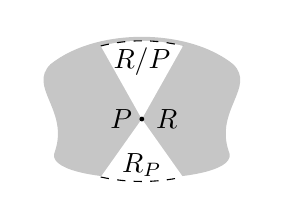
\begin{tikzpicture}[scale=.58]
\fill[gray!45] (-2,1.2) .. controls (-1,2) and (1,2) .. (2,1.2)
.. controls (2.5,.7) and (1.6,.2) .. (1.9,-.7)
.. controls (2.3,-1.5) and (-2.3,-1.5) .. (-1.9,-.7)
.. controls (-1.6,.2) and (-2.5,.7) .. cycle;
\fill[white] (0,0) -- (-.9,1.6) .. controls (-.3,1.75) and (.3,1.75) .. (.9,1.6) -- cycle;
\fill[white] (0,0) -- (-.9,-1.27) .. controls (-.3,-1.4) and (.3,-1.4) .. (.9,-1.27) -- cycle;
\draw[dashed] (-.9,1.6) .. controls (-.3,1.75) and (.3,1.75) .. (.9,1.6);
\draw[dashed] (-.9,-1.27) .. controls (-.3,-1.4) and (.3,-1.4) .. (.9,-1.27);
\fill (0,0) circle (1.5pt);
\node[left] at (0,0) {$P$};\node[right] at (.1,0) {$\Spec R$};
\node at (0,1.25) {$\Spec R/P$};\node at (0,-1) {$\Spec R_P$};
\end{tikzpicture}
\end{center}你能解释这幅图吗?} [\ref{ex:local-vanish}, \ref{ex:pid-localization-dvr}, VI.\ref{ex:local-direct-summand}, VII.\ref{ex:germs-localization}, VIII.\ref{ex:flat-local}]
\end{prob}

\begin{prob}
\label{ex:local-vanish}
$\neg$ (记号如习题~\ref{ex:local-ring}.) 设 $R$ 是交换环, $M$ 是 $R$-模. 证明以下条件等价\footnote{这类结果的理解方式是: $R$ 上的模 $M$ 为零, 当且仅当它在 $\Spec R$ 的每一点处为零. 在局部化 $M_\mathfrak{p}$ 中工作相当于在点 $\mathfrak{p}$ 附近观察; 这就是局部化中的``局部''之意. 如本题所示, 我们常可逐点作局部观察来检测整体性质.}:
\begin{itemize}
\item $M=0$.
\item 对每个素理想 $\mathfrak{p}$ 有 $M_\mathfrak{p}=0$.
\item 对每个极大理想 $\mathfrak{m}$ 有 $M_\mathfrak{m}=0$.
\end{itemize}
(提示: 对有趣的蕴含, 设 $m\in M$ 且 $m\neq0$; 则理想 $\{r\in R\mid rm=0\}$ 是真理想. 由命题~\ref{prop:maximal-ideal-exists}, 它包含于一个极大理想 $\mathfrak{m}$. 关于 $M_\mathfrak{m}$ 你能说什么?) [VIII.\ref{ex:localization-faithfully-exact}, VIII.\ref{ex:flat-local}]
\end{prob}

\begin{prob}
\label{ex:pid-localization-dvr}
$\neg$ 设 $k$ 是域, $v$ 是 $k$ 上的离散赋值. 设 $R$ 是对应的 DVR, 带有局部参数 $t$ (参见习题~\ref{ex:dvr-pid-localparam}).
\begin{itemize}
\item 证明 $R$ 是局部的 (习题~\ref{ex:local-ring}), 极大理想 $\mathfrak{m}=(t)$. (提示: 注意 $R\setminus\mathfrak{m}$ 的每个元素都可逆.)
\item 证明 $k$ 是 $R$ 的分式域.
\item 现在设 $A$ 是 PID, $\mathfrak{p}$ 是 $A$ 中的非零素理想\erratumfootnote{根据官方勘误, 补充 $\mathfrak{p}$ 为非零素理想 (nonzero prime ideal).}. 证明局部化 $A_\mathfrak{p}$ (参见习题~\ref{ex:local-ring}) 是一个 DVR. (提示: 若 $\mathfrak{p}=(p)$, 用``被 $p$ 整除性''在 $A$ 的分式域上定义一个赋值.)
\end{itemize}
[VII.\ref{ex:cusp-coordinate-rings}]
\end{prob}

\begin{prob}
\label{ex:localization-noeth}
用习题~\ref{ex:localization-module} 的记号, 对子模 $N\subseteq M$, $\widehat N\subseteq S^{-1}M$, 分别仿照习题~\ref{ex:localization-ideals} 中定义的运算定义 $N\mapsto N^e$ 与 $\widehat N\mapsto\widehat N^c$. 证明 $(\widehat N^c)^e=\widehat N$. 证明 Noether 模的每个局部化都是 Noether 的.

\noindent 特别地, Noether 环的每个局部化 $S^{-1}R$ 都是 Noether 的.
\end{prob}

\begin{prob}
\label{ex:localization-ufd}
$\neg$ 设 $R$ 是 UFD, $S$ 是 $R$ 的乘闭子集 (参见习题~\ref{ex:localization-ring}).
\begin{itemize}
\item 证明若 $q$ 在 $R$ 中不可约, 则 $q/1$ 在 $S^{-1}R$ 中要么不可约要么为单位.
\item 证明若 $a/s$ 在 $S^{-1}R$ 中不可约, 则 $a/s$ 与某个 $R$ 的不可约元 $q$ 的相伴元 $q/1$ 相伴.
\item 证明 $S^{-1}R$ 也是 UFD.
\end{itemize}
[\ref{ex:ufd-local-criterion}]
\end{prob}

\begin{prob}
\label{ex:ufd-local-criterion}
设 $R$ 是 Noether 整环, $s\in R$, $s\neq 0$, 是素元. 考虑乘闭子集 $S=\{1,s,s^2,\dots\}$. 证明 $R$ 是 UFD, 当且仅当 $S^{-1}R$ 是 UFD. (提示: 由习题~\ref{ex:krull-hauptidealsatz}, 只需证明每个高度为 $1$ 的素理想都主. 用习题~\ref{ex:localization-prime-bijection} 把 $R$ 中的素理想与局部化中的素理想联系起来.)

\noindent 基于诸如本题与习题~\ref{ex:localization-ufd} 的结果, 人们可能猜想``析因'' (factorial) 是一个局部性质, 也就是说, $R$ 是 UFD 当且仅当对所有素理想 $\mathfrak{p}$ 有 $R_\mathfrak{p}$ 是 UFD, 当且仅当对所有极大理想 $\mathfrak{m}$ 有 $R_\mathfrak{m}$ 是 UFD. 遗憾的是情况并非如此. 环 $R$ 若对所有极大理想 $\mathfrak{m}$ 有 $R_\mathfrak{m}$ 是 UFD, 则称为\emph{局部析因的}\index{jubu-kefenjie@局部析因(locally factorial)}; 由习题~\ref{ex:localization-ufd} 析因蕴含局部析因, 但存在不是析因的局部析因环.
\end{prob}

\begin{prob}
\label{ex:prime-subfield}
$\triangleright$ 设 $F$ 是域, 回想环的\emph{特征}\index{tezheng@特征(characteristic)}的概念 (定义~III.\ref{def:characteristic}); 域的特征要么是 $0$ 要么是一个素整数 (习题~III.\ref{ex:characteristic-prime}).
\begin{itemize}
\item 证明 $F$ 特征为 $0$, 当且仅当它包含 $\Q$ 的一个拷贝; 而 $F$ 特征为 $p$, 当且仅当它包含域 $\Z/p\Z$ 的一个拷贝.
\item 证明 (两种情形) 这决定了 $F$ 的最小子域; 它称为 $F$ 的\emph{素子域}\index{suziyu@素子域(prime subfield)}.
\end{itemize}
[§\ref{subsec:adding-roots}, §VII.\ref{subsec:basic-defs}]
\end{prob}

\begin{prob}
\label{ex:units-poly}
$\neg$ 设 $R$ 是整环. 证明 $R[x]$ 中的可逆元恰是视常多项式看的 $R$ 的单位. [\ref{ex:unit-poly-general}]
\end{prob}

\begin{prob}
\label{ex:nilpotent-unit}
$\triangleright$ 环中的元素 $a$ 称为\emph{幂零}\index{miling@幂零(nilpotent)}的, 如果存在 $n\ge 0$ 使得 $a^n=0$. 证明若 $a$ 幂零, 则 $1+a$ 在 $R$ 中是单位. [VI.\ref{ex:nilpotent-matrices}, §VII.\ref{subsec:affine-geometry}]
\end{prob}

\begin{prob}
\label{ex:unit-poly-general}
如下推广习题~\ref{ex:units-poly} 的结果: 设 $R$ 是交换环, $f=a_0+a_1x+\cdots+a_dx^d\in R[x]$; 证明 $f$ 在 $R[x]$ 中是单位, 当且仅当 $a_0$ 在 $R$ 中是单位且 $a_1,\dots,a_d$ 幂零. (提示: 若 $b_0+b_1x+\cdots+b_ex^e$ 是 $f$ 的逆, 用归纳证明对所有 $i\ge 0$ 有 $a_d^{i+1}b_{e-i}=0$, 并推出 $a_d$ 幂零.)
\end{prob}

\begin{prob}
\label{ex:cor4-17}
$\triangleright$ 确立推论~\ref{cor:irreducible-poly-equiv} 中给出的关于 UFD 上不可约多项式的刻画. [§\ref{subsec:ufd-poly}]
\end{prob}

\begin{prob}
\label{ex:common-factor-kxy}
设 $k$ 是域, $f,g$ 是 $k[x,y]=k[x][y]$ 中的两个多项式. 证明若 $f$ 与 $g$ 在 $k(x)[y]$ 中有非平凡公因子, 则它们在 $k[x,y]$ 中有非平凡公因子.
\end{prob}

\begin{prob}
\label{ex:poly-split-rx}
$\triangleright$ 设 $R$ 是 UFD, $K$ 是其分式域, $f(x)\in R[x]$, 并假设 $f(x)=\alpha(x)\beta(x)$ 其中 $\alpha(x),\beta(x)\in K[x]$. 证明存在 $c\in K$ 使得 $c\alpha(x)\in R[x]$, $c^{-1}\beta(x)\in R[x]$, 从而
\[
f(x) = \bigl(c\alpha(x)\bigr)\bigl(c^{-1}\beta(x)\bigr)
\]
把 $f(x)$ 分解为 $R[x]$ 中因子的乘积.

\noindent 推出若 $\alpha(x)\beta(x)=f(x)\in R[x]$ 首一, 且 $\alpha(x)\in K[x]$ 首一, 则 $\alpha(x),\beta(x)$ 都在 $R[x]$ 中且 $\beta(x)$ 也首一. [§\ref{subsec:ufd-poly}, \ref{ex:localization-coeff-product}, §VII.\ref{subsec:cyclotomic}]
\end{prob}

\begin{prob}
\label{ex:localization-coeff-product}
在与习题~\ref{ex:poly-split-rx} 相同的情形中, 证明 $\alpha$ 的任一系数与 $\beta$ 的任一系数的乘积落在 $R$ 中.
\end{prob}

\begin{prob}
\label{ex:fermat-poly}
对多项式证明 Fermat 大定理: 方程
\[
f^n+g^n=h^n
\]
在 $\CC[t]$ 中对 $n>2$ 且 $f,g,h$ 互素且不全为常数时无解\erratumfootnote{根据官方勘误, 明确条件为 $f,g,h$ 互素且不全为常数.}. (提示: 多项式 $1-t^n$ 在 $\CC[t]$ 中分解为 $\prod_{i=1}^{n}(1-\zeta^i t)$, 其中 $\zeta=e^{2\pi i/n}$; 推出 $f^n=\prod_{i=1}^{n}(h-\zeta^i g)$\erratumfootnote{根据官方勘误, 提示中方程修正为 $f^n = \prod_{i=1}^n (h-\zeta^i g)$ (原书曾误印为 $h-g^n$).}. 用 $\CC[t]$ 中的唯一分解得出结论: 每个因子 $h-\zeta^i g$ 都是 $n$ 次幂. 现在令 $h-g=a^n$, $h-\zeta g=b^n$, $h-\zeta^2 g=c^n$ (这里就是 $n>2$ 假设起作用的地方). 用此得到一个关系 $(\lambda a)^n+(\mu b)^n=(\nu c)^n$, 其中 $\lambda,\mu,\nu$ 是适当的复数. 这有什么问题?)

\noindent 同样的证明模式在任何有唯一分解的环境中都行得通; 如果给 $\Z$ 添上一个本原 $n$ 次单位根以及此论证中需要的其他元素的根\erratumfootnote{根据官方勘误, 原书补充说明还需添加论证所需的其他元素的根 (and roots of other elements as needed in this argument).}就得到一个唯一分解整环, 那么完整版的 Fermat 大定理就会像本题指示的那样容易证明. 事实并非如此, 这个事实被 G. Lam\'e 在 1847 年 3 月 1 日向巴黎科学院宣布 Fermat 大定理的一个``证明''时著名地忽略了.
\end{prob}
\section{多项式的不可约性}
\label{sec:poly-irreducibility}

我们在 \S\ref{subsec:ufd-poly}（尤其是推论~\ref{cor:irreducible-poly-equiv}）中的工作, 把 UFD 上多项式的不可约性与相应分式域上多项式的不可约性联系了起来. 例如, $\Z[x]$ 中多项式的不可约性与 $\Q[x]$ 中``本质上是同一回事''. 只要我们有办法有效地验证某一类环或另一类环上多项式的不可约性, 这便能在两个方向上都派上用场. 我们在此汇集若干注记, 旨在判定给定多项式是否不可约, 并简要讨论代数闭域的概念.

\subsection{根与可约性}
\label{subsec:roots-reducibility}

设 $R$ 是环, $f\in R[x]$. 元素 $a\in R$ 称为 $f$ 的\emph{根}, 如果 $f(a)=0$. 回想 (例~III.\ref{ex:linear-monic}) 多项式 $f(x)\in R[x]$ 被 $(x-a)$ 整除, 当且仅当 $a$ 是 $f$ 的根. 更一般地, 我们说 $a$ 是 $f$ 的\emph{$r$ 重根}, 如果 $(x-a)^r$ 整除 $f$ 而 $(x-a)^{r+1}$ 不整除 $f$. 读者大概从微积分的经验中熟悉这个概念. 例如, 在原点处分别有 $1,2,3$ 重根的多项式的图像（在原点附近）看起来就像

\begin{center}
\begin{tikzpicture}[scale=.8]
\begin{scope}[shift={(-3,0)}]
\draw[gray] (-1.1,0)--(2.2,0);
\draw[gray] (0,-1.1)--(0,2.1);
\clip (-1.1,-1.1) rectangle (2.2,2.1);
\draw[thick] plot[smooth] coordinates {(-1.1000,1.9305) (-1.0670,1.8497) (-1.0340,1.7703) (-1.0010,1.6923) (-0.9680,1.6158) (-0.9350,1.5406) (-0.9020,1.4669) (-0.8690,1.3946) (-0.8360,1.3237) (-0.8030,1.2542) (-0.7700,1.1862) (-0.7370,1.1195) (-0.7040,1.0543) (-0.6710,0.9905) (-0.6380,0.9281) (-0.6050,0.8671) (-0.5720,0.8075) (-0.5390,0.7494) (-0.5060,0.6927) (-0.4730,0.6373) (-0.4400,0.5834) (-0.4070,0.5310) (-0.3740,0.4799) (-0.3410,0.4302) (-0.3080,0.3820) (-0.2750,0.3352) (-0.2420,0.2897) (-0.2090,0.2458) (-0.1760,0.2032) (-0.1430,0.1620) (-0.1100,0.1223) (-0.0770,0.0839) (-0.0440,0.0470) (-0.0110,0.0115) (0.0220,-0.0226) (0.0550,-0.0552) (0.0880,-0.0865) (0.1210,-0.1163) (0.1540,-0.1447) (0.1870,-0.1718) (0.2200,-0.1973) (0.2530,-0.2215) (0.2860,-0.2443) (0.3190,-0.2656) (0.3520,-0.2855) (0.3850,-0.3041) (0.4180,-0.3211) (0.4510,-0.3368) (0.4840,-0.3511) (0.5170,-0.3639) (0.5500,-0.3754) (0.5830,-0.3854) (0.6160,-0.3940) (0.6490,-0.4012) (0.6820,-0.4069) (0.7150,-0.4113) (0.7480,-0.4142) (0.7810,-0.4158) (0.8140,-0.4159) (0.8470,-0.4146) (0.8800,-0.4118) (0.9130,-0.4077) (0.9460,-0.4021) (0.9790,-0.3952) (1.0120,-0.3868) (1.0450,-0.3770) (1.0780,-0.3658) (1.1110,-0.3531) (1.1440,-0.3391) (1.1770,-0.3236) (1.2100,-0.3067) (1.2430,-0.2884) (1.2760,-0.2687) (1.3090,-0.2476) (1.3420,-0.2251) (1.3750,-0.2011) (1.4080,-0.1757) (1.4410,-0.1489) (1.4740,-0.1207) (1.5070,-0.0911) (1.5400,-0.0601) (1.5730,-0.0276) (1.6060,0.0063) (1.6390,0.0415) (1.6720,0.0782) (1.7050,0.1164) (1.7380,0.1559) (1.7710,0.1968) (1.8040,0.2392) (1.8370,0.2830) (1.8700,0.3282) (1.9030,0.3748) (1.9360,0.4228) (1.9690,0.4723) (2.0020,0.5231) (2.0350,0.5754) (2.0680,0.6291) (2.1010,0.6842) (2.1340,0.7407) (2.1670,0.7986) (2.2000,0.8580)};
\end{scope}
\begin{scope}[shift={(3,0)}]
\draw[gray] (-1.1,0)--(2.2,0);
\draw[gray] (0,-1.1)--(0,2.1);
\clip (-1.1,-1.1) rectangle (2.2,2.1);
\draw[thick] plot[smooth] coordinates {(-1.1000,2.1236) (-1.0670,1.9736) (-1.0340,1.8305) (-1.0010,1.6940) (-0.9680,1.5641) (-0.9350,1.4405) (-0.9020,1.3232) (-0.8690,1.2119) (-0.8360,1.1066) (-0.8030,1.0072) (-0.7700,0.9134) (-0.7370,0.8251) (-0.7040,0.7422) (-0.6710,0.6646) (-0.6380,0.5921) (-0.6050,0.5246) (-0.5720,0.4619) (-0.5390,0.4039) (-0.5060,0.3505) (-0.4730,0.3015) (-0.4400,0.2567) (-0.4070,0.2161) (-0.3740,0.1795) (-0.3410,0.1467) (-0.3080,0.1177) (-0.2750,0.0922) (-0.2420,0.0701) (-0.2090,0.0514) (-0.1760,0.0358) (-0.1430,0.0232) (-0.1100,0.0134) (-0.0770,0.0065) (-0.0440,0.0021) (-0.0110,0.0001) (0.0220,0.0005) (0.0550,0.0030) (0.0880,0.0076) (0.1210,0.0141) (0.1540,0.0223) (0.1870,0.0321) (0.2200,0.0434) (0.2530,0.0560) (0.2860,0.0699) (0.3190,0.0847) (0.3520,0.1005) (0.3850,0.1171) (0.4180,0.1342) (0.4510,0.1519) (0.4840,0.1699) (0.5170,0.1882) (0.5500,0.2065) (0.5830,0.2247) (0.6160,0.2427) (0.6490,0.2604) (0.6820,0.2775) (0.7150,0.2941) (0.7480,0.3099) (0.7810,0.3247) (0.8140,0.3385) (0.8470,0.3511) (0.8800,0.3624) (0.9130,0.3722) (0.9460,0.3804) (0.9790,0.3869) (1.0120,0.3914) (1.0450,0.3939) (1.0780,0.3943) (1.1110,0.3923) (1.1440,0.3879) (1.1770,0.3809) (1.2100,0.3711) (1.2430,0.3585) (1.2760,0.3429) (1.3090,0.3241) (1.3420,0.3020) (1.3750,0.2765) (1.4080,0.2474) (1.4410,0.2146) (1.4740,0.1779) (1.5070,0.1373) (1.5400,0.0925) (1.5730,0.0434) (1.6060,-0.0101) (1.6390,-0.0681) (1.6720,-0.1308) (1.7050,-0.1984) (1.7380,-0.2710) (1.7710,-0.3486) (1.8040,-0.4315) (1.8370,-0.5199) (1.8700,-0.6137) (1.9030,-0.7132) (1.9360,-0.8186) (1.9690,-0.9299) (2.0020,-1.0473) (2.0350,-1.1709) (2.0680,-1.3009) (2.1010,-1.4375) (2.1340,-1.5807) (2.1670,-1.7307) (2.2000,-1.8876)};
\end{scope}
\begin{scope}[shift={(0,-4)}]
\draw[gray] (-1.1,0)--(2.2,0);
\draw[gray] (0,-1.1)--(0,2.1);
\clip (-1.1,-1.1) rectangle (2.2,2.1);
\draw[thick] plot[smooth] coordinates {(-1.1000,2.3359) (-1.0670,2.1059) (-1.0340,1.8927) (-1.0010,1.6957) (-0.9680,1.5140) (-0.9350,1.3469) (-0.9020,1.1935) (-0.8690,1.0532) (-0.8360,0.9251) (-0.8030,0.8087) (-0.7700,0.7033) (-0.7370,0.6081) (-0.7040,0.5225) (-0.6710,0.4460) (-0.6380,0.3778) (-0.6050,0.3174) (-0.5720,0.2642) (-0.5390,0.2177) (-0.5060,0.1773) (-0.4730,0.1426) (-0.4400,0.1130) (-0.4070,0.0880) (-0.3740,0.0671) (-0.3410,0.0500) (-0.3080,0.0362) (-0.2750,0.0253) (-0.2420,0.0170) (-0.2090,0.0107) (-0.1760,0.0063) (-0.1430,0.0033) (-0.1100,0.0015) (-0.0770,0.0005) (-0.0440,0.0001) (-0.0110,0.0000) (0.0220,-0.0000) (0.0550,-0.0002) (0.0880,-0.0007) (0.1210,-0.0017) (0.1540,-0.0034) (0.1870,-0.0060) (0.2200,-0.0096) (0.2530,-0.0142) (0.2860,-0.0200) (0.3190,-0.0270) (0.3520,-0.0354) (0.3850,-0.0451) (0.4180,-0.0561) (0.4510,-0.0685) (0.4840,-0.0822) (0.5170,-0.0973) (0.5500,-0.1136) (0.5830,-0.1310) (0.6160,-0.1495) (0.6490,-0.1690) (0.6820,-0.1893) (0.7150,-0.2103) (0.7480,-0.2318) (0.7810,-0.2536) (0.8140,-0.2756) (0.8470,-0.2974) (0.8800,-0.3189) (0.9130,-0.3398) (0.9460,-0.3599) (0.9790,-0.3788) (1.0120,-0.3961) (1.0450,-0.4117) (1.0780,-0.4251) (1.1110,-0.4359) (1.1440,-0.4438) (1.1770,-0.4483) (1.2100,-0.4491) (1.2430,-0.4457) (1.2760,-0.4375) (1.3090,-0.4243) (1.3420,-0.4053) (1.3750,-0.3802) (1.4080,-0.3484) (1.4410,-0.3092) (1.4740,-0.2623) (1.5070,-0.2069) (1.5400,-0.1424) (1.5730,-0.0683) (1.6060,0.0162) (1.6390,0.1116) (1.6720,0.2188) (1.7050,0.3383) (1.7380,0.4709) (1.7710,0.6174) (1.8040,0.7785) (1.8370,0.9550) (1.8700,1.1476) (1.9030,1.3573) (1.9360,1.5848) (1.9690,1.8310) (2.0020,2.0967) (2.0350,2.3828) (2.0680,2.6904) (2.1010,3.0202) (2.1340,3.3732) (2.1670,3.7504) (2.2000,4.1527)};
\end{scope}
\end{tikzpicture}
\end{center}

\begin{lemma}\label{lem:roots-count}
设 $R$ 是整环, $f\in R[x]$ 是 $n$ 次多项式. 则 $f$ 的根的个数（计重数）至多为 $n$.
\end{lemma}

\begin{proof}
$f$ 在 $R$ 中的根的个数小于或等于把 $f$ 视作其分式域 $K$ 上的多项式时根的个数; 因此我们可以用 $K$ 代替 $R$.

现在 $K[x]$ 是 UFD, 而 $f$ 的根对应于 $f$ 的 $1$ 次不可约因子. 由于 $f$ 的所有不可约因子的乘积次数为 $n$, 故 $1$ 次因子的个数至多为 $n$, 证毕.
\end{proof}

值得记住这个证明中用到的把整环 $R$ 替换为它的分式域 $K$ 的技巧: 人们常常能利用 $K$ 是域所带来的便利性质（此例中即 $K[x]$ 是 UFD）, 即便 $R$ 离满足这种性质相差甚远（$R[x]$ 未必是 UFD, 因为 $R$ 自身未必是 UFD）.

还要注意, 若 $R$ 不是整环, 引理~\ref{lem:roots-count} 的结论可能不成立. 例如, 二次多项式 $x^2+x$ 在 $\Z/6\Z$ 上有四个根.

这个看似平凡的引理~\ref{lem:roots-count} 有着重要的应用: 例如我们在定理~IV.\ref{thm:finite-subfield-cyclic} 的证明中（不事声张地）用到过它. 此外, 回想多项式 $f\in R[x]$ 决定了一个``求值函数''（参见例~III.\ref{ex:extension-property}）$R\to R$, 即 $r\mapsto f(r)$. 读者在习题~III.\ref{ex:poly-function} 中验证过, 一般说来这个函数并不决定多项式; 但在无限整环上, 多项式由相应的函数决定:

\begin{corollary}\label{cor:eval-func-detect}
设 $R$ 是无限整环, $f,g\in R[x]$ 是多项式. 则 $f=g$, 当且仅当求值函数 $r\mapsto f(r)$, $r\mapsto g(r)$ 一致.
\end{corollary}

\begin{proof}
的确, 这两个函数一致, 当且仅当每个 $a\in R$ 都是 $f-g$ 的根; 但由引理~\ref{lem:roots-count}, $R$ 上的非零多项式不可能有无限多个根.
\end{proof}

显然, 次数 $\geq 2$ 的不可约多项式不可能有根. 对于域上的 $2$ 次和 $3$ 次多项式, 逆命题也成立:

\begin{proposition}\label{prop:irred-deg2-3}
设 $k$ 是域. $f\in k[x]$ 是 $2$ 次或 $3$ 次多项式, 则 $f$ 不可约, 当且仅当它没有根.
\end{proposition}

\begin{proof}
习题~\ref{ex:prove-prop5.3}.
\end{proof}

\begin{example}\label{ex:f2-field4}
设 $\F_2$ 是域 $\Z/2\Z$.

多项式 $f(t)=t^2+t+1\in\F_2[t]$ 不可约, 因为它没有根: $f(0)=f(1)=1$. 因此理想 $(t^2+t+1)$ 在 $\F_2[t]$ 中是素的, 从而是极大的（因为 $\F_2[t]$ 是 PID: 别忘了命题~III.\ref{prop:PID-prime-maximal}). 这就给出了一秒钟构造一个有四个元素的域:
\[
\frac{\F_2[t]}{(t^2+t+1)}.
\]
\index{yu@域(field)!fenyuan@分圆(cyclotomic)}读者（但愿）在习题~III.\ref{ex:field-4-elements} 中通过手工寻找合适的乘法表这一繁琐过程构造过这个域. 读者现在要构造大得多的例子应该毫无困难（参见习题~\ref{ex:fields-27-121}）.
\end{example}

命题~\ref{prop:irred-deg2-3} 很悦人, 也能帮助判定更一般环上的不可约性: 例如, $\Z[x]$ 中 $2$ 次或 $3$ 次的本原多项式 $f$ 不可约, 当且仅当它在 $\Q$ 中没有根. 的确, $f$ 在 $\Z[x]$ 中不可约, 当且仅当它在 $\Q[x]$ 中不可约（由推论~\ref{cor:irreducible-poly-equiv}）. 不过要注意, 例如 $4x^2-1=(2x-1)(2x+1)$ 是本原的且在 $\Z[x]$ 中可约, 尽管它没有整数根. 还要记住, 命题~\ref{prop:irred-deg2-3} 的结论对次数 $\geq 4$ 的多项式可能不成立: 例如 $x^4+2x^2+1=(x^2+1)^2$ 在 $\Q[x]$ 中可约, 但它没有有理根.

在 $\Z[x]$ 中寻找多项式的有理根, 原则上是一个有限的过程, 这源于以下的观察（它在每个 UFD 上都成立）. 这通常称为``有理根检验''.

\begin{proposition}[有理根检验]\label{prop:rational-root-test}
设 $R$ 是 UFD, $K$ 是它的分式域. 设
\[
f(x)=a_0+a_1x+\cdots+a_nx^n\in R[x],
\]
并设 $c=\frac{p}{q}\in K$ 是 $f$ 的根, 其中 $p,q\in R$, $\gcd(p,q)=1$. 则 $p\mid a_0$ 且 $q\mid a_n$ （在 $R$ 中）.
\end{proposition}

\begin{proof}
由假设,
\[
a_0+a_1\frac{p}{q}+\cdots+a_n\frac{p^n}{q^n}=0;
\]
也就是说,
\[
a_0q^n+a_1pq^{n-1}+\cdots+a_np^n=0.
\]
因此
\[
a_0q^n=-p(a_1q^{n-1}+\cdots+a_np^{n-1}),
\]
这就证明 $p\mid (a_0q^n)$. 由于 $p$ 与 $q$ 的最大公因是 $1$, 这意味着 $p$ 的不可约因子（作为多重集）都包含在 $a_0$ 的不可约因子之中, 即 $p\mid a_0$.

完全类似的论证证明 $q\mid a_n$.
\end{proof}

\begin{example}\label{ex:rational-roots-poly}
\index{duoxiangshi@多项式(polynomial)!fenyuan@分圆(cyclotomic)}寻找多项式
\[
3-2x+3x^2-2x^3+3x^4-2x^5
\]
的有理根, 于是就归结为试一试形如 $\frac{p}{q}$ 的分数, 其中 $q=\pm1,\pm2$, $p=\pm1,\pm3$. 结果, $\frac{3}{2}$ 是这些可能中发现的唯一根, 由此可知它就是该多项式唯一的有理根.
\end{example}

\subsection{添加根; 代数闭域}
\label{subsec:adding-roots}

\index{yu@域(field)!kuozhang@扩张(extension)}域的同态
\[
i:k\to F
\]
必然是单的（参见习题~III.\ref{ex:field-to-ring}）: 的确, 它的核是 $k$ 的真理想, 而域的唯一真理想是 $(0)$. 在这种情形下, 我们说 $F$（更恰当地说是同态 $i$）是 $k$ 的一个\emph{扩张}. 略为滥用语言, 我们便把 $k$ 想成包含在 $F$ 中: $k\subseteq F$. 要记住, 只要存在任何一个环同态 $k\to F$, 情形就是如此.

\index{yu@域(field)!youxian@有限(finite)}有一个构造扩张的标准程序, 使得某个给定多项式在其中获得一个根; 我们在例~III.\ref{ex:C-from-R} 中遇到过这个过程的一个实例. 事实上, 这样得到的域相对于这个要求几乎是泛的.

\begin{proposition}\label{prop:adjoin-root}
设 $k$ 是域, $f(t)\in k[t]$ 是非零不可约多项式. 则
\[
F:=\frac{k[t]}{(f(t))}
\]
是一个域, 带有自然同态 $i:k\hookrightarrow F$（作为复合 $k\to k[x]\to F$）, 使之成为 $k$ 的扩张. 进一步,
\begin{itemize}
\item $f(x)\in k[x]\subseteq F[x]$ 在 $F$ 中有一个根, 即 $t$ 的陪集;
\item 若 $k\subseteq K$ 是 $f$ 有根的任一扩张, 则存在同态 $j:F\to K$ 使得下图交换:
\end{itemize}
\[
\begin{tikzcd}
k \arrow[r, hook, "i"] \arrow[dr,hook] & F \arrow[d,hook, "j"] \\
& K
\end{tikzcd}
\]
\end{proposition}

\begin{proof}
由于 $k$ 是域, $k[t]$ 是 PID; 因此由命题~III.\ref{prop:PID-prime-maximal}, $(f(t))$ 是 $k[t]$ 的极大理想. 从而 $F$ 确为域. 把 $k[t]/(f(t))=F$ 中的陪集用加下划线表示, 我们有
\[
f(\underline{t})=\underline{f(t)}=0,
\]
如宣称的那样.

为验证陈述的第二部分, 设 $k\subseteq K$ 是扩张且 $f(u)=0$, 其中 $u\in K$. 这意味着求值同态
\[
\epsilon:k[t]\to K
\]
（由 $\epsilon(g(t)):=g(u)$ 定义）在 $f(t)$ 处取值为 $0$; 因此 $(f(t))\subseteq\ker(\epsilon)$, 而商的泛性质给出唯一的同态
\[
j:F=\frac{k[t]}{(f(t))}\to K
\]
满足所陈述的要求.
\end{proof}

我们止步于宣称命题~\ref{prop:adjoin-root} 构造的扩张相对于``含有 $f$ 的一个根''这个要求是泛的, 因为陈述中出现的同态 $j$ 并不唯一: 事实上, 证明表明这样的同态的个数等于 $f$ 在更大的域 $K$ 中根的个数. 我们不妨说 $F$ 是\emph{泛的}（versal, 意为``不具有唯一性的 universal''）. 如果我们把 $f$ 的根的信息也包含进来, 就能得到完全的泛性; 我们将在第七章分析域扩张时回到这个构造.

\begin{example}\label{ex:adjoin-root-C}
取 $k=\R$ 且 $f(x)=x^2+1$, 命题~\ref{prop:adjoin-root} 构造的域（同构于）$\CC$: 这在例~III.\ref{ex:C-from-R} 中已被仔细验证过.

类似地, $\Q[t]/(t^2-2)$ 给出一个含有 $\Q$ 且其中有``$2$ 的平方根''的域. 这个域在 $\R$ 中有两个嵌入, 因为 $\R$ 含有 $2$ 的两个不同平方根: $\pm\sqrt{2}$.
\end{example}

命题~\ref{prop:adjoin-root} 构造的扩张 $F$ 中, 不可约多项式 $f\in k[x]$ 获得了一个根, 这意味着 $f$ 在 $F$ 上有一个线性（即 $1$ 次）因子; 特别地, 若 $\deg(f)>1$, 则 $f$ 在 $F$ 上不再是不可约的.

给定任意多项式 $f\in k[x]$, 很容易构造 $k$ 的一个扩张, 使得 $f$ 在其中完全分解为线性因子的乘积（习题~\ref{ex:splitting-extension}). 对每个非零 $f$ 这已经在 $k$ 自身中发生的情况非常重要, 因此给它一个名字.

\begin{definition}\label{def:alg-closed}
域 $k$ 称为\emph{代数闭}的, 如果 $k[x]$ 中所有不可约多项式的次数都是 $1$.
\end{definition}

我们在前面的例~III.\ref{ex:spec-kx}（以及习题~III.\ref{ex:closed-maximal}）中顺带遇到过这个概念. 下面的引理留给读者:

\begin{lemma}\label{lem:alg-closed-chars}
域 $k$ 是代数闭的, 当且仅当每个非常数多项式 $f\in k[x]$ 都完全分解为线性因子的乘积, 当且仅当每个非常值多项式 $f\in k[x]$ 在 $k$ 中都有根.
\end{lemma}

\index{zhu@柱(cylinder)}换言之, 域 $k$ 是代数闭的, 当且仅当系数在 $k$ 中且没有解的多项式方程只有``$0$ 次''的方程, 例如 $1=0$. 称为 Nullstellensatz（零点定理）的结果（也归功于 David Hilbert; 我们在第三章提到过）是这个观察的极大推广, 也是（老式）代数几何的支柱之一. 我们将在 \S VII.\ref{sec:alg-closure-nullstellensatz} 回到这一切.

我们遇到的有限域（例如对素数 $p$ 的 $\Z/p\Z$）中有代数闭的吗? 没有. 改造 Euclid 证明素数有无穷多个的论证（习题~\ref{ex:infinitely-many-primes}）表明, 代数闭域都是无限的.

\begin{proposition}\label{prop:alg-closed-infinite}
设 $k$ 是代数闭域. 则 $k$ 是无限的.
\end{proposition}

\begin{proof}
反证. 设 $k$ 代数闭且有限; 记 $k$ 的元素为 $c_1,\ldots,c_N$.

则在 $k[x]$ 中恰有 $N$ 个首一不可约多项式, 即 $(x-c_1),\ldots,(x-c_N)$. 考虑多项式
\[
f(x)=(x-c_1)\cdots(x-c_N)+1:
\]
对所有 $c\in k$ 我们有
\[
f(c)=(c-c_1)\cdots(c-c_N)+1=1\neq 0,
\]
因为 $c$ 等于某个 $c_i$. 于是 $f(x)$ 是一个没有根的非常数多项式, 与引理~\ref{lem:alg-closed-chars} 矛盾.
\end{proof}

既然有限域不是代数闭的, 读者可能会怀疑代数闭域必然特征为 $0$（参见习题~\ref{ex:prime-subfield}). 事实并非如此: 任何特征的代数闭域都存在. 的确, 正如我们适时将会看到的, 每个域 $F$ 都可嵌入一个代数闭域; 这种扩张中最小的一个称为 $F$ 的\emph{代数闭包}, 记作 $\overline{F}$. 因此, 例如 $\overline{\Z/2\Z}$ 就是一个特征为 $2$ 的代数闭域.

代数闭包 $\overline{\Q}$ 是 $\CC$ 的一个可数子域. 扩张 $\Q\subseteq\overline{\Q}$, 尤其是它的``Galois 群''（参见 \S VII.\ref{sec:galois-theory}）, 被视为数学中最重要的研究对象之一（参见推论~VII.\ref{cor:every-finite-group-galois} 之后的讨论）.

\index{daishubibao@代数闭包(algebraic closure)!youxianyude@有限域的(of finite fields)}我们将在 \S VII.\ref{subsec:algebraic-closure} 中相当显式地构造一个域的代数闭包.

\subsection{\texorpdfstring{$\mathbb{C}[x]$}{C[x]}、\texorpdfstring{$\mathbb{R}[x]$}{R[x]}、\texorpdfstring{$\mathbb{Q}[x]$}{Q[x]} 中的不可约性}
\label{subsec:irred-CRQ}

每个多项式 $f\in\CC[x]$ 都在 $\CC$ 上完全分解. 的确,

\index{daishu@代数(algebra)!shu@数(number)}\index{daishu@代数(algebra)!jihe@几何(geometry)}\index{daishu@代数(algebra)!kuozhangdeyuan@扩张的元(element of an extension)}\index{daishu@代数(algebra)!bibao@闭包(closure)}\begin{theorem}\label{thm:C-algebraically-closed}
$\CC$ 是代数闭的.
\end{theorem}

\index{Argand@Argand!Jean-Robert@Jean-Robert}\index{Gauss@Gauss!Carl Friedrich@Carl Friedrich}Gauss 被归功于给出了这个基本定理\footnote{实际上, Gauss 的第一个证明显然有漏洞; 第一个严格的证明归于 Argand. 后来 Gauss 弥补了他证明中的漏洞, 并给出了另外几个证明.}（它确实被称为代数基本定理）.

代数基本定理的``代数''证明需要比我们目前所知更多的知识（我们会在 \S VII.\ref{subsec:ft-algebra}, 在学了一点 Galois 理论之后遇到一个）; 说来奇怪, 一点点复分析就使得这个结论几乎显然. 下面是这种论证的一个概要. 设 $f\in\CC[x]$ 是非常数多项式; 任务（参见引理~\ref{lem:alg-closed-chars}）在于证明 $f$ 在 $\CC$ 中有根. 无论 $f(0)$ 是什么, 我们都能取足够大的 $r\in\R$, 使得对圆周 $|z|=r$ 上所有 $z$ 都有 $|f(z)|>|f(0)|$（因为 $f$ 非常值, $\lim_{z\to\infty}|f(z)|=+\infty$）. 圆盘 $|z|\leq r$ 是紧的, 所以连续函数 $|f(z)|$ 在其上取最小值; 由 $r$ 的取法, 这个最小值必在圆盘内部某点, 设为 $z=a$. 最小模原理（参见习题~\ref{ex:min-modulus-principle}）随之给出 $f(a)=0$, 证毕.

由定理~\ref{thm:C-algebraically-closed}, $\CC[x]$ 中多项式的不可约性简单到了极点: $\CC[x]$ 中的非常值多项式 $f$ 不可约, 当且仅当它的次数为 $1$. 每个次数 $\geq 2$ 的 $f\in\CC[x]$ 都是可约的.

在 $\R$ 上, 情形几乎同样简单:

\begin{proposition}\label{prop:irred-R}
每个多项式 $f\in\R[x]$ 若次数 $\geq 3$ 则可约.

$\R[x]$ 中非常值的不可约多项式恰好是 $1$ 次多项式以及二次多项式
\[
f=ax^2+bx+c
\]
其中 $b^2-4ac<0$.
\end{proposition}

\begin{proof}
设 $f\in\R[x]$ 是非常值多项式:
\[
f=a_0+a_1x+\cdots+a_nx^n,
\]
所有 $a_i\in\R$. 由定理~\ref{thm:C-algebraically-closed}, $f$ 有一个复根 $z$:
\[
a_0+a_1z+\cdots+a_nz^n=0.
\]
应用复共轭 $z\mapsto\overline{z}$, 并注意由于 $a_i\in\R$ 有 $\overline{a}_i=a_i$,
\[
a_0+a_1\overline{z}+\cdots+a_n\overline{z}^n
=\overline{a_0}+\overline{a_1}\,\overline{z}+\cdots+\overline{a_n}\,\overline{z}^n
=\overline{a_0+a_1z+\cdots+a_nz^n}=0:
\]
这说明 $\overline{z}$ 也是 $f$ 的根. 有两种可能:
\begin{itemize}
\item 要么 $z=\overline{z}$, 即 $z=r$ 本来就是实数, 于是 $(x-r)$ 是 $f$ 在 $\R[x]$ 中的一个因子; 或者
\item $z\neq\overline{z}$, 此时 $(x-z)$ 与 $(x-\overline{z})$ 是 $f$ 在 $\CC[x]$ 中不相伴的不可约因子. 在这种情形下（因为 $\CC[x]$ 是 UFD!）
\[
x^2-(z+\overline{z})x+z\overline{z}=(x-z)(x-\overline{z})
\]
整除 $f$.
\end{itemize}
由于 $z+\overline{z}$ 与 $z\overline{z}$ 都是实数, 这个分析表明每个非常值 $f\in\R[x]$ 都有一个次数 $\leq 2$ 的不可约因子, 证明了第一个断言.

第二个断言随即由命题~\ref{prop:irred-deg2-3} 以及如下事实推出: $\R[x]$ 中没有实根的二次多项式恰好是形如 $ax^2+bx+c$ 且 $b^2-4ac<0$ 的多项式.
\end{proof}

下面的注记是命题~\ref{prop:irred-R} 的直接推论, 从初等微积分看也显然（习题~\ref{ex:odd-degree-ivt}）:

\begin{corollary}\label{cor:odd-degree-real-root}
每个奇数次的多项式 $f\in\R[x]$ 都有一个实根.
\end{corollary}

\index{Eisenstein@Eisenstein!Ferdinand Gotthold Max@Ferdinand Gotthold Max!panbiefa@判别法(criterion)}\index{Eisenstein@Eisenstein!Ferdinand Gotthold Max@Ferdinand Gotthold Max}总而言之, $\CC[x]$ 或 $\R[x]$ 中多项式的不可约性问题非常直白. 相比之下, $\Q[x]$ 中的不可约性是个复杂的问题: 正如我们所见（命题~\ref{prop:irreducible-over-field}）, 它与 $\Z[x]$ 中的不可约性一样微妙. $\Z[x]$ 中不可约性没有鲜明的刻画; 但下面这些朴素的注记（以及 \S\ref{subsec:eisenstein} 讨论的 Eisenstein 判别法）在许多有趣的情形已经足够.

一个朴素的注记是: 若 $\varphi:R\to S$ 是同态, 且 $a$ 在 $R$ 中可约, 则 $\varphi(a)$ 很可能在 $S$ 中可约. 这仅仅是因为若 $a=bc$, 则 $\varphi(a)=\varphi(b)\varphi(c)$.

当然这并不全然正确: 例如因为 $\varphi(a)$ 和/或 $\varphi(b)$ 和/或 $\varphi(c)$ 在 $S$ 中可能是单位. 但只要对特例多加小心, 这个观察便能发挥巨大作用, 尤其是以其逆否形式: 若 $\varphi(a)$ 在 $S$ 中不可约, 则 $a$ 在 $R$ 中（很可能……）不可约.

下面这个简单的陈述把上述注记形式化, 取 $R=\Z[x]$. 自然投影 $\Z\to\Z/p\Z$ 诱导一个满同态 $\pi:\Z[x]\to\Z/p\Z[x]$: 很简单, $\pi(f)$ 就是把 $f$ 的所有系数模 $p$ 读出所得; 我们把这个操作的结果写作``$f\bmod p$''.

\begin{proposition}\label{prop:mod-p-irred}
设 $f\in\Z[x]$ 是本原多项式, $p$ 是素数. 假设 $f\bmod p$ 与 $f$ 次数相同, 且在 $\Z/p\Z[x]$ 中不可约. 则 $f$ 在 $\Z[x]$ 中不可约.
\end{proposition}

\begin{proof}
用逆否论证: 若 $f$ 本原且在 $\Z[x]$ 中可约, $\deg f=n$, 则 $f=gh$ 其中 $\deg g=d$, $\deg h=e$, $d+e=n$, 且 $d,e$ 皆为正. 但对 $f\bmod p$ 也可说同样的话, 所以 $f\bmod p$ 也可约.
\end{proof}

关于次数的假设是必要的, 正是为了照顾前述讨论中提到的``特例''. 例如 $(2x^3+3x^2+3x+1)$ 等于 $(x^2+x+1)\bmod 2$, 而后者在 $\Z/2\Z[x]$ 中不可约; 然而 $(2x+1)$ 是前者的一个因子. 要点当然是 $2x+1$ 模 $2$ 是一个单位.

警告: 正如我们在相当远的将来（例~VII.\ref{ex:xp1-red}）将会看到的, $\Z[x]$ 中存在这样的不可约多项式, 它们在所有素数模下都可约! 所以命题~\ref{prop:mod-p-irred} 不能变成 $\Z[x]$ 中不可约性的一个刻画. 不过它在产生例子时相当有用. 例如,

\begin{corollary}\label{cor:arbitrary-degree-irred}
在 $\Z[x]$ 与 $\Q[x]$ 中存在任意大次数的不可约多项式.
\end{corollary}

\begin{proof}
由命题~\ref{prop:irreducible-over-field}, 对 $\Z[x]$ 的论断推出对 $\Q[x]$ 的论断. 由命题~\ref{prop:mod-p-irred}, 只需验证对任意素数 $p$, 在 $\Z/p\Z[x]$ 中存在任意大次数的不可约多项式. 这是习题~\ref{ex:finite-field-irred-arbitrary} 的一个特例.
\end{proof}

\subsection{Eisenstein 判别法}
\label{subsec:eisenstein}

我们把这个结果单独放在一小节, 只因为它是非常著名的; 它也和导出命题~\ref{prop:mod-p-irred} 的那些考虑一样朴素, 而且它其实并不是一个``判别法'', 因为它同样没有给出不可约性的一个刻画.

这个结果通常对 $\Z$ 陈述, 但它在每个环 $R$ 上都成立.

\begin{proposition}[Eisenstein 判别法]\label{prop:eisenstein}
设 $R$ 是（交换）环, $\mathfrak{p}$ 是 $R$ 的一个素理想. 设
\[
f=a_0+a_1x+\cdots+a_nx^n\in R[x]
\]
\index{duoxiangshi@多项式(polynomial)!dedaoshu@的导数(derivative of a)}是一个多项式, 并假设
\begin{itemize}
\item $a_n\notin\mathfrak{p}$;
\item $a_i\in\mathfrak{p}$ 对 $i=0,\ldots,n-1$;
\item $a_0\notin\mathfrak{p}^2$.
\end{itemize}
则 $f$ 不是 $R[x]$ 中次数 $<n$ 的多项式的乘积.
\end{proposition}

\begin{proof}
反证. 设 $f=gh$ 在 $R[x]$ 中, 且 $d=\deg g$ 与 $e=\deg h$ 都小于 $n=\deg f$; 写出
\[
g=b_0+b_1x+\cdots+b_dx^d,\qquad h=c_0+c_1x+\cdots+c_ex^e,
\]
并注意必有 $d>0$ 且 $e>0$. 考虑模 $\mathfrak{p}$ 的 $f$: 于是
\[
\underline{f}=\underline{g}\,\underline{h}\quad\text{在 }(R/\mathfrak{p})[x]\text{ 中},
\]
其中 $\underline{f}$ 表示 $f$ 模 $\mathfrak{p}$, 等等.

由假设, 模 $\mathfrak{p}$ 有 $\underline{f}=\underline{a}_nx^n$, 其中 $\underline{a}_n\neq 0$ 在 $R/\mathfrak{p}$ 中. 由于 $R/\mathfrak{p}$ 是整环, $\underline{f}$ 的因子也必为单项: 即必有
\[
\underline{g}=\underline{b}_{d'}x^{d'},\qquad \underline{h}=\underline{c}_{e'}x^{e'},
\]
其中 $d'\le d < n$, $e'\le e < n$\erratumfootnote{根据官方勘误, 严密考虑模 $\mathfrak{p}$ 后的次数 $d'\le d<n, e'\le e<n$; 由 $d'+e'=n$ 得 $d'>0, e'>0$.}. 由于 $d'+e'=n$, 我们有 $d'>0$, $e'>0$, 这推出 $b_0\in\mathfrak{p}$, $c_0\in\mathfrak{p}$.

但于是 $a_0=b_0c_0\in\mathfrak{p}^2$, 与假设矛盾.
\end{proof}

例如, $x^4+2x^2+2$ 必在 $\Z[x]$ 中（从而在 $\Q[x]$ 中）不可约: 取 $R=\Z$, $\mathfrak{p}=(2)$ 应用 Eisenstein 判别法. 更令人兴奋的应用涉及整类的多项式:

\begin{example}\label{ex:xn-minus-p}
对所有 $n$ 与所有素数 $p$, 多项式 $x^n-p$ 在 $\Z[x]$ 中不可约. 这由 Eisenstein 判别法立即得到, 并给出推论~\ref{cor:arbitrary-degree-irred} 的另一个证明.
\end{example}

\index{fenyuan@分圆(cyclotomic)!duoxiangshi@多项式(polynomial)}\index{fenyuan@分圆(cyclotomic)!yu@域(field)}\index{fenyuan@分圆(cyclotomic)}\begin{example}\label{ex:cyclotomic-eisenstein}
这可能是 Eisenstein 判别法最著名的应用. 设 $p$ 是素数, 并设
\[
f(x)=1+x+x^2+\cdots+x^{p-1}\in\Z[x].
\]
这些多项式称为分圆多项式; 我们将在 \S VII.\ref{subsec:cyclotomic} 再次遇到它们.

它可能看起来不像, 但 Eisenstein 判别法可以用来证明 $f(x)$ 不可约. 诀窍（读者应当努力记住）是作平移 $x\mapsto x+1$. $f(x)$ 不可约当且仅当 $f(x+1)$ 不可约, 这一点希望是清楚的; 于是我们只需证明
\[
f(x+1)=1+(x+1)+(x+1)^2+\cdots+(x+1)^{p-1}
\]
不可约. 这比看上去要好: 因为 $f(x)=(x^p-1)/(x-1)$,
\[
f(x+1)=\frac{(x+1)^p-1}{(x+1)-1}=x^{p-1}+\binom{p}{p-1}x^{p-2}+\cdots+\binom{p}{3}x^2+\binom{p}{2}x+\binom{p}{1};
\]
Eisenstein 判别法证明它不可约, 因为 $\binom{p}{1}=p$ 且
\end{example}

\begin{claim}\label{claim:binom-p-div}
对素数 $p$ 与 $k=1,\ldots,p-1$, $p$ 整除 $\binom{p}{k}$.
\end{claim}

这没什么可说的, 因为
\[
\binom{p}{k}=\frac{p!}{k!(p-k)!}
\]
且 $p$ 整除分子而不整除分母; 由于 $p$ 是素数, 断言成立. 或许值得指出, 若 $p$ 不是素数这个结论不成立: 例如 $4$ 不整除 $\binom{4}{2}$.

\subsection*{习题}
\phantomsection
\addcontentsline{toc}{subsection}{习题}

\begin{prob}
\label{ex:mult-root-derivative}
$\neg$ 设 $f(x)\in\CC[x]$. 证明 $a$ 是 $f$ 的 $r$ 重根, 当且仅当 $f(a)=f'(a)=\cdots=f^{(r-1)}(a)=0$ 且 $f^{(r)}(a)\neq 0$, 其中 $f^{(k)}(a)$ 表示 $f$ 的 $k$ 阶导数在 $a$ 处的值. 进而推出 $f(x)\in\CC[x]$ 有重根, 当且仅当 $\gcd(f(x),f'(x))\neq 1$. [\ref{ex:irred-no-mult-root-C}]
\end{prob}

\begin{prob}
\label{ex:irred-no-mult-root-C}
设 $F$ 是 $\CC$ 的子域, $f(x)$ 是 $F[x]$ 中的不可约多项式. 证明 $f(x)$ 在 $\CC$ 中没有重根. （用习题~\ref{ex:pid-gcd-in-extension} 与 5.1.）
\end{prob}

\begin{prob}
\label{ex:even-powers-factor}
设 $R$ 是环, $f(x)=a_{2n}x^{2n}+a_{2n-2}x^{2n-2}+\cdots+a_2x^2+a_0\in R[x]$ 是只含 $x$ 的偶次幂的多项式. 证明若 $g(x)$ 是 $f(x)$ 的因子, 则 $g(-x)$ 也是.
\end{prob}

\begin{prob}
\label{ex:x4+x2+1-reducible}
证明 $x^4+x^2+1$ 在 $\Z[x]$ 中可约. 证明它没有有理根, 而不求其（复）根.
\end{prob}

\begin{prob}
\label{ex:prove-prop5.3}
$\triangleright$ 证明命题~\ref{prop:irred-deg2-3}. [§\ref{subsec:roots-reducibility}]
\end{prob}

\begin{prob}
\label{ex:fields-27-121}
$\triangleright$ 构造有 $27$ 个元素与有 $121$ 个元素的域. [§\ref{subsec:roots-reducibility}]
\end{prob}

\begin{prob}
\label{ex:poly-det-by-values}
设 $R$ 是整环, $f(x)\in R[x]$ 是 $d$ 次多项式. 证明 $f(x)$ 由它在 $R$ 的任意 $d+1$ 个相异元素处的值决定.
\end{prob}

\begin{prob}
\label{ex:lagrange-interpolation}
$\neg$ 设 $K$ 是域, $a_0,\ldots,a_d$ 是 $K$ 中相异的元素. 给定 $K$ 中任意元素 $b_0,\ldots,b_d$, 显式构造一个次数至多为 $d$ 的多项式 $f(x)\in K[x]$ 使得 $f(a_0)=b_0,\ldots,f(a_d)=b_d$, 并证明这个多项式唯一. （提示: 先假设只有一个 $b_i$ 不为零来解此问题.）这个过程称为 Lagrange 插值. [\ref{ex:factor-algo-lagrange}]
\end{prob}

\begin{prob}
\label{ex:factor-algo-lagrange}
$\neg$ 假装你会分解整数, 然后用 Lagrange 插值（参见习题~\ref{ex:lagrange-interpolation}）给出一个有限算法, 在 $\Q[x]$ 上分解有整数系数的多项式\footnote{事实上分解整数比分解整数多项式要困难得多.}. 用你的算法分解 $(x-1)(x-2)(x-3)(x-4)+1$. [\ref{ex:prod-minus-1-irred}]
\end{prob}

\begin{prob}
\label{ex:prod-minus-1-irred}
证明多项式 $(x-1)(x-2)\cdots(x-n)-1$ 对所有 $n\geq 1$ 在 $\Q[x]$ 中不可约. （提示: 沿习题~\ref{ex:factor-algo-lagrange} 的思路思考.）
\end{prob}

\begin{prob}
\label{ex:finite-field-irred-arbitrary}
$\triangleright$ 设 $F$ 是有限域. 证明在 $F[x]$ 中存在任意高次数的不可约多项式. （提示: 习题~\ref{ex:infinitely-many-primes}.）[§\ref{subsec:irred-CRQ}]
\end{prob}

\begin{prob}
\label{ex:linear-poly-adjoin}
证明把命题~\ref{prop:adjoin-root} 的构造应用于 $k[x]$ 中不可约的一次多项式, 得到与 $k$ 同构的域.
\end{prob}

\begin{prob}
\index{fenlie@分裂(split)!xulie@序列(sequence)}\index{fenlie@分裂(split)!yu@域(field)}\label{ex:splitting-extension}
$\triangleright$ 设 $k$ 是域, $f\in k[x]$ 是任意多项式. 证明存在扩张 $k\subseteq F$ 使得 $f$ 在其中完全分解为线性因子的乘积. [§\ref{subsec:adding-roots}, §VI.\ref{subsec:jordan-canonical}]
\end{prob}

\begin{prob}
\label{ex:embeddings-qt-cubert2}
域 $\Q[t]/(t^3-2)$ 在 $\R$ 中有多少个不同嵌入? 在 $\CC$ 中有多少个?
\end{prob}

\begin{prob}
\label{ex:prove-lem5.10}
证明引理~\ref{lem:alg-closed-chars}.
\end{prob}

\begin{prob}
\label{ex:min-modulus-principle}
$\triangleright$ 如果你了解复分析中的``最大模原理'': 表述并证明代数基本定理证明概要中使用的``最小模原理''. [§\ref{subsec:irred-CRQ}]
\end{prob}

\begin{prob}
\label{ex:odd-degree-ivt}
$\triangleright$ 设 $f\in\R[x]$ 是奇次多项式. 用介值定理给出一个``无代数''的证明, 说明 $f$ 有实根. [§\ref{subsec:irred-CRQ}, §VII.\ref{subsec:ft-algebra}]
\end{prob}

\begin{prob}
\label{ex:cubic-odd-values-irred}
设 $f\in\Z[x]$ 是三次多项式, 使得 $f(0)$ 与 $f(1)$ 都是奇数, 且首项系数为奇数. 证明 $f$ 在 $\Q[x]$ 中不可约.
\end{prob}

\begin{prob}
\label{ex:sqrt2-eisenstein}
给出 $\sqrt{2}$ 不是有理数这一事实的证明, 用 Eisenstein 判别法.
\end{prob}

\begin{prob}
\label{ex:x6+4x3+1-eisenstein}
证明 $x^6+4x^3+1$ 不可约, 用 Eisenstein 判别法.
\end{prob}

\begin{prob}
\label{ex:cyclotomic-reducible-nonprime}
证明 $1+x+x^2+\cdots+x^{n-1}$ 在 $\Z$ 上可约, 当 $n$ 不是素数时.
\end{prob}

\begin{prob}
\label{ex:xn-minus-a-irred-ufd}
设 $R$ 是 UFD, $a\in R$ 是一个非单位元素\erratumfootnote{根据官方勘误, 补充 $a$ 为非单位元 (a non-unit element) 的假定.}, 在其分解中不被某个不可约元素的平方整除. 证明对所有整数 $n\geq 1$, $x^n-a$ 不可约.
\end{prob}

\begin{prob}
\label{ex:cxy-reducible}
判断 $y^5+x^2y^3+x^3y^2+x$ 在 $\CC[x,y]$ 中可约还是不可约.
\end{prob}

\begin{prob}
\label{ex:cxyzw-domain-eisenstein}
证明 $\CC[x,y,z,w]/(xw-yz)$ 是整环, 用 Eisenstein 判别法. （我们在 \S\ref{subsec:ufd-characterization} 中把这个环当作例子, 但那时没有耐心证明它是整环!）
\end{prob}

\section{进一步注记与例子}
\label{sec:further-remarks}

\subsection{中国剩余定理}
\label{subsec:crt}

假设你对一个整数所知的只有它模若干个数的剩余类; 你能重建这个整数吗? 再者, 如果给定整数 $n$ 在 $\Z/n\Z$ 中的任意剩余类, 你能找到一个 $N\in\Z$ 同时满足所有这些同余式吗?

两种情形的答案都是否定的, 理由平凡. 如果一个整数 $N$ 满足模 $n_1,\ldots,n_k$ 的给定同余式, 则给 $N$ 加上 $n_1\cdots n_k$ 的任意倍数都得到一个满足同样同余式的整数（所以 $N$ 不能由给定数据完全重建）; 并且不存在整数 $N$ 使得 $N\equiv 1\bmod 2$ 且 $N\equiv 2\bmod 4$, 所以有大量同余式不能同时成立.

中国剩余定理（CRT）把这些提问磨尖, 使得它们事实上能得到肯定的回答; 并且（以其现代形式）把它们推广到广阔得多的情境. 它对 PID 的陈述最为悦人; 即便在 $\Z$ 这个有限的语境中它也令人印象极为深刻\footnote{据说大量的``Putnam''竞赛题都能通过巧妙应用 CRT 来解.}. 这个定理的雏形已经在这本书里这里那里出现过, 例如引理~IV.\ref{lem:abelian-prime-direct}.

我们先给出更一般的版本, 它在某种意义下更简单. 设 $R$ 是任意交换环.

\begin{theorem}\label{thm:crt-general}
设 $I_1,\ldots,I_k$ 是 $R$ 的理想, 使得对所有 $i\neq j$ 有 $I_i+I_j=(1)$. 则自然同态
\[
\varphi:R\longrightarrow \frac{R}{I_1}\times\cdots\times\frac{R}{I_k}
\]
是满的, 并诱导一个同构
\[
\tilde{\varphi}:\frac{R}{I_1\cdots I_k}\xrightarrow{\sim}\frac{R}{I_1}\times\cdots\times\frac{R}{I_k}.
\]
\end{theorem}

这个``自然''同态 $\varphi$ 由典范投影 $R\to R/I_j$ 与积的泛性质决定; 同态 $\tilde{\varphi}$ 由商的泛性质诱导, 因为对所有 $j$ 有 $I_1\cdots I_k\subseteq I_j$, 从而 $I_1\cdots I_k\subseteq\ker\varphi$. 事实上, 显然有
\[
\ker\varphi=I_1\cap\cdots\cap I_k;
\]
所以定理~\ref{thm:crt-general} 的第二部分立即由第一部分、``第一同构定理''以及下面的（独立有趣的）观察得出:

\begin{lemma}\label{lem:crt-reduce-pairwise}
设 $I_1,\ldots,I_k$ 是 $R$ 的理想, 使得对所有 $i=1,\ldots,k-1$ 有 $I_i+I_k=(1)$. 则 $(I_1\cdots I_{k-1})+I_k=(1)$.
\end{lemma}

\begin{proof}
由假设, 对 $i=1,\ldots,k-1$, 存在 $a_i\in I_k$ 使得 $1-a_i\in I_i$. 于是
\[
(1-a_1)\cdots(1-a_{k-1})\in I_1\cdots I_{k-1},
\]
并且
\[
1-(1-a_1)\cdots(1-a_{k-1})\in I_k,
\]
因为它是 $a_1,\ldots,a_{k-1}\in I_k$ 的线性组合.
\end{proof}

\begin{lemma}\label{lem:coprime-product-intersection}
设 $I_1,\ldots,I_k$ 是 $R$ 的理想, 使得对所有 $i\neq j$ 有 $I_i+I_j=(1)$. 则 $I_1\cdots I_k=I_1\cap\cdots\cap I_k$.
\end{lemma}

\begin{proof}
借助引理~\ref{lem:crt-reduce-pairwise}, 一个简单的归纳把一般陈述化归到 $k=2$ 的情形; 我们已在习题~III.\ref{ex:IJ-coprime} 中遇到这一情形. 因此, 设 $I$ 与 $J$ 是 $R$ 的理想, 使得 $I+J=(1)$. 包含 $IJ\subseteq I\cap J$ 对所有理想 $I,J$ 成立, 所以任务在于证明当 $I+J=(1)$ 时有 $I\cap J\subseteq IJ$.

若 $I+J=(1)$, 则存在元素 $a\in I$, $b\in J$ 使得 $a+b=1$. 但如果 $r\in I\cap J$, 则
\[
r=r\cdot 1=r(a+b)=ra+rb\in IJ:
\]
因为 $ra\in IJ$（$r\in J$ 且 $a\in I$）, 而 $rb\in IJ$（$r\in I$ 且 $b\in J$）. 结论成立.
\end{proof}

于是我们只需证明定理~\ref{thm:crt-general} 的第一部分: 在给定假设下 $\varphi$ 的满性. 这个证明是个简单的练习, 但着手起来可能有点棘手. 下面的注记使它大为顺畅:



\begin{proof}[定理~\ref{thm:crt-general} 的证明]
对 $k$ 归纳. $k=1$ 时没什么可证. 对 $k>1$, 假设对更少的理想陈述已知. 于是我们可以设自然投影诱导同构
\[
\frac{R}{I_1\cdots I_{k-1}}\cong\frac{R}{I_1}\times\cdots\times\frac{R}{I_{k-1}};
\]
我们还需证明的自然同态是
\[
R\to\frac{R}{I_1\cdots I_{k-1}}\times\frac{R}{I_k}
\]
是满的. 由引理~\ref{lem:crt-reduce-pairwise}, $(I_1\cdots I_{k-1})+I_k=(1)$; 于是我们化归到两个理想的情形.

设 $I,J$ 是交换环 $R$ 的理想, 使得 $I+J=(1)$, 并设 $r_I,r_J\in R$; 我们要验证存在 $r\in R$ 使得 $r\equiv r_I\bmod I$ 且 $r\equiv r_J\bmod J$. 由于 $I+J=(1)$, 存在 $a\in I$, $b\in J$ 使得 $a+b=1$. 令 $r=ar_J+br_I$: 则
\[
r=ar_J+(1-a)r_I=r_I+a(r_J-r_I)\equiv r_I\mod I
\]
因为 $a\in I$, 且
\[
r=(1-b)r_J+br_I=r_J+b(r_I-r_J)\equiv r_J\mod J
\]
因为 $b\in J$, 如所需, 证毕.
\end{proof}

在 PID 中, CRT 取如下形式:

\begin{corollary}\label{cor:crt-pid}
设 $R$ 是 PID, $a_1,\ldots,a_k\in R$ 是元素, 使得对所有 $i\neq j$ 有 $\gcd(a_i,a_j)=1$. 令 $a=a_1\cdots a_k$. 则函数
\[
\varphi:\frac{R}{(a)}\to\frac{R}{(a_1)}\times\cdots\times\frac{R}{(a_k)}
\]
（由 $r+(a)\mapsto (r+(a_1),\ldots,r+(a_k))$ 定义）是一个同构.
\end{corollary}

这是定理~\ref{thm:crt-general} 的直接推论, 因为（在 PID 中！）$\gcd(a,b)=1$ 当且仅当 $(a,b)=(1)$ 作为理想. 对一般 UFD 这不成立, 并且事实上自然映射
\[
\Z[x]\to\frac{\Z[x]}{(2)}\times\frac{\Z[x]}{(x)}
\]
不是满的（验证这个！）, 尽管 $\gcd(2,x)=1$. 但这个映射的核是 $(2x)$; 而这正是在 UFD 上 CRT 一般所能预期的（习题~\ref{ex:ufd-crt-intersection}）.

由于 $\Z$ 是 PID, 推论~\ref{cor:crt-pid} 对 $\Z$ 成立, 并给出了本节开头那组问题的一个修改版所承诺的答案. 事实上, 在这个情形追踪证明, 给出一个解 $\Z$ 上（或者事实上任意 Euclid 整环上, 这从论证中将会明显）联立同余式的有效过程.

更显式地看, 设 $n_1,\ldots,n_k$ 是两两互素的整数, 并令 $n=n_1\cdots n_k$; 对每个 $i$, 令 $m_i=n/n_i$. 则 $n_i$ 与 $m_i$ 互素\footnote{这是引理~\ref{lem:crt-reduce-pairwise} 的特例, 并且由 gcd 的考虑显然.}, 我们可以用 Euclid 算法显式地找到整数 $a_i,b_i$ 使得
\[
a_in_i+b_im_i=1.
\]
数 $q_i=b_im_i$ 具有性质
\[
q_i\equiv 1\mod n_i,\qquad q_i\equiv 0\mod n_j\ \ (\forall j\neq i)
\]
（为什么?）. 这些整数可用来解模 $n_1,\ldots,n_k$ 的任意给定同余方程组: 的确, 如果给定 $r_1,\ldots,r_k\in\Z$, 则
\[
N:=r_1q_1+\cdots+r_kq_k
\]
满足
\[
N\equiv r_1\cdot 0+\cdots+r_i\cdot 1+\cdots+r_k\cdot 0\equiv r_i\mod n_i
\]
对所有 $i$ 成立.

同样的过程可应用于任意 Euclid 整环 $R$; 参见习题~\ref{ex:crt-poly-qx} 为例.

\index{Gauss zhengshu@Gauss 整数(Gaussian integers)}\subsection{高斯整数}
\label{subsec:gaussian-integers}

环 $\Z$ 与 $k[x]$（其中 $k$ 是域）可能是读者所知的仅有的 Euclid 整环的例子. 下一个最著名的例子是高斯整数环; 这是个非常漂亮的环, 并且在数论中有初等然而引人注目的应用（我们将在 \S\ref{subsec:fermat-squares} 看到其中一例）.

\index{huan@环(ring)!mijishude@幂级数的(of a power series)!siyuanshude@四元数的(of quaternions)}抽象地, 我们可以把这个环定义为
\[
\Z[i]:=\frac{\Z[x]}{(x^2+1)};
\]
我们将验证 $\Z[i]$ 是一个 Euclid 整环.

记号 $\Z[i]$ 由 \S\ref{subsec:adding-roots} 的讨论（尤其命题~\ref{prop:adjoin-root}）所佐证: $\Z[i]$ 可视为含有 $\Z$ 与 $x^2+1$ 的一个根（即 $-1$ 的平方根 $i$）的``最小''环. 自然嵌入
\[
\frac{\Z[x]}{(x^2+1)}\subseteq\frac{\R[x]}{(x^2+1)}
\]
以及最右端的环与 $\CC$ 的等同（例~III.\ref{ex:C-from-R}）把 $\Z[i]$ 实现为 $\CC$ 的子环; 追踪这个嵌入表明我们也可以等价地定义
\[
\Z[i]=\{a+bi\in\CC\mid a,b\in\Z\}.
\]
因此, 读者应当把 $\Z[i]$ 想成由实部与虚部都是整数的复数组成; 这可以称为 $\CC$ 中的``整数格点'':

\begin{center}
\begin{tikzpicture}[scale=.6,>=Stealth]
\draw[->,gray] (-2.8,0)--(2.8,0);
\draw[->,gray] (0,-2.8)--(0,2.8);
\fill (-2,-2) circle (2.5pt);
\fill (-2,-1) circle (2.5pt);
\fill (-2,0) circle (2.5pt);
\fill (-2,1) circle (2.5pt);
\fill (-2,2) circle (2.5pt);
\fill (-1,-2) circle (2.5pt);
\fill (-1,-1) circle (2.5pt);
\fill (-1,0) circle (2.5pt);
\fill (-1,1) circle (2.5pt);
\fill (-1,2) circle (2.5pt);
\fill (0,-2) circle (2.5pt);
\fill (0,-1) circle (2.5pt);
\fill (0,0) circle (2.5pt);
\fill (0,1) circle (2.5pt);
\fill (0,2) circle (2.5pt);
\fill (1,-2) circle (2.5pt);
\fill (1,-1) circle (2.5pt);
\fill (1,0) circle (2.5pt);
\fill (1,1) circle (2.5pt);
\fill (1,2) circle (2.5pt);
\fill (2,-2) circle (2.5pt);
\fill (2,-1) circle (2.5pt);
\fill (2,0) circle (2.5pt);
\fill (2,1) circle (2.5pt);
\fill (2,2) circle (2.5pt);
\node[above right] at (1,0) {$1$};
\node[left] at (-2,-1) {$-2-i$};
\node[right] at (0,1) {$i$};
\end{tikzpicture}
\end{center}

这幅图特别引人入胜, 因为它让我们能``看见'' $\Z[i]$ 中的主理想: 复乘法的基本性质表明, 固定 $w\in\Z[i]$ 的倍数构成一个叠加在 $\Z[i]$ 上的规则格点. 例如, 下图中的加粗点

\begin{center}
\begin{tikzpicture}[scale=.6,>=Stealth]
\draw[->,gray] (-4.8,0)--(4.8,0);
\draw[->,gray] (0,-4.8)--(0,4.8);
\fill (-4,-4) circle (2.5pt);
\fill (-4,-3) circle (2.5pt);
\fill[gray!55] (-4,-2) circle (5pt);
\fill (-4,-2) circle (2.5pt);
\fill (-4,-1) circle (2.5pt);
\fill (-4,0) circle (2.5pt);
\fill (-4,1) circle (2.5pt);
\fill (-4,2) circle (2.5pt);
\fill[gray!55] (-4,3) circle (5pt);
\fill (-4,3) circle (2.5pt);
\fill (-4,4) circle (2.5pt);
\fill[gray!55] (-3,-4) circle (5pt);
\fill (-3,-4) circle (2.5pt);
\fill (-3,-3) circle (2.5pt);
\fill (-3,-2) circle (2.5pt);
\fill (-3,-1) circle (2.5pt);
\fill (-3,0) circle (2.5pt);
\fill[gray!55] (-3,1) circle (5pt);
\fill (-3,1) circle (2.5pt);
\fill (-3,2) circle (2.5pt);
\fill (-3,3) circle (2.5pt);
\fill (-3,4) circle (2.5pt);
\fill (-2,-4) circle (2.5pt);
\fill (-2,-3) circle (2.5pt);
\fill (-2,-2) circle (2.5pt);
\fill[gray!55] (-2,-1) circle (5pt);
\fill (-2,-1) circle (2.5pt);
\fill (-2,0) circle (2.5pt);
\fill (-2,1) circle (2.5pt);
\fill (-2,2) circle (2.5pt);
\fill (-2,3) circle (2.5pt);
\fill[gray!55] (-2,4) circle (5pt);
\fill (-2,4) circle (2.5pt);
\fill (-1,-4) circle (2.5pt);
\fill[gray!55] (-1,-3) circle (5pt);
\fill (-1,-3) circle (2.5pt);
\fill (-1,-2) circle (2.5pt);
\fill (-1,-1) circle (2.5pt);
\fill (-1,0) circle (2.5pt);
\fill (-1,1) circle (2.5pt);
\fill[gray!55] (-1,2) circle (5pt);
\fill (-1,2) circle (2.5pt);
\fill (-1,3) circle (2.5pt);
\fill (-1,4) circle (2.5pt);
\fill (0,-4) circle (2.5pt);
\fill (0,-3) circle (2.5pt);
\fill (0,-2) circle (2.5pt);
\fill (0,-1) circle (2.5pt);
\fill[gray!55] (0,0) circle (5pt);
\fill (0,0) circle (2.5pt);
\fill (0,1) circle (2.5pt);
\fill (0,2) circle (2.5pt);
\fill (0,3) circle (2.5pt);
\fill (0,4) circle (2.5pt);
\fill (1,-4) circle (2.5pt);
\fill (1,-3) circle (2.5pt);
\fill[gray!55] (1,-2) circle (5pt);
\fill (1,-2) circle (2.5pt);
\fill (1,-1) circle (2.5pt);
\fill (1,0) circle (2.5pt);
\fill (1,1) circle (2.5pt);
\fill (1,2) circle (2.5pt);
\fill[gray!55] (1,3) circle (5pt);
\fill (1,3) circle (2.5pt);
\fill (1,4) circle (2.5pt);
\fill[gray!55] (2,-4) circle (5pt);
\fill (2,-4) circle (2.5pt);
\fill (2,-3) circle (2.5pt);
\fill (2,-2) circle (2.5pt);
\fill (2,-1) circle (2.5pt);
\fill (2,0) circle (2.5pt);
\fill[gray!55] (2,1) circle (5pt);
\fill (2,1) circle (2.5pt);
\fill (2,2) circle (2.5pt);
\fill (2,3) circle (2.5pt);
\fill (2,4) circle (2.5pt);
\fill (3,-4) circle (2.5pt);
\fill (3,-3) circle (2.5pt);
\fill (3,-2) circle (2.5pt);
\fill[gray!55] (3,-1) circle (5pt);
\fill (3,-1) circle (2.5pt);
\fill (3,0) circle (2.5pt);
\fill (3,1) circle (2.5pt);
\fill (3,2) circle (2.5pt);
\fill (3,3) circle (2.5pt);
\fill[gray!55] (3,4) circle (5pt);
\fill (3,4) circle (2.5pt);
\fill (4,-4) circle (2.5pt);
\fill[gray!55] (4,-3) circle (5pt);
\fill (4,-3) circle (2.5pt);
\fill (4,-2) circle (2.5pt);
\fill (4,-1) circle (2.5pt);
\fill (4,0) circle (2.5pt);
\fill (4,1) circle (2.5pt);
\fill[gray!55] (4,2) circle (5pt);
\fill (4,2) circle (2.5pt);
\fill (4,3) circle (2.5pt);
\fill (4,4) circle (2.5pt);
\node[above right] at (1,0) {$1$};
\node[left] at (-2,-1) {$-2-i$};
\end{tikzpicture}
\end{center}

表示 $\Z[i]$ 中的理想 $(-2-i)$: 一个放大、倾斜的格点, 叠加在 $\CC$ 的整数格点上. 读者现在应当停下来, 务必弄明白为什么这进行得如此巧妙.

\index{fanshu@范数(norm)!zai R-Mod zhong@在 R-Mod 中(in R-Mod)}一个高斯整数是一个复数, 因此有一个范数
\[
N(a+bi):=(a+bi)(a-bi)=a^2+b^2.
\]
从几何上说, 这是从原点到 $a+bi$ 的距离的平方.

高斯整数的范数是一个非负整数; 因此 $N$ 是一个函数
\[
\Z[i]\to\Z^{\geq 0}.
\]

\begin{lemma}\label{lem:gauss-norm-euclidean}
函数 $N$ 是 $\Z[i]$ 上的一个 Euclid 赋值; 进一步, $N$ 是乘法的, 即对所有 $z,w\in\Z[i]$
\[
N(zw)=N(z)N(w).
\]
\end{lemma}

\begin{proof}
乘法性是复共轭基本性质的直接推论:
\[
N(zw)=(zw)(\overline{zw})=(z\overline{z})(w\overline{w})=N(z)N(w).
\]
要看出 $N$ 是 Euclid 赋值, 我们得说明如何在 $\Z[i]$ 中做``带余除法''. 代数地做这件事不难, 但有点乱; 我们将试图让读者相信这事实上是视觉上显然的（然后读者可以愉快地补出所需的代数计算）.

设 $z,w\in\Z[i]$, 并假设 $w\neq 0$. 理想 $(w)$ 是叠加在 $\Z[i]$ 上的一个格点. 给定的 $z$ 要么是这个格点的一个顶点（在这种情形下 $z$ 是 $w$ 的倍数, 从而除法 $z/w$ 可在 $\Z[i]$ 中进行, 余数为 $0$）, 要么它落在这个格点的某个``格子''内部. 在后一种情形, 取该格子在最靠近 $z$ 的一侧的任意顶点\erratumfootnote{根据官方勘误, 规范选点为在最靠近 $z$ 的一侧的任意顶点 (vertex of the box on the side closest to $z$).}, 这是 $w$ 的一个倍数 $qw$, 并令 $r=z-qw$. 情形可能看起来如下:

\begin{center}
\begin{tikzpicture}[scale=.6,>=Stealth]
\draw[->,gray] (-4.8,0)--(4.8,0);
\draw[->,gray] (0,-4.8)--(0,4.8);
\fill (-4,-4) circle (2.5pt);
\fill (-4,-3) circle (2.5pt);
\fill[gray!55] (-4,-2) circle (5pt);
\fill (-4,-2) circle (2.5pt);
\fill (-4,-1) circle (2.5pt);
\fill (-4,0) circle (2.5pt);
\fill (-4,1) circle (2.5pt);
\fill (-4,2) circle (2.5pt);
\fill[gray!55] (-4,3) circle (5pt);
\fill (-4,3) circle (2.5pt);
\fill (-4,4) circle (2.5pt);
\fill[gray!55] (-3,-4) circle (5pt);
\fill (-3,-4) circle (2.5pt);
\fill (-3,-3) circle (2.5pt);
\fill (-3,-2) circle (2.5pt);
\fill (-3,-1) circle (2.5pt);
\fill (-3,0) circle (2.5pt);
\fill[gray!55] (-3,1) circle (5pt);
\fill (-3,1) circle (2.5pt);
\fill (-3,2) circle (2.5pt);
\fill (-3,3) circle (2.5pt);
\fill (-3,4) circle (2.5pt);
\fill (-2,-4) circle (2.5pt);
\fill (-2,-3) circle (2.5pt);
\fill (-2,-2) circle (2.5pt);
\fill[gray!55] (-2,-1) circle (5pt);
\fill (-2,-1) circle (2.5pt);
\fill (-2,0) circle (2.5pt);
\fill (-2,1) circle (2.5pt);
\fill (-2,2) circle (2.5pt);
\fill (-2,3) circle (2.5pt);
\fill[gray!55] (-2,4) circle (5pt);
\fill (-2,4) circle (2.5pt);
\fill (-1,-4) circle (2.5pt);
\fill[gray!55] (-1,-3) circle (5pt);
\fill (-1,-3) circle (2.5pt);
\fill (-1,-2) circle (2.5pt);
\fill (-1,-1) circle (2.5pt);
\fill (-1,0) circle (2.5pt);
\fill (-1,1) circle (2.5pt);
\fill[gray!55] (-1,2) circle (5pt);
\fill (-1,2) circle (2.5pt);
\fill (-1,3) circle (2.5pt);
\fill (-1,4) circle (2.5pt);
\fill (0,-4) circle (2.5pt);
\fill (0,-3) circle (2.5pt);
\fill (0,-2) circle (2.5pt);
\fill (0,-1) circle (2.5pt);
\fill[gray!55] (0,0) circle (5pt);
\fill (0,0) circle (2.5pt);
\fill (0,1) circle (2.5pt);
\fill (0,2) circle (2.5pt);
\fill (0,3) circle (2.5pt);
\fill (0,4) circle (2.5pt);
\fill (1,-4) circle (2.5pt);
\fill (1,-3) circle (2.5pt);
\fill[gray!55] (1,-2) circle (5pt);
\fill (1,-2) circle (2.5pt);
\fill (1,-1) circle (2.5pt);
\fill (1,0) circle (2.5pt);
\fill (1,1) circle (2.5pt);
\fill (1,2) circle (2.5pt);
\fill[gray!55] (1,3) circle (5pt);
\fill (1,3) circle (2.5pt);
\fill (1,4) circle (2.5pt);
\fill[gray!55] (2,-4) circle (5pt);
\fill (2,-4) circle (2.5pt);
\fill (2,-3) circle (2.5pt);
\fill (2,-2) circle (2.5pt);
\fill (2,-1) circle (2.5pt);
\fill (2,0) circle (2.5pt);
\fill[gray!55] (2,1) circle (5pt);
\fill (2,1) circle (2.5pt);
\fill (2,2) circle (2.5pt);
\fill (2,3) circle (2.5pt);
\fill (2,4) circle (2.5pt);
\fill (3,-4) circle (2.5pt);
\fill (3,-3) circle (2.5pt);
\fill (3,-2) circle (2.5pt);
\fill[gray!55] (3,-1) circle (5pt);
\fill (3,-1) circle (2.5pt);
\fill (3,0) circle (2.5pt);
\fill (3,1) circle (2.5pt);
\fill (3,2) circle (2.5pt);
\fill (3,3) circle (2.5pt);
\fill[gray!55] (3,4) circle (5pt);
\fill (3,4) circle (2.5pt);
\fill (4,-4) circle (2.5pt);
\fill[gray!55] (4,-3) circle (5pt);
\fill (4,-3) circle (2.5pt);
\fill (4,-2) circle (2.5pt);
\fill (4,-1) circle (2.5pt);
\fill (4,0) circle (2.5pt);
\fill (4,1) circle (2.5pt);
\fill[gray!55] (4,2) circle (5pt);
\fill (4,2) circle (2.5pt);
\fill (4,3) circle (2.5pt);
\fill (4,4) circle (2.5pt);
\begin{scope}
\clip (-4.2,-4.2) rectangle (4.2,4.2);
\draw[dashed,gray] (0,20)--(16,-12);
\draw[dashed,gray] (12,16)--(-20,0);
\draw[dashed,gray] (-2,19)--(14,-13);
\draw[dashed,gray] (13,14)--(-19,-2);
\draw[dashed,gray] (-4,18)--(12,-14);
\draw[dashed,gray] (14,12)--(-18,-4);
\draw[dashed,gray] (-6,17)--(10,-15);
\draw[dashed,gray] (15,10)--(-17,-6);
\draw[dashed,gray] (-8,16)--(8,-16);
\draw[dashed,gray] (16,8)--(-16,-8);
\draw[dashed,gray] (-10,15)--(6,-17);
\draw[dashed,gray] (17,6)--(-15,-10);
\draw[dashed,gray] (-12,14)--(4,-18);
\draw[dashed,gray] (18,4)--(-14,-12);
\draw[dashed,gray] (-14,13)--(2,-19);
\draw[dashed,gray] (19,2)--(-13,-14);
\draw[dashed,gray] (-16,12)--(0,-20);
\draw[dashed,gray] (20,0)--(-12,-16);
\end{scope}
\draw[thick] (4,2)--(3,3);
\node[above left] at (3,3) {$z$};
\node[right] at (4,2) {$qw$};
\node[below left] at (-2,-1) {$w$};
\end{tikzpicture}
\end{center}

于是我们得到
\[
z=qw+r,
\]
而 $r$ 的范数是 $qw$ 与 $z$ 之间线段长度的平方. 由于这条线段包含在一个格子内, 而格子大小的平方是 $N(w)$, 我们便达到
\[
N(r)<N(w),
\]
完成证明.
\end{proof}

正如我们所知, 作为引理~\ref{lem:gauss-norm-euclidean} 的推论, 高斯整数环具有各种惊人的性质: $\Z[i]$ 是 PID 也是 UFD; 不可约元在 $\Z[i]$ 中是素的; 最大公因数存在且可用 Euclid 算法求得, 等等. 这些事实单独哪一个看上去都颇具挑战, 但它们全是 Euclid 赋值的存在与 \S2 的一般考虑的直接推论.

范数的乘法性进一步简化了对环 $\Z[i]$ 的分析.

\begin{lemma}\label{lem:gauss-units}
$\Z[i]$ 的单位是 $\pm 1$, $\pm i$.
\end{lemma}

\begin{proof}
若 $u$ 在 $\Z[i]$ 中是单位, 则存在 $v\in\Z[i]$ 使得 $uv=1$. 但由乘法性有 $N(u)N(v)=N(uv)=N(1)=1$, 所以 $N(u)$ 是 $\Z$ 中的单位. 这意味着 $N(u)=1$, 而 $\Z[i]$ 中范数为 $1$ 的元素只有 $\pm 1$, $\pm i$. 结论成立.
\end{proof}

\begin{lemma}\label{lem:gauss-prime-norm}
设 $q\in\Z[i]$ 是素元. 则存在素数整数 $p\in\Z$ 使得 $N(q)=p$ 或 $N(q)=p^2$.
\end{lemma}

\begin{proof}
由于 $q$ 不是单位, $N(q)\neq 1$（由引理~\ref{lem:gauss-units}). 于是 $N(q)$ 是（整数）素数的非平凡乘积, 并且由于 $q$ 在 $\Z[i]\supseteq\Z$ 中素, $q$ 必整除 $N(q)$ 的某个素数整数因子; 设 $p$ 是这个整数素数. 但于是 $q\mid p$ 在 $\Z[i]$ 中, 并（由范数的乘法性）推出 $N(q)\mid N(p)=p^2$. 由于 $N(q)\neq 1$, 唯一可能是 $N(q)=p$ 与 $N(q)=p^2$, 如宣称.
\end{proof}

引理~\ref{lem:gauss-prime-norm} 中出现的两种可能性都会发生, 进一步研究这个二分法将是 \S\ref{subsec:fermat-squares} 中结果的关键. 但我们已经可以``手工''算出几个情形:

\begin{example}\label{ex:gauss-prime-3-5}
素数整数 $3$ 是 $\Z[i]$ 的素元; 这可通过证明 $3$ 在 $\Z[i]$ 中不可约来验证（因为 $\Z[i]$ 是 UFD）. 为此注意, 由于 $N(3)=9$, $3$ 的因子的范数必为 $9$ 的因子, 即 $1,3$ 或 $9$. 范数为 $1$ 的高斯整数是单位, 而范数为 $9$ 的是 $3$ 的相伴元（习题~\ref{ex:gauss-associate-norm}）; 于是 $3$ 的非平凡因子必然有范数 $3$. 但 $\Z[i]$ 中没有这样的元素; 因此 $3$ 确实不可约.

素数整数 $5$ 不是 $\Z[i]$ 的素元: 走一遍我们刚才对 $3$ 所做的同样论证, 我们发现 $5$ 的因子应有范数 $5$, 而 $2+i$ 确有范数 $5$. 事实上, $5=(2+i)(2-i)$ 是 $5$ 在 $\Z[i]$ 中的一个素分解.

从视觉上看, 发生的是: 由 $3$ 在 $\Z[i]$ 中生成的格点不能再细化成更紧的格点, 而由 $5$ 生成的格点确实容许一个细化:

\begin{center}
\begin{tikzpicture}[scale=.6,>=Stealth]
\draw[->,gray] (-6.8,0)--(6.8,0);
\draw[->,gray] (0,-6.8)--(0,6.8);
\fill[gray!55] (-6,-6) circle (5pt);
\fill (-6,-6) circle (2.5pt);
\fill (-6,-5) circle (2.5pt);
\fill (-6,-4) circle (2.5pt);
\fill[gray!55] (-6,-3) circle (5pt);
\fill (-6,-3) circle (2.5pt);
\fill (-6,-2) circle (2.5pt);
\fill (-6,-1) circle (2.5pt);
\fill[gray!55] (-6,0) circle (5pt);
\fill (-6,0) circle (2.5pt);
\fill (-6,1) circle (2.5pt);
\fill (-6,2) circle (2.5pt);
\fill[gray!55] (-6,3) circle (5pt);
\fill (-6,3) circle (2.5pt);
\fill (-6,4) circle (2.5pt);
\fill (-6,5) circle (2.5pt);
\fill[gray!55] (-6,6) circle (5pt);
\fill (-6,6) circle (2.5pt);
\fill (-5,-6) circle (2.5pt);
\fill (-5,-5) circle (2.5pt);
\fill (-5,-4) circle (2.5pt);
\fill (-5,-3) circle (2.5pt);
\fill (-5,-2) circle (2.5pt);
\fill (-5,-1) circle (2.5pt);
\fill (-5,0) circle (2.5pt);
\fill (-5,1) circle (2.5pt);
\fill (-5,2) circle (2.5pt);
\fill (-5,3) circle (2.5pt);
\fill (-5,4) circle (2.5pt);
\fill (-5,5) circle (2.5pt);
\fill (-5,6) circle (2.5pt);
\fill (-4,-6) circle (2.5pt);
\fill (-4,-5) circle (2.5pt);
\fill (-4,-4) circle (2.5pt);
\fill (-4,-3) circle (2.5pt);
\fill (-4,-2) circle (2.5pt);
\fill (-4,-1) circle (2.5pt);
\fill (-4,0) circle (2.5pt);
\fill (-4,1) circle (2.5pt);
\fill (-4,2) circle (2.5pt);
\fill (-4,3) circle (2.5pt);
\fill (-4,4) circle (2.5pt);
\fill (-4,5) circle (2.5pt);
\fill (-4,6) circle (2.5pt);
\fill[gray!55] (-3,-6) circle (5pt);
\fill (-3,-6) circle (2.5pt);
\fill (-3,-5) circle (2.5pt);
\fill (-3,-4) circle (2.5pt);
\fill[gray!55] (-3,-3) circle (5pt);
\fill (-3,-3) circle (2.5pt);
\fill (-3,-2) circle (2.5pt);
\fill (-3,-1) circle (2.5pt);
\fill[gray!55] (-3,0) circle (5pt);
\fill (-3,0) circle (2.5pt);
\fill (-3,1) circle (2.5pt);
\fill (-3,2) circle (2.5pt);
\fill[gray!55] (-3,3) circle (5pt);
\fill (-3,3) circle (2.5pt);
\fill (-3,4) circle (2.5pt);
\fill (-3,5) circle (2.5pt);
\fill[gray!55] (-3,6) circle (5pt);
\fill (-3,6) circle (2.5pt);
\fill (-2,-6) circle (2.5pt);
\fill (-2,-5) circle (2.5pt);
\fill (-2,-4) circle (2.5pt);
\fill (-2,-3) circle (2.5pt);
\fill (-2,-2) circle (2.5pt);
\fill (-2,-1) circle (2.5pt);
\fill (-2,0) circle (2.5pt);
\fill (-2,1) circle (2.5pt);
\fill (-2,2) circle (2.5pt);
\fill (-2,3) circle (2.5pt);
\fill (-2,4) circle (2.5pt);
\fill (-2,5) circle (2.5pt);
\fill (-2,6) circle (2.5pt);
\fill (-1,-6) circle (2.5pt);
\fill (-1,-5) circle (2.5pt);
\fill (-1,-4) circle (2.5pt);
\fill (-1,-3) circle (2.5pt);
\fill (-1,-2) circle (2.5pt);
\fill (-1,-1) circle (2.5pt);
\fill (-1,0) circle (2.5pt);
\fill (-1,1) circle (2.5pt);
\fill (-1,2) circle (2.5pt);
\fill (-1,3) circle (2.5pt);
\fill (-1,4) circle (2.5pt);
\fill (-1,5) circle (2.5pt);
\fill (-1,6) circle (2.5pt);
\fill[gray!55] (0,-6) circle (5pt);
\fill (0,-6) circle (2.5pt);
\fill (0,-5) circle (2.5pt);
\fill (0,-4) circle (2.5pt);
\fill[gray!55] (0,-3) circle (5pt);
\fill (0,-3) circle (2.5pt);
\fill (0,-2) circle (2.5pt);
\fill (0,-1) circle (2.5pt);
\fill[gray!55] (0,0) circle (5pt);
\fill (0,0) circle (2.5pt);
\fill (0,1) circle (2.5pt);
\fill (0,2) circle (2.5pt);
\fill[gray!55] (0,3) circle (5pt);
\fill (0,3) circle (2.5pt);
\fill (0,4) circle (2.5pt);
\fill (0,5) circle (2.5pt);
\fill[gray!55] (0,6) circle (5pt);
\fill (0,6) circle (2.5pt);
\fill (1,-6) circle (2.5pt);
\fill (1,-5) circle (2.5pt);
\fill (1,-4) circle (2.5pt);
\fill (1,-3) circle (2.5pt);
\fill (1,-2) circle (2.5pt);
\fill (1,-1) circle (2.5pt);
\fill (1,0) circle (2.5pt);
\fill (1,1) circle (2.5pt);
\fill (1,2) circle (2.5pt);
\fill (1,3) circle (2.5pt);
\fill (1,4) circle (2.5pt);
\fill (1,5) circle (2.5pt);
\fill (1,6) circle (2.5pt);
\fill (2,-6) circle (2.5pt);
\fill (2,-5) circle (2.5pt);
\fill (2,-4) circle (2.5pt);
\fill (2,-3) circle (2.5pt);
\fill (2,-2) circle (2.5pt);
\fill (2,-1) circle (2.5pt);
\fill (2,0) circle (2.5pt);
\fill (2,1) circle (2.5pt);
\fill (2,2) circle (2.5pt);
\fill (2,3) circle (2.5pt);
\fill (2,4) circle (2.5pt);
\fill (2,5) circle (2.5pt);
\fill (2,6) circle (2.5pt);
\fill[gray!55] (3,-6) circle (5pt);
\fill (3,-6) circle (2.5pt);
\fill (3,-5) circle (2.5pt);
\fill (3,-4) circle (2.5pt);
\fill[gray!55] (3,-3) circle (5pt);
\fill (3,-3) circle (2.5pt);
\fill (3,-2) circle (2.5pt);
\fill (3,-1) circle (2.5pt);
\fill[gray!55] (3,0) circle (5pt);
\fill (3,0) circle (2.5pt);
\fill (3,1) circle (2.5pt);
\fill (3,2) circle (2.5pt);
\fill[gray!55] (3,3) circle (5pt);
\fill (3,3) circle (2.5pt);
\fill (3,4) circle (2.5pt);
\fill (3,5) circle (2.5pt);
\fill[gray!55] (3,6) circle (5pt);
\fill (3,6) circle (2.5pt);
\fill (4,-6) circle (2.5pt);
\fill (4,-5) circle (2.5pt);
\fill (4,-4) circle (2.5pt);
\fill (4,-3) circle (2.5pt);
\fill (4,-2) circle (2.5pt);
\fill (4,-1) circle (2.5pt);
\fill (4,0) circle (2.5pt);
\fill (4,1) circle (2.5pt);
\fill (4,2) circle (2.5pt);
\fill (4,3) circle (2.5pt);
\fill (4,4) circle (2.5pt);
\fill (4,5) circle (2.5pt);
\fill (4,6) circle (2.5pt);
\fill (5,-6) circle (2.5pt);
\fill (5,-5) circle (2.5pt);
\fill (5,-4) circle (2.5pt);
\fill (5,-3) circle (2.5pt);
\fill (5,-2) circle (2.5pt);
\fill (5,-1) circle (2.5pt);
\fill (5,0) circle (2.5pt);
\fill (5,1) circle (2.5pt);
\fill (5,2) circle (2.5pt);
\fill (5,3) circle (2.5pt);
\fill (5,4) circle (2.5pt);
\fill (5,5) circle (2.5pt);
\fill (5,6) circle (2.5pt);
\fill[gray!55] (6,-6) circle (5pt);
\fill (6,-6) circle (2.5pt);
\fill (6,-5) circle (2.5pt);
\fill (6,-4) circle (2.5pt);
\fill[gray!55] (6,-3) circle (5pt);
\fill (6,-3) circle (2.5pt);
\fill (6,-2) circle (2.5pt);
\fill (6,-1) circle (2.5pt);
\fill[gray!55] (6,0) circle (5pt);
\fill (6,0) circle (2.5pt);
\fill (6,1) circle (2.5pt);
\fill (6,2) circle (2.5pt);
\fill[gray!55] (6,3) circle (5pt);
\fill (6,3) circle (2.5pt);
\fill (6,4) circle (2.5pt);
\fill (6,5) circle (2.5pt);
\fill[gray!55] (6,6) circle (5pt);
\fill (6,6) circle (2.5pt);
\draw[dashed] (0,0) circle (1.73205);
\node[above right] at (3,0) {$ 3 $};
\end{tikzpicture}\par\medskip
\begin{tikzpicture}[scale=.6,>=Stealth]
\draw[->,gray] (-6.8,0)--(6.8,0);
\draw[->,gray] (0,-6.8)--(0,6.8);
\fill (-6,-6) circle (2.5pt);
\fill (-6,-5) circle (2.5pt);
\fill (-6,-4) circle (2.5pt);
\fill[gray!55] (-6,-3) circle (5pt);
\fill (-6,-3) circle (2.5pt);
\fill (-6,-2) circle (2.5pt);
\fill (-6,-1) circle (2.5pt);
\fill (-6,0) circle (2.5pt);
\fill (-6,1) circle (2.5pt);
\fill[gray!55] (-6,2) circle (5pt);
\fill (-6,2) circle (2.5pt);
\fill (-6,3) circle (2.5pt);
\fill (-6,4) circle (2.5pt);
\fill (-6,5) circle (2.5pt);
\fill (-6,6) circle (2.5pt);
\fill (-5,-6) circle (2.5pt);
\fill[gray!55] (-5,-5) circle (5pt);
\fill (-5,-5) circle (2.5pt);
\fill (-5,-4) circle (2.5pt);
\fill (-5,-3) circle (2.5pt);
\fill (-5,-2) circle (2.5pt);
\fill (-5,-1) circle (2.5pt);
\fill[gray!55] (-5,0) circle (5pt);
\fill (-5,0) circle (2.5pt);
\fill (-5,1) circle (2.5pt);
\fill (-5,2) circle (2.5pt);
\fill (-5,3) circle (2.5pt);
\fill (-5,4) circle (2.5pt);
\fill[gray!55] (-5,5) circle (5pt);
\fill (-5,5) circle (2.5pt);
\fill (-5,6) circle (2.5pt);
\fill (-4,-6) circle (2.5pt);
\fill (-4,-5) circle (2.5pt);
\fill (-4,-4) circle (2.5pt);
\fill (-4,-3) circle (2.5pt);
\fill[gray!55] (-4,-2) circle (5pt);
\fill (-4,-2) circle (2.5pt);
\fill (-4,-1) circle (2.5pt);
\fill (-4,0) circle (2.5pt);
\fill (-4,1) circle (2.5pt);
\fill (-4,2) circle (2.5pt);
\fill[gray!55] (-4,3) circle (5pt);
\fill (-4,3) circle (2.5pt);
\fill (-4,4) circle (2.5pt);
\fill (-4,5) circle (2.5pt);
\fill (-4,6) circle (2.5pt);
\fill (-3,-6) circle (2.5pt);
\fill (-3,-5) circle (2.5pt);
\fill[gray!55] (-3,-4) circle (5pt);
\fill (-3,-4) circle (2.5pt);
\fill (-3,-3) circle (2.5pt);
\fill (-3,-2) circle (2.5pt);
\fill (-3,-1) circle (2.5pt);
\fill (-3,0) circle (2.5pt);
\fill[gray!55] (-3,1) circle (5pt);
\fill (-3,1) circle (2.5pt);
\fill (-3,2) circle (2.5pt);
\fill (-3,3) circle (2.5pt);
\fill (-3,4) circle (2.5pt);
\fill (-3,5) circle (2.5pt);
\fill[gray!55] (-3,6) circle (5pt);
\fill (-3,6) circle (2.5pt);
\fill[gray!55] (-2,-6) circle (5pt);
\fill (-2,-6) circle (2.5pt);
\fill (-2,-5) circle (2.5pt);
\fill (-2,-4) circle (2.5pt);
\fill (-2,-3) circle (2.5pt);
\fill (-2,-2) circle (2.5pt);
\fill[gray!55] (-2,-1) circle (5pt);
\fill (-2,-1) circle (2.5pt);
\fill (-2,0) circle (2.5pt);
\fill (-2,1) circle (2.5pt);
\fill (-2,2) circle (2.5pt);
\fill (-2,3) circle (2.5pt);
\fill[gray!55] (-2,4) circle (5pt);
\fill (-2,4) circle (2.5pt);
\fill (-2,5) circle (2.5pt);
\fill (-2,6) circle (2.5pt);
\fill (-1,-6) circle (2.5pt);
\fill (-1,-5) circle (2.5pt);
\fill (-1,-4) circle (2.5pt);
\fill[gray!55] (-1,-3) circle (5pt);
\fill (-1,-3) circle (2.5pt);
\fill (-1,-2) circle (2.5pt);
\fill (-1,-1) circle (2.5pt);
\fill (-1,0) circle (2.5pt);
\fill (-1,1) circle (2.5pt);
\fill[gray!55] (-1,2) circle (5pt);
\fill (-1,2) circle (2.5pt);
\fill (-1,3) circle (2.5pt);
\fill (-1,4) circle (2.5pt);
\fill (-1,5) circle (2.5pt);
\fill (-1,6) circle (2.5pt);
\fill (0,-6) circle (2.5pt);
\fill[gray!55] (0,-5) circle (5pt);
\fill (0,-5) circle (2.5pt);
\fill (0,-4) circle (2.5pt);
\fill (0,-3) circle (2.5pt);
\fill (0,-2) circle (2.5pt);
\fill (0,-1) circle (2.5pt);
\fill[gray!55] (0,0) circle (5pt);
\fill (0,0) circle (2.5pt);
\fill (0,1) circle (2.5pt);
\fill (0,2) circle (2.5pt);
\fill (0,3) circle (2.5pt);
\fill (0,4) circle (2.5pt);
\fill[gray!55] (0,5) circle (5pt);
\fill (0,5) circle (2.5pt);
\fill (0,6) circle (2.5pt);
\fill (1,-6) circle (2.5pt);
\fill (1,-5) circle (2.5pt);
\fill (1,-4) circle (2.5pt);
\fill (1,-3) circle (2.5pt);
\fill[gray!55] (1,-2) circle (5pt);
\fill (1,-2) circle (2.5pt);
\fill (1,-1) circle (2.5pt);
\fill (1,0) circle (2.5pt);
\fill (1,1) circle (2.5pt);
\fill (1,2) circle (2.5pt);
\fill[gray!55] (1,3) circle (5pt);
\fill (1,3) circle (2.5pt);
\fill (1,4) circle (2.5pt);
\fill (1,5) circle (2.5pt);
\fill (1,6) circle (2.5pt);
\fill (2,-6) circle (2.5pt);
\fill (2,-5) circle (2.5pt);
\fill[gray!55] (2,-4) circle (5pt);
\fill (2,-4) circle (2.5pt);
\fill (2,-3) circle (2.5pt);
\fill (2,-2) circle (2.5pt);
\fill (2,-1) circle (2.5pt);
\fill (2,0) circle (2.5pt);
\fill[gray!55] (2,1) circle (5pt);
\fill (2,1) circle (2.5pt);
\fill (2,2) circle (2.5pt);
\fill (2,3) circle (2.5pt);
\fill (2,4) circle (2.5pt);
\fill (2,5) circle (2.5pt);
\fill[gray!55] (2,6) circle (5pt);
\fill (2,6) circle (2.5pt);
\fill[gray!55] (3,-6) circle (5pt);
\fill (3,-6) circle (2.5pt);
\fill (3,-5) circle (2.5pt);
\fill (3,-4) circle (2.5pt);
\fill (3,-3) circle (2.5pt);
\fill (3,-2) circle (2.5pt);
\fill[gray!55] (3,-1) circle (5pt);
\fill (3,-1) circle (2.5pt);
\fill (3,0) circle (2.5pt);
\fill (3,1) circle (2.5pt);
\fill (3,2) circle (2.5pt);
\fill (3,3) circle (2.5pt);
\fill[gray!55] (3,4) circle (5pt);
\fill (3,4) circle (2.5pt);
\fill (3,5) circle (2.5pt);
\fill (3,6) circle (2.5pt);
\fill (4,-6) circle (2.5pt);
\fill (4,-5) circle (2.5pt);
\fill (4,-4) circle (2.5pt);
\fill[gray!55] (4,-3) circle (5pt);
\fill (4,-3) circle (2.5pt);
\fill (4,-2) circle (2.5pt);
\fill (4,-1) circle (2.5pt);
\fill (4,0) circle (2.5pt);
\fill (4,1) circle (2.5pt);
\fill[gray!55] (4,2) circle (5pt);
\fill (4,2) circle (2.5pt);
\fill (4,3) circle (2.5pt);
\fill (4,4) circle (2.5pt);
\fill (4,5) circle (2.5pt);
\fill (4,6) circle (2.5pt);
\fill (5,-6) circle (2.5pt);
\fill[gray!55] (5,-5) circle (5pt);
\fill (5,-5) circle (2.5pt);
\fill (5,-4) circle (2.5pt);
\fill (5,-3) circle (2.5pt);
\fill (5,-2) circle (2.5pt);
\fill (5,-1) circle (2.5pt);
\fill[gray!55] (5,0) circle (5pt);
\fill (5,0) circle (2.5pt);
\fill (5,1) circle (2.5pt);
\fill (5,2) circle (2.5pt);
\fill (5,3) circle (2.5pt);
\fill (5,4) circle (2.5pt);
\fill[gray!55] (5,5) circle (5pt);
\fill (5,5) circle (2.5pt);
\fill (5,6) circle (2.5pt);
\fill (6,-6) circle (2.5pt);
\fill (6,-5) circle (2.5pt);
\fill (6,-4) circle (2.5pt);
\fill (6,-3) circle (2.5pt);
\fill[gray!55] (6,-2) circle (5pt);
\fill (6,-2) circle (2.5pt);
\fill (6,-1) circle (2.5pt);
\fill (6,0) circle (2.5pt);
\fill (6,1) circle (2.5pt);
\fill (6,2) circle (2.5pt);
\fill[gray!55] (6,3) circle (5pt);
\fill (6,3) circle (2.5pt);
\fill (6,4) circle (2.5pt);
\fill (6,5) circle (2.5pt);
\fill (6,6) circle (2.5pt);
\draw[dashed] (0,0) circle (2.23607);
\node[above right] at (5,0) {$ 5 $};
\end{tikzpicture}
(两个圆分别表示范数为 $3$ 与 $5$ 的复数.)
\end{center}

读者被鼓励去算出另外几个例子, 并试图弄清整数素数有什么性质会使它在 $\Z[i]$ 中分裂（像 $5$ 而不像 $3$）. 但这应当在继续阅读之前完成!
\end{example}

\subsection{Fermat 平方和定理}
\label{subsec:fermat-squares}

一旦掌握了关于环的知识, 再摆弄一下 $\Z[i]$ 就教给我们关于 $\Z$ 的某些新东西——这是通过推广而非蛮力取得成功的美丽而著名的例子.

首先, 让我们完成由引理~\ref{lem:gauss-prime-norm} 开启的思路循环. 称素数整数 $p$ 在 $\Z[i]$ 中\emph{分裂}, 如果它不是 $\Z[i]$ 的素元; 我们在例~\ref{ex:gauss-prime-3-5} 中看到 $5$ 在 $\Z[i]$ 中分裂, 而 $3$ 不分裂.

\begin{lemma}\label{lem:split-sum-two-squares}
正素数整数 $p\in\Z$ 在 $\Z[i]$ 中分裂, 当且仅当它是 $\Z$ 中两个平方的和.
\end{lemma}

\begin{proof}
先假设 $p=a^2+b^2$, 其中 $a,b\in\Z$. 则
\[
p=(a+bi)(a-bi)
\]
在 $\Z[i]$ 中, 且 $N(a\pm bi)=a^2+b^2=p\neq 1$, 所以这两个因子都不是 $\Z[i]$ 中的单位（引理~\ref{lem:gauss-units}). 于是 $p$ 在 $\Z[i]$ 中不是不可约的, 从而不是素的.

反过来, 假设 $p$ 在 $\Z[i]$ 中不是不可约的: 则它有一个不可约因子 $q\in\Z[i]$, 且 $q$ 不是 $p$ 的相伴元. 由于 $q\mid p$, 由范数的乘法性我们有 $N(q)\mid N(p)=p^2$, 并从而 $N(q)=p$（因为 $q$ 与 $p$ 不相伴, 故 $N(q)\neq p^2$, 且 $q$ 不是单位, 故 $N(q)\neq 1$）. 若 $q=a+bi$, 我们发现
\[
p=N(q)=a^2+b^2,
\]
验证了 $p$ 是两个平方的和, 完成证明.
\end{proof}

于是 $2$ 分裂（因为 $2=1^2+1^2$）, 并且
\[
5=1^2+2^2,\quad 13=2^2+3^2,\quad 17=1^2+4^2,\quad\ldots
\]
也分裂, 而
\[
3,\ 7,\ 11,\ 19,\ 23,\ \ldots
\]
若视作 $\Z[i]$ 中的元素则是素元.

\index{Dedekind@Dedekind!Richard@Richard}下一个谜题如下: 是什么把第一列中的素数与第二列中的素数区别开来? 再次, 还不知道答案的读者应当停下来, 试图提出一个猜想, 然后证明那个猜想! 在亲自尝试之前不要读下一个陈述\footnote{我们想表达的要点是, 这些都不是困难的实事, 一个认真的读者确实处于自己发现并证明它们的位置上. 这极为非凡: 我们正向之推进的定理由 Fermat 于 1640 年无证明地陈述, 并不得不等待约一百年才被严格证明（由 Euler, 用``无穷递降法''）. 用高斯整数的证明归于 Dedekind, 又得再等一百年. 教训当然是, 现代代数工具充当了我们技能的极大放大器.}!

\begin{lemma}\label{lem:split-mod4}
正奇素数整数 $p$ 在 $\Z[i]$ 中分裂, 当且仅当它模 $4$ 同余于 $1$.
\end{lemma}

\begin{proof}
问题在于 $p$ 作为 $\Z[i]$ 中元素是否素, 即 $\Z[i]/(p)$ 是否是整环. 但我们有同构
\[
\frac{\Z[i]}{(p)}\cong\frac{\Z[x]/(x^2+1)}{(p)}\cong\frac{\Z[x]}{(p,x^2+1)}\cong\frac{\Z[x]/(p)}{(x^2+1)}\cong\frac{\Z/p\Z[x]}{(x^2+1)}
\]
（由通常的同构定理, 包括引理~\ref{lem:quotient-poly} 的一次出现, 并对语言稍加自由; 例如 $(p)$ 意味着三件不同的事, 希望通过语境能自我澄清）. 因此
\[
\begin{array}{r@{\,}l}
\index{huan@环(ring)!PID@PID}p\text{ 在 }\Z[i]\text{ 中分裂}\iff & \Z[i]/(p)\text{ 不是整环}\\
\iff & \Z/p\Z[x]/(x^2+1)\text{ 不是整环}\\
\iff & x^2+1\text{ 在 }\Z/p\Z[x]\text{ 中可约}\\
\iff & x^2+1\text{ 在 }\Z/p\Z\text{ 中有根}\\
\iff & \text{存在整数 }n\text{ 使得 }n^2\equiv -1\bmod p,
\end{array}
\]
而我们化归为验证这最后一个条件等价于 $p\equiv 1\mod 4$, 只要 $p$ 是奇素数.

为此, 回想（定理~IV.\ref{thm:finite-subfield-cyclic}）$\Z/p\Z$ 的乘法群 $G$ 是循环的; 设 $g\in G$ 是 $G$ 的一个生成元. 由于假设 $p$ 为奇数, $p-1$ 是偶数, 记为 $2\ell$: 于是 $g$ 的阶为 $|G|=2\ell$. 又, 把整数 $n$ 模 $p$ 的类记作 $\underline{n}$. 由于 $g$ 是 $G$ 的生成元, 对每个不属于 $(p)$ 的整数 $n$ 存在整数 $m$ 使得 $\underline{n}=g^m$.

类 $-1$ 生成 $G$ 的唯一的 $2$ 阶子群（由循环群子群的分类, 命题~II.\ref{prop:subgroups-zn}, 唯一）; 由于 $g^\ell$ 做同样的事, 我们有
\[
g^\ell=\underline{-1}.
\]
因此, 由 $\underline{n}=g^m$, 我们看到 $n^2\equiv -1\mod p$ 当且仅当 $g^{2m}=g^\ell$, 即当且仅当
\[
2m\equiv\ell\bmod 2\ell.
\]
总而言之, 存在 $n\in\Z$ 使得 $n^2\equiv -1\bmod p$, 当且仅当存在 $m\in\Z$ 使得 $2m\equiv\ell\bmod 2\ell$. 而这显然成立, 当且仅当 $\ell$ 为偶数, 即当且仅当 $(p-1)=2\ell$ 是 $4$ 的倍数, 即当且仅当 $p\equiv 1\bmod 4$; 证毕.
\end{proof}

把引理~\ref{lem:split-sum-two-squares} 与引理~\ref{lem:split-mod4} 合起来给出如下美丽的数论陈述:

\begin{theorem}[Fermat]\label{thm:fermat-two-squares}
正奇素数 $p\in\Z$ 是两个平方的和, 当且仅当 $p\equiv 1\bmod 4$.
\end{theorem}

\begin{remark}\label{rmk:lagrange-four-squares}
Lagrange 证明过（1770 年）每个正整数都是四个平方的和. 证明这个结论的一种途径与定理~\ref{thm:fermat-two-squares} 的证明并非不同: 它归结为分析（整数）素数在某个环中的分裂; 这里 $\Z[i]$ 的角色由一个``整四元数环''担任.
\end{remark}

\index{Euclid@Euclid}读者应当停下来注意, 在定理~\ref{thm:fermat-two-squares} 的陈述中没有任何关于 UFD、Euclid 整环、复数、循环群等等的提及, 尽管证明中动用了大量这类工具. 这当然是推广者的梦想: 建立起一套抽象机制, 使得有趣的事实（几乎）显明——这些事实若没有那套机制将会极其神秘, 或者需要 Fermat 级的聪明才能理解.

\subsection*{习题}
\phantomsection
\addcontentsline{toc}{subsection}{习题}

\begin{prob}
\label{ex:crt-two-ideals-exact}
把两个理想的 CRT 推广如下. 设 $I,J$ 是交换环 $R$ 中的理想; 证明存在 $R$-模的正合列
\[
\begin{tikzcd}[column sep=1.5em]
0 \ar[r] & I\cap J \ar[r] & R \ar[r,"\varphi"] & R/I\times R/J \ar[r] & R/(I+J) \ar[r] & 0
\end{tikzcd}
\]
其中 $\varphi$ 是自然映射. （并说明这为什么蕴含定理~\ref{thm:crt-general} 的第一部分, 对 $k=2$.）
\end{prob}

\begin{prob}
\label{ex:idempotent-product}
设 $R$ 是交换环, $a\in R$ 是满足 $a^2=a$ 的元素. 证明 $R\cong R/(a)\times R/(1-a)$.

证明 $R$ 中的乘法赋予理想 $(a)$ 一个环结构, 以 $a$ 为单位\footnote{这是极不寻常的情形. 注意若 $a\neq 1$, 按定义~III.\ref{def:subring} 这个环 $(a)$ 不是 $R$ 的子环, 因为 $(a)$ 与 $R$ 中的单位元不同.}. 证明 $(a)\cong R/(1-a)$ 作为环. 证明 $R\cong (a)\times(1-a)$ 作为环.
\end{prob}

\begin{prob}
\label{ex:finite-boolean-product}
回想（习题~III.\ref{ex:boolean-ring}）若对所有 $a\in R$ 有 $a^2=a$, 则环 $R$ 称为 Boolean 的. 设 $R$ 是有限 Boolean 环; 证明 $R\cong \Z/2\Z\times\cdots\times\Z/2\Z$.
\end{prob}

\begin{prob}
\label{ex:finite-ring-crt-bound}
设 $R$ 是有限交换环, $p$ 是整除 $|R|$ 的最小素数. 设 $I_1,\ldots,I_k$ 是真理想, 使得对所有 $i\neq j$ 有 $I_i+I_j=(1)$. 证明 $k\leq\log_p|R|$. （提示: 证明 $|R|^{k-1}\leq|I_1|\cdots|I_k|\leq(|R|/p)^k$.）
\end{prob}

\begin{prob}
\label{ex:zxx-map-not-surj}
证明映射 $\Z[x]\to\Z[x]/(2)\times\Z[x]/(x)$ 不是满的.
\end{prob}

\begin{prob}
\label{ex:ufd-crt-intersection}
$\triangleright$ 设 $R$ 是 UFD.
\begin{itemize}
\item 设 $a,b\in R$ 满足 $\gcd(a,b)=1$. 证明 $(a)\cap(b)=(ab)$.
\item 在推论~\ref{cor:crt-pid} 的假设下（但只假设 $R$ 是 UFD）, 证明函数 $\varphi$ 是单的.
\end{itemize}
[§\ref{subsec:crt}]
\end{prob}

\begin{prob}
\label{ex:crt-poly-qx}
$\triangleright$ 找一个多项式 $f\in\Q[x]$ 使得 $f\equiv 1\bmod (x^2+1)$ 且 $f\equiv x\bmod x^{100}$. [§\ref{subsec:crt}]
\end{prob}

\begin{prob}
\label{ex:zn-crt-phi}
$\neg$ 设 $n\in\Z$ 是正整数, $n=p_1^{a_1}\cdots p_r^{a_r}$ 是其素分解. 由有限 Abel 群的分类定理（或者事实上更简单的考虑; 参见习题~II.\ref{ex:cmn-cyclic}）
\[
\frac{\Z}{(n)}\cong\frac{\Z}{(p_1^{a_1})}\times\cdots\times\frac{\Z}{(p_r^{a_r})}
\]
作为 Abel 群.
\begin{itemize}
\item 用 CRT 证明这其实是一个环同构.
\item 证明
\[
\left(\frac{\Z}{(n)}\right)^*\cong\left(\frac{\Z}{(p_1^{a_1})}\right)^*\times\cdots\times\left(\frac{\Z}{(p_r^{a_r})}\right)^*
\]
（回想 $(\Z/n\Z)^*$ 表示 $\Z/n\Z$ 的单位群）.
\item 回想（习题~II.\ref{ex:euler-phi-sum}）Euler 的 $\phi$-函数 $\phi(n)$ 表示不大于 $n$ 且与 $n$ 互素的正整数个数. 证明
\[
\phi(n)=p_1^{a_1-1}(p_1-1)\cdots p_r^{a_r-1}(p_r-1).
\]
\end{itemize}
[II.\ref{ex:euler-phi-odd}, VII.\ref{ex:regular-n-gon-constructible}]
\end{prob}

\begin{prob}
\label{ex:gauss-ideal-finite}
设 $I$ 是 $\Z[i]$ 的非零理想. 证明 $\Z[i]/I$ 有限.
\end{prob}

\begin{prob}
\label{ex:gauss-associate-norm}
$\triangleright$ 设 $z,w\in\Z[i]$. 证明若 $z$ 与 $w$ 相伴, 则 $N(z)=N(w)$. 证明若 $w\in(z)$ 且 $N(z)=N(w)$, 则 $z$ 与 $w$ 相伴. [§\ref{subsec:gaussian-integers}]
\end{prob}

\begin{prob}
\label{ex:gauss-irreducibles}
证明 $\Z[i]$ 中的不可约元（至多差一个相伴）为: $1+i$; 模 $4$ 同余于 $3$ 的整数素数; 以及形如 $a\pm bi$ 且 $a^2+b^2$ 是模 $4$ 同余于 $1$ 的整数素元的元素.
\end{prob}

\begin{prob}
\label{ex:gauss-norm-algebraic}
$\neg$ 不用任何``视觉''辅助证明引理~\ref{lem:gauss-norm-euclidean}. （提示: 设 $z=a+bi$, $w=c+di$ 是高斯整数, $w\neq 0$. 则 $z/w=\frac{ac+bd}{c^2+d^2}+\frac{bc-ad}{c^2+d^2}i$. 找整数 $e,f$ 使得 $|e-\frac{ac+bd}{c^2+d^2}|\leq\frac{1}{2}$ 且 $|f-\frac{bc-ad}{c^2+d^2}|\leq\frac{1}{2}$, 并令 $q=e+fi$. 证明 $|\frac{z}{w}-q|<1$. 为什么这就搞定?）[\ref{ex:zsqrt2-euclidean}]
\end{prob}

\begin{prob}
\label{ex:zsqrt2-euclidean}
$\neg$ 考虑集合 $\Z[\sqrt{2}]=\{a+b\sqrt{2}\mid a,b\in\Z\}\subseteq\CC$.
\begin{itemize}
\item 证明 $\Z[\sqrt{2}]$ 是一个环, 同构于 $\Z[t]/(t^2-2)$.
\item 证明函数 $N:\Z[\sqrt{2}]\to\Z$ 由 $N(a+b\sqrt{2})=a^2-2b^2$ 定义是乘法的: $N(zw)=N(z)N(w)$. （参见习题~III.\ref{ex:Q-sqrt-d}.）
\item 证明 $\Z[\sqrt{2}]$ 有无穷多个单位.
\item 证明 $\Z[\sqrt{2}]$ 是 Euclid 整环, 用 $N$ 的绝对值作为赋值. （提示: 沿习题~\ref{ex:gauss-norm-algebraic} 同样的步骤.）
\end{itemize}
[\ref{ex:zsqrt-2-euclidean}]
\end{prob}

\begin{prob}
\label{ex:zsqrt-2-euclidean}
如习题~\ref{ex:zsqrt2-euclidean} 那样, 证明 $\Z[\sqrt{-2}]$ 是 Euclid 整环. （用范数 $N(a+b\sqrt{-2})=a^2+2b^2$.）

如果你特别勇敢, 证明对 $d=-3,-7,-11$, $\Z[(1+\sqrt{d})/2]$ 也是 Euclid 整环\footnote{你大概在想我们为什么从 $\Z[\sqrt{d}]$ 换到 $\Z[(1+\sqrt{d})/2]$. 这些环是 $\Q(\sqrt{d})$ 中的``整数环''; 它们的形式取决于 $d$ 模 $4$ 的剩余类. 它们的研究是代数数论的基石.}. （你仍可用由 $N(a+b\sqrt{d})=a^2-db^2$ 定义的范数; 注意若 $d\equiv 1\bmod 4$, 这在 $\Z[(1+\sqrt{d})/2]$ 上仍是一个整数.）

使 $\Z[\sqrt d]$, 相应地 $\Z[(1+\sqrt d)/2]$, 为 Euclid 整环的负数 $d$ 只有 $-1,-2$, 相应地 $-3,-7,-11$ 这五个值. 对 $d=-19,-43,-67,-163$, 环 $\Z[(1+\sqrt d)/2]$ 仍是 PID (对 $d=-19$, 参见 \S\ref{subsec:euclidean-pid} 与习题~\ref{ex:zd19-not-euclidean}). 除这些值以外, 没有其他负数 $d$ 使 $\Q(\sqrt d)$ 中的整数环为 PID; 这一事实由 Gauss 猜想, 直到约 1966 年才由 Alan Baker 和 Harold Stark 证明. 读者应回顾: $\Z[\sqrt{-5}]$ 甚至不是 UFD (习题~\ref{ex:zsqrt5}).
\end{prob}

\begin{prob}
\label{ex:mod4-not-sum-squares}
给出一个（用模算术的）初等证明: 若整数 $n$ 模 $4$ 同余于 $3$, 则它不是两个平方的和.
\end{prob}

\begin{prob}
\label{ex:product-sum-squares}
证明若 $m$ 与 $n$ 都是能写成两个平方之和的整数, 则 $mn$ 也能写成两个平方之和.
\end{prob}

\begin{prob}
\label{ex:sum-squares-norm-prime}
设 $n$ 是正整数.
\begin{itemize}
\item 证明 $n$ 是两个平方的和, 当且仅当它是某个高斯整数 $a+bi$ 的范数.
\item 通过在 $\Z$ 中分解 $a^2+b^2$ 并在 $\Z[i]$ 中分解 $a+bi$, 证明 $n$ 是两个平方的和, 当且仅当 $n$ 的每个满足 $p\equiv 3\mod 4$ 的整数素因子 $p$ 在 $n$ 中以偶次幂出现.
\end{itemize}
\end{prob}

\begin{prob}
\label{ex:four-squares-lemma}
$\neg$ Lagrange 四平方定理证明中的一个成分是如下可用完全初等手段证明的结果. 设 $p>0$ 是奇素数整数. 则存在整数 $n$, $0<n<p$, 使得 $np$ 可写成 $1+a^2+b^2$ 对两个整数 $a,b$. 证明这个结果, 如下:
\begin{itemize}
\item 证明数 $a^2$, $0\leq a\leq (p-1)/2$, 表示模 $p$ 的 $(p+1)/2$ 个互异的同余类.
\item 对数形 $-1-b^2$, $0\leq b\leq (p-1)/2$, 证明同样的事.
\item 现在用鸽笼原理得出结论.
\end{itemize} [\ref{ex:lagrange-four-squares}]
\end{prob}

\begin{prob}
\label{ex:integral-quaternions}
$\neg$ 设 $\mathbb{I}\subseteq\mathbb{H}$ 是形如 $\frac{a}{2}(1+i+j+k)+bi+cj+dk$ 的四元数（参见习题~III.\ref{ex:quaternions}）组成的集合, 其中 $a,b,c,d\in\Z$. 这些称为\emph{整四元数}\index{zheng-siyuanshu@整四元数(integral quaternions)}\erratumfootnote{根据官方勘误, 正式引入整四元数 (integral quaternions) 术语.}.
\begin{itemize}
\item 证明 $\mathbb{I}$ 是四元数环的一个（非交换）子环.
\item 证明整四元数 $w\in\mathbb{I}$ 的范数 $N(w)$（习题~III.\ref{ex:quaternion-norm}）是一个整数, 且 $N(w_1w_2)=N(w_1)N(w_2)$.
\item 证明 $\mathbb{I}$ 恰有 $24$ 个单位: $\pm 1$, $\pm i$, $\pm j$, $\pm k$, 以及 $\frac{1}{2}(\pm 1\pm i\pm j\pm k)$.
\item 证明每个 $w\in\mathbb{I}$ 都相伴于一个元素 $a+bi+cj+dk\in\mathbb{I}$, 其中 $a,b,c,d\in\Z$.
\end{itemize}
环 $\mathbb{I}$ 称为整四元数环. [\ref{ex:quaternions-euclidean-like}, \ref{ex:lagrange-four-squares}]
\end{prob}

\begin{prob}
\label{ex:quaternions-euclidean-like}
$\neg$ 设 $\mathbb{I}$ 如习题~\ref{ex:integral-quaternions}. 证明尽管 $\mathbb{I}$ 非交换, 它仍享有 Euclid 整环的大部分好性质.
\begin{itemize}
\item 设 $z,w\in\mathbb{I}$, $w\neq 0$. 证明存在 $q,r\in\mathbb{I}$ 使得 $z=qw+r$, 且 $N(r)<N(w)$. （这有点棘手; 如果你不得不作弊去别处查, 别太难过.）
\item 证明 $\mathbb{I}$ 中每个左理想都形为 $\mathbb{I}w$ 对某个 $w\in\mathbb{I}$.
\item 证明对每个 $z,w\in\mathbb{I}$（不全为零）在 $\mathbb{I}$ 中有一个``最大右公因子'' $d$, 形为 $\alpha z+\beta w$ 对 $\alpha,\beta\in\mathbb{I}$.
\end{itemize}
[\ref{ex:lagrange-four-squares}]
\end{prob}

\begin{prob}
\label{ex:lagrange-four-squares}
证明 Lagrange 四平方定理. 用习题~\ref{ex:integral-quaternions} 与 6.20 中的记号.
\begin{itemize}
\item 设 $z\in\mathbb{I}$ 且 $n\in\Z$. 证明 $z$ 与 $n$ 在 $\mathbb{I}$ 中的最大右公因子是 $1$, 当且仅当在 $\Z$ 中 $(N(z),n)=1$. （若 $\alpha z+\beta n=1$, 则 $N(\alpha)N(z)=N(1-\beta n)=(1-\beta n)(1-\overline{\beta}n)$, 其中 $\overline{\beta}$ 由改变 $i,j,k$ 的系数符号得到. 展开, 并推出 $(N(z),n)\mid 1$.）
\item 对奇素数整数 $p$, 用习题~\ref{ex:four-squares-lemma} 得到一个整四元数 $z=1+ai+bj$ 使得 $p\mid N(z)$. 证明 $z$ 与 $p$ 有一个公共右因子, 它既非单位也非 $p$ 的相伴元.
\item 称 $w\in\mathbb{I}$ 不可约, 如果 $w=\alpha\beta$ 蕴含 $\alpha$ 或 $\beta$ 是单位. 证明整数素数在 $\mathbb{I}$ 中不是不可约的. 推出每个正素数整数都是某个整四元数的范数.
\item 证明每个正整数都是某个整四元数的范数.
\item 最后, 用习题~\ref{ex:integral-quaternions} 的最后一点推出每个正整数都可写成四个完全平方的和.
\end{itemize}
\end{prob}
